\section{Four Important Linear Partial Differential Equations}
In this section we shall introduce four important and fundamental partial differential equations: the transport equation, Laplace's equation, the heat equation and the wave function.
\subsection{Transport Equation}
One of the simplest partial differential equations is the \textbf{transport equation} with constant coefficients. This is the PDE 
\begin{equation}\label{1.1}
u_t+b\cdot Du=0\ \text{in}\ \mathbb{R} ^n\times \left( 0,\infty \right) ,
\end{equation}
where $b$ is a fixed vector in $\mathbb{R}^n$, $Du$ denote the gradient of $u$ with respect to the spatial variables of $x$.\par
To solve \eqref{1.1}, we fix $(x,t)\in\mathbb{R}^n\times(0,\infty)$ and consider function 
$$
z(s)=u\left( x+sb,t+s \right) ,\hspace{0.5em}s\in \mathbb{R} .
$$
Therefore 
$$
\dot{z}\left( s \right) =b\cdot Du\left( x+sb,t+s \right) +u_t\left( t+s \right) =0.\hspace{0.5cm}\left( \dot{z}=\frac{\mathrm{d}z}{\mathrm{d}s} \right) 
$$
This implies $u$ is constant with the direction $(b,1)$. Therefore it suffices to determine one initial value of $u$. For definiteness therefore, consider the initial-value problem: 
\begin{equation}\label{1.2}
\left\{ \begin{aligned}
	u_t+b\cdot Du&=0\ \text{in}\ \mathbb{R} ^n\times \left( 0,\infty \right) ,\\
	u&=g\ \text{on}\ \mathbb{R} ^n\times \left\{ t=0 \right\} ,\\
\end{aligned} \right. 
\end{equation}
where $g:\mathbb{R}^n\to\mathbb{R}$ is known. Therefore $u(x-tb,0)=g(x-tb,0)$ and hence we deduce the solution 
\begin{equation}\label{1.3}
u\left( x,t \right) =g\left( x-tb \right) .\hspace{0.5cm}\left( x\in \mathbb{R} ^n,t>0 \right) 
\end{equation}
Now if $g\in C^1$, we have obtain the solution of the equation \eqref{1.2}.\par
However, if such $g$ is not in $C^1$, then there is obviously no $C^1$ solution of \eqref{1.2}. But even in this case, the solution \eqref{1.3} is still the best candidate to be a solution of \eqref{1.2}. We thus declare \eqref{1.3} to be a \textbf{weak solution} of \eqref{1.2}. This makes all sense even if $g$ and thus $u$ is discontinuous.\par
Next let's look at the associated nonhomogenerous problem 
\begin{equation}\label{1.4}
\left\{ \begin{aligned}
	u_t+b\cdot Du&=f\ \text{in}\ \mathbb{R} ^n\times \left( 0,\infty \right) ,\\
	u&=g\ \text{on}\ \mathbb{R} ^n\times \left\{ t=0 \right\} ,\\
\end{aligned} \right. 
\end{equation}
Fix as before $(x,t)\in\mathbb{R}^n\times(0,\infty)$ and define $z(s)=u(x+sb,t+s)$. Then similarly we have 
$$
\dot{z}\left( s \right) =b\cdot Du\left( x+sb,t+s \right) +u_t\left( t+s \right) =f\left( x+sb,t+s \right) .
$$
Therefore 
$$
\begin{aligned}
u\left( x,t \right) -g\left( x-tb \right) &=z\left( 0 \right) -z\left( -t \right) =\int_{-t}^0{\dot{z}\left( s \right) \mathrm{d}s}
\\
&=\int_{-t}^0{f\left( x+sb,t+s \right) \mathrm{d}s}=\int_0^t{f\left( x+\left( s-t \right) b,s \right) \mathrm{d}s},
\end{aligned}
$$
and hence 
\begin{equation}\label{1.98}
u\left( x,t \right) =g\left( x-tb \right) +\int_0^t{f\left( x+\left( s-t \right) b,s \right) \mathrm{d}s}\hspace{0.5cm}\left( x\in \mathbb{R} ^n,t>0 \right) 
\end{equation}
is a solution of the initial equation \eqref{1.4}.
\subsection{Laplace's Equation}\label{Sec1.2}
Among the most important of all partial differential equations are the undoubtedly \textbf{Laplace equation}
\begin{equation}\label{1.5}
\Delta u=0
\end{equation}
and the \textbf{Poisson equation}
\begin{equation}\label{1.6}
-\Delta u=f.
\end{equation}
In both \eqref{1.5} and \eqref{1.6}, $x\in U$ and the unknown is $u:\overline{U}\to\mathbb{R}$, $u=u(x)$, where $U\subset\mathbb{R}^n$ is a given open set. In \eqref{1.6} the function $f$ is also given.
\begin{definition}
A $C^2$ function that satisfying \eqref{1.5} is called a \textbf{harmonic} function.
\end{definition}
We now prepare to solve \eqref{1.5}. First let's investigate some properties of the Laplace equation. We observe that it is rotation-invariant. That is to say, if $O$ is an orthogonal matrix and $u$ a solution of \eqref{1.5}, then so is $v(x)=u(Ox)$. This can be proved via following easy calculation: 
$$
\begin{aligned}
\Delta v&=\sum_{i=1}^n{\frac{\partial ^2v}{\partial x_{i}^{2}}}=\sum_{i=1}^n{\frac{\partial}{\partial x_i}\left( \sum_{j=1}^n{o_{ji}u_{x_j}\left( Ox \right)} \right)}
\\
&=\sum_{i=1}^n{\sum_{j=1}^n{o_{ji}\sum_{k=1}^n{o_{ki}u_{x_kx_j}\left( Ox \right)}}}=\sum_{i=1}^n{\sum_{j=1}^n{\sum_{k=1}^n{o_{ji}o_{ki}u_{x_kx_j}\left( Ox \right)}}}
\\
&=\sum_{i=1}^n{\sum_{j\ne k}{O^{\mathrm{T}}O\left( j,k \right) \cdot u_{x_kx_j}\left( Ox \right)}}+\sum_{i=1}^n{\sum_{j=k}{O^{\mathrm{T}}O\left( j,k \right) \cdot \Delta u}}
\\
&=0+0=0.
\end{aligned}
$$
This motivates us to consider some radial solutions, that is, functions of $r=|x|$.\par
Let us therefore attempt to find a solution $u$ of Laplace's equation in $U=\mathbb{R}^n$, having the form 
$$u(x)=v(r),$$
where $r=|x|=(x_1^2+\cdots+x_n^2)^{1/2}$ and $v$ is a selected function (if possible) such that $\Delta u=0$ holds. Observe that 
$$
\begin{aligned}
\Delta u&=\sum_{i=1}^n{\frac{\partial ^2u}{\partial x_{i}^{2}}}=\sum_{i=1}^n{v^{\prime\prime}\left( r \right) \cdot \frac{x_{i}^{2}}{r^2}+v^{\prime}\left( r \right) \cdot \left( \frac{1}{r}-\frac{x_{i}^{2}}{r^3} \right)}
\\
&=\frac{v^{\prime\prime}\left( r \right)}{r^2}\sum_{i=1}^n{x_{i}^{2}}+\frac{n}{r}\cdot v^{\prime}\left( r \right) -\frac{v^{\prime}\left( r \right)}{r^3}\sum_{i=1}^n{x_{i}^{2}}
\\
&=v^{\prime\prime}\left( r \right) +\frac{n-1}{r}v^{\prime}\left( r \right) ,
\end{aligned}
$$
we have $\Delta u=0$ if and only if 
$$
v^{\prime\prime}\left( r \right) +\frac{n-1}{r}v^{\prime}\left( r \right) =0.
$$
Now solve this ordinary differential equation, we have 
$$
v\left( r \right) =\left\{ \begin{aligned}
	b\log r+c&,\left( n=2 \right)\\
	\frac{b}{r^{n-2}}+c&,\left( n\ge 3 \right)\\
\end{aligned} \right. 
$$
This motivates us to consider the following
\begin{definition}
The function 
\begin{equation}\label{1.7}
\Phi \left( x \right) =\left\{ \begin{aligned}
	-\frac{1}{2\pi}\log \left| x \right|&,\left( n=2 \right)\\
	\frac{1}{n\left( n-2 \right) \alpha \left( n \right)}\frac{1}{\left| x \right|^{n-2}}&,\left( n\ge 3 \right)\\
\end{aligned} \right. 
\end{equation}
defined for $x\in\mathbb{R}^n$ is the \textbf{fundamental solution} of Laplace's equation.
\end{definition}
\begin{note}\em
Here we use the notation $\alpha(n)$ to denote the volume of the unit ball in $\mathbb{R}^n$. Recall that 
$$
\alpha \left( n \right) =\frac{\pi ^{n/2}}{\Gamma \left( \frac{n}{2}+1 \right)}.
$$
\end{note}
The reason for the particular choices of the constants in \eqref{1.7} will become clear in a moment. We shall slightly abuse notation sometimes and write $\Phi(x)=\Phi(|x|)$ to emphasize the function $\Phi$ is radial. Trivially we have the following estimates 
$$
\left| D\Phi \left( x \right) \right|\le \frac{C}{\left| x \right|^{n-1}},\hspace{0.5cm}\left| D^2\Phi \left( x \right) \right|\le \frac{C}{\left| x \right|^n}\hspace{0.5cm}\left( x\ne 0 \right) 
$$
for some constant $C>0$.\par
Now we prepare to solve Poisson's equation. By construction we know that the map $x\mapsto\Phi(x)$ is harmonic. Therefore if we shift the origin to a new point, then the map $x\mapsto\Phi(x-y)$ is also harmonic. Note that by multiply a function $f:\mathbb{R}^n\to\mathbb{R}$ the map $x\mapsto\Phi(x-y)f(y)$ is harmonic for each point $y\in\mathbb{R}^n$, and thus the sum of finitely many such expressions built for different points $y$. This reasoning might suggest that the convolution 
\begin{equation}\label{1.8}
u\left( x \right) =\int_{\mathbb{R} ^n}{\Phi \left( x-y \right) f\left( y \right) \mathrm{d}y}=\left\{ \begin{aligned}
	-\frac{1}{2\pi}\int_{\mathbb{R} ^n}{\log \left| x-y \right|f\left( y \right) \mathrm{d}y}&,\left( n=2 \right)\\
	\frac{1}{n\left( n-2 \right) \alpha \left( n \right)}\int_{\mathbb{R} ^n}{\frac{f\left( y \right)}{\left| x-y \right|^{n-2}}\mathrm{d}y}&,\left( n\ge 3 \right)\\
\end{aligned} \right. 
\end{equation}
will solve the Laplace equation. However, this is wrong since $D^2\Phi(x-y)$ is simply not summable near the singularity at $y=x$, and hence the naive differentiation through the integral sign is unjustified. However this offers an inspiration.\par
Let us for simplicity now assume $f\in C_c^2(\mathbb{R}^n)$.
\begin{theorem}(Solving Poisson's Equation)\label{Thm1.2.3}
Define $u$ by \eqref{1.8}. Then $u\in C^2(\mathbb{R}^n)$ and $-\Delta u=f$ in $\mathbb{R}^n$.
\end{theorem}
\begin{proof}
(i) Note that 
$$
u\left( x \right) =\int_{\mathbb{R} ^n}{\Phi \left( x-y \right) f\left( y \right) \mathrm{d}y}=\int_{\mathbb{R} ^n}{\Phi \left( y \right) f\left( x-y \right) \mathrm{d}y}.
$$
Therefore 
$$
\begin{aligned}
u_{x_i}\left( x \right) &=\lim_{h\rightarrow 0} \frac{u\left( x+he_i \right) -u\left( x \right)}{h}
\\
&=\lim_{h\rightarrow 0} \int_{\mathbb{R} ^n}{\Phi \left( y \right) \left[ \frac{f\left( x+he_i-y \right) -f\left( x-y \right)}{h} \right] \mathrm{d}y}
\\
&=\int_{\mathbb{R} ^n}{\Phi \left( y \right) f_{x_i}\left( x-y \right) \mathrm{d}y},
\end{aligned}
$$
where $e_i$ denote the $i$-th unit basis of $\mathbb{R}^n$. Similarly we have 
$$
u_{x_jx_i}\left( x \right) =\int_{\mathbb{R} ^n}{\Phi \left( y \right) f_{x_jx_i}\left( x-y \right) \mathrm{d}y}
$$
and hence $u\in C^2(\mathbb{R}^n)$.\par
(ii) We evaluate 
$$
\Delta u\left( x \right) =\mathop {\underbrace{\int_{B\left( 0,\varepsilon \right)}{\Phi \left( y \right) \Delta _xf\left( x-y \right) \mathrm{d}y}}} \limits_{I_{\varepsilon}}+\mathop {\underbrace{\int_{\mathbb{R} \setminus B\left( 0,\varepsilon \right)}{\Phi \left( y \right) \Delta _xf\left( x-y \right) \mathrm{d}y}}} \limits_{J_{\varepsilon}}.
$$
For $|_\varepsilon|$, if $n=2$ we have 
$$
\begin{aligned}
\left| I_{\varepsilon} \right|&=\frac{1}{2\pi}\left| \int_{B\left( 0,\varepsilon \right)}{\log \left| y \right|\cdot \Delta _xf\left( x-y \right) \mathrm{d}y} \right|\le \frac{\left\| D^2f \right\| _{L^{\infty}\left( \mathbb{R} ^n \right)}}{2\pi}\cdot \left| \int_{B\left( 0,\varepsilon \right)}{\log \left| y \right|\mathrm{d}y} \right|\le \frac{\left\| D^2f \right\| _{L^{\infty}\left( \mathbb{R} ^n \right)}}{2}\cdot \varepsilon ^2\left| \log \varepsilon \right|,
\end{aligned}
$$
and 
$$
\begin{aligned}
\left| I_{\varepsilon} \right|&\le \frac{\left\| D^2f \right\| _{L^{\infty}\left( \mathbb{R} ^n \right)}}{n\left( n-2 \right) \alpha \left( n \right)}\left| \int_{B\left( 0,\varepsilon \right)}{\frac{1}{\left| y \right|^{n-2}}\mathrm{d}y} \right|= \frac{\left\| D^2f \right\| _{L^{\infty}\left( \mathbb{R} ^n \right)}}{n\left( n-2 \right) \alpha \left( n \right)}\left| \int_0^{\varepsilon}{\mathrm{d}r\int_{\left| x \right|=r}{\frac{\mathrm{d}S}{\left| x \right|^{n-2}}}} \right|
\\
&= \frac{\left\| D^2f \right\| _{L^{\infty}\left( \mathbb{R} ^n \right)}}{n\left( n-2 \right) \alpha \left( n \right)}\left| \int_0^{\varepsilon}{r\mathrm{d}r} \right| =\frac{\left\| D^2f \right\| _{L^{\infty}\left( \mathbb{R} ^n \right)}\cdot \varepsilon ^2}{2n\left( n-2 \right) \alpha \left( n \right)}
\end{aligned}
$$
when $n>2$. This implies 
$$
\left| I_{\varepsilon} \right|\le \left\{ \begin{aligned}
	C\varepsilon ^2\left| \log \varepsilon \right|&,\left( n=2 \right)\\
	C\varepsilon ^2&,\left( n\ge 3 \right)\\
\end{aligned} \right. 
$$
Now we estimate $J_\varepsilon$. Note that 
$$
\Delta _yf\left( x-y \right) =\sum_{i=1}^n{\frac{\partial ^2f}{\partial y_{i}^{2}}\left( x-y \right)}=\left( -1 \right) ^n\sum_{i=1}^n{\frac{\partial ^2f}{\partial x_{i}^{2}}\left( x-y \right)}=\Delta _xf\left( x-y \right) ,
$$
we may suppose 
$$
J_{\varepsilon}=\int_{\mathbb{R} \setminus B\left( 0,\varepsilon \right)}{\Phi \left( y \right) \Delta _yf\left( x-y \right) \mathrm{d}y}.
$$
An integration by parts gives 
$$
J_{\varepsilon}=\mathop {\underbrace{-\int_{\mathbb{R} \setminus B\left( 0,\varepsilon \right)}{D\Phi \left( y \right) D_yf\left( x-y \right) \mathrm{d}y}}} \limits_{K_{\varepsilon}}+\mathop {\underbrace{\int_{\partial B\left( 0,\varepsilon \right)}{\Phi \left( y \right) \frac{\partial f}{\partial \nu}\left( x-y \right) \mathrm{d}S\left( y \right)}}} \limits_{L_{\varepsilon}}.
$$
Now by an analogous argument to the preceding estimate on $I_\varepsilon$ we have 
$$
\left| L_{\varepsilon} \right|\le \left\| Df \right\| _{L^{\infty}\left( \mathbb{R} ^n \right)}\cdot \int_{\partial B\left( 0,\varepsilon \right)}{\left| \Phi \left( y \right) \right|\mathrm{d}S\left( y \right)}\le \left\{ \begin{aligned}
	C\varepsilon \left| \log \varepsilon \right|&,\left( n=2 \right)\\
	C\varepsilon &,\left( n\ge 3 \right)\\
\end{aligned} \right. 
$$
We continue by integrating by parts once again in the term $K_\varepsilon$, to discover 
$$
\begin{aligned}
K_{\varepsilon}&=\int_{\mathbb{R} ^n\setminus B\left( 0,\varepsilon \right)}{\Delta \Phi \left( y \right) f\left( x-y \right) \mathrm{d}y}-\int_{\partial B\left( 0,\varepsilon \right)}{\frac{\partial \Phi}{\partial \nu}\left( y \right) f\left( x-y \right) \mathrm{d}S\left( y \right)}=-\int_{\partial B\left( 0,\varepsilon \right)}{\frac{\partial \Phi}{\partial \nu}\left( y \right) f\left( x-y \right) \mathrm{d}S\left( y \right)}
\\
&=-\int_{\partial B\left( 0,\varepsilon \right)}{\mathbf{\nu }\cdot D\Phi \left( y \right) f\left( x-y \right) \mathrm{d}S\left( y \right)}=-\int_{\partial B\left( 0,\varepsilon \right)}{\frac{-y}{\left| y \right|}\cdot \frac{-y}{n\alpha \left( n \right) \left| y \right|^n}f\left( x-y \right) \mathrm{d}S\left( y \right)}
\\
&=-\frac{1}{n\alpha \left( n \right) \varepsilon ^{n-1}}\int_{\partial B\left( 0,\varepsilon \right)}{f\left( x-y \right) \mathrm{d}S\left( y \right)}\rightarrow -f\left( x \right) ,
\end{aligned}
$$
where the limit is taken $\varepsilon\to 0$. Combine the following estimates to obtain 
$$
\Delta u\left( x \right) \le C\varepsilon ^2\left| \log \varepsilon \right|+C\varepsilon \left| \log \varepsilon \right|-f\left( x \right) \rightarrow -f\left( x \right) 
$$
when $n=2$ and 
$$
\Delta u\left( x \right) \le C\varepsilon ^2+C\varepsilon -f\left( x \right) \rightarrow -f\left( x \right) 
$$
as $n>2$. This gives $-\Delta u=f$.
\end{proof}
\begin{note}\em
If we adopt the notation $\delta_0$ for the Dirac measure on $\mathbb{R}^n$ giving unit mass to the point $0$, then we have $-\Delta\Phi=\delta_0$ in $\mathbb{R}^n$. According to this notation, we may formally compute 
$$
-\Delta u\left( x \right) =\int_{\mathbb{R} ^n}{-\Delta _x\Phi \left( x-y \right) f\left( y \right) \mathrm{d}y}=\int_{\mathbb{R} ^n}{\delta _xf\left( y \right) \mathrm{d}y}=f\left( x \right) .
$$
\end{note}
We shall adopt the notation that a slash through an integral $\fint$ denotes an average. Under such notation, we may write the estimate for $K_\varepsilon$ as 
$$
K_{\varepsilon}=-\fint_{\partial B\left( x,\varepsilon \right)}{f\left( y \right) \mathrm{d}S\left( y \right)}\rightarrow -f\left( x \right) .
$$
Consider now an open set $U\subset\mathbb{R}^n$ and suppose $u$ is a harmonic function within $U$. We next derive the important \textbf{mean-value formulas}, which declare that $u(x)$ equals both the average of $u$ over the sphere $\partial B(x,r)$ and the average of $u$ over the entire ball $B(x,r)$, provided $B(x,r)\subset U$. These implicit formulas involving $u$ generate a remarkable number of consequences, as we will momentarily see.
\begin{theorem}
If $u\in C^2(U)$ is harmonic, then 
$$
u\left( x \right) =\fint_{\partial B\left( x,r \right)}{u\mathrm{d}S}=\fint_{B\left( x,r \right)}{u\mathrm{d}y}
$$
for each ball $B(x,r)\in U$.
\end{theorem}
\begin{proof}
For the first equality, we define 
\begin{equation}\label{1.9}
\phi \left( r \right) =\fint_{\partial B\left( x,r \right)}{u\left( y \right) \mathrm{d}S\left( y \right)}=\fint_{\partial B\left( 0,r \right)}{u\left( x+rz \right) \mathrm{d}S\left( z \right)}.
\end{equation}
Therefore by Green's formula we have 
$$
\begin{aligned}
\phi ^{\prime}\left( r \right) &=\fint_{\partial B\left( 0,r \right)}{z\cdot Du\left( x+rz \right) \mathrm{d}S\left( z \right)}=\fint_{\partial B\left( x,r \right)}{\frac{z-x}{r}\cdot Du\left( y \right) \mathrm{d}S\left( y \right)}
\\
&=\fint_{\partial B\left( x,r \right)}{\frac{\partial u}{\partial \nu}\left( y \right) \mathrm{d}S\left( y \right)}=\fint_{B\left( x,r \right)}{\Delta u\left( y \right) \mathrm{d}y}=0.
\end{aligned}
$$
This implies $\phi(r)$ a constant and hence 
$$
\phi \left( r \right) =\lim_{r\rightarrow 0} \phi \left( r \right) =\lim_{r\rightarrow 0} \fint_{\partial B\left( x,r \right)}{u\left( y \right) \mathrm{d}S\left( y \right)}=u\left( x \right) .
$$
For the second equality, we use the polar coordinate to calculate: 
$$
\int_{B\left( x,r \right)}{u\mathrm{d}y}=\int_0^r{\mathrm{d}s\int_{\partial B\left( x,s \right)}{u\mathrm{d}S}}=n\alpha \left( n \right) \cdot u\left( x \right) \int_0^r{s^{n-1}\mathrm{d}s}=\alpha \left( n \right) r^nu\left( x \right) .
$$
Therefore 
$$
u\left( x \right) =\frac{1}{\alpha \left( n \right) r^n}\int_{B\left( x,r \right)}{u\mathrm{d}y}=\fint_{B\left( x,r \right)}{u\mathrm{d}y}.
$$
This completes the proof.
\end{proof}
We have the following converse of mean-value theorem: 
\begin{theorem}
If $u\in C^2(U)$ is harmonic, then 
$$
u\left( x \right) =\fint_{\partial B\left( x,r \right)}{u\mathrm{d}S}
$$
for each ball $B(x,r)\subset U$.
\end{theorem}
\begin{proof}
Suppose $\Delta u\not\equiv 0$, then there exists some ball $B(x,r)$ that $\Delta u>0$ for all $y\in B(x,r)$. Define $\phi$ as \eqref{1.9}. Then by our hypothesis we have $\phi$ a constant. Therefore 
$$
0=\phi ^{\prime}\left( r \right) =\frac{r}{n}\fint_{B\left( x,r \right)}{\Delta u\left( y \right) \mathrm{d}y}>0,
$$
a contradiction!
\end{proof}
We now present a sequence of interesting deductions about harmonic functions, all based upon the mean-value formulas. Assume that $U\subset\mathbb{R}^n$ denote an open bounded region.\par
We begin with the \textbf{strong maximum principle}, which asserts that a harmonic function must attain its maximum on the boundary and cannot attain its maximum in the interior of a connected region unless it is constant.
\begin{theorem}
Suppose $u\in C^2(U)\cap C(\overline{U})$ is harmonic within $U$.\par
(i) Then 
$$\max_{\overline{U}}u=\max_{\partial U}u.$$\par
(ii) Furthermore, if $U$ is connected and there exists a point $x_0\in U$ such that 
$$u(x_0)=\max_{\overline{U}}u,$$
then $u$ is a constant within $U$.
\end{theorem}
\begin{proof}
We first proof (ii). We denote $M=\max_{\overline{U}}u$ and suppose $u(x_0)=M$ for some $x_0\in U$. Then 
$$
M=u\left( x_0 \right) =\fint_{B\left( x_0,r \right)}{u\mathrm{d}y}\le M
$$
and hence the equality holds. This implies $u(x)=M$ for all $x\in B(x_0,r)$ and hence relatively closed in $U$. However $u$ is continuous and hence the set $\{x\in B(x_0,r):u(x)=M\}$ is open. By connectivity we have $u$ a constant within $U$.\par
Now for (i), suppose $U$ is connected, or consider one of its components. If there exists some $x_0\in U$ such that $u(x_0)=M$, then by (ii) we have $u$ a constant and hence we arrived at 
$$\max_{\overline{U}}u=\max_{\partial U}u.$$
Since this is true in general on each connected components, we finished the proof.
\end{proof}
\begin{proposition}
Let $U$ be a connected region, $u\in C^2(U)\cap C(\overline{U})$ and $g\ge 0$ continuous. Suppose $u$ satisfy 
\begin{equation}\label{1.10}
\left\{ \begin{aligned}
	\Delta u&=0\ \text{in}\ U\\
	u&=g\ \text{on}\ \partial U,\\
\end{aligned} \right. 
\end{equation}
then $u$ is positive everywhere in $U$ if $g$ is positive somewhere on $\partial U$.
\end{proposition}
\begin{proof}
We proof by contradiction. If there exists some $x_0\in U$ such that $u(x_0)=0$, then by the mean-value property we know that there exists some open ball $B(x_0,r)$ such that 
$$
u\left( x_0 \right) =\fint_{B\left( x_0,r \right)}{u\mathrm{d}y}=0,
$$
and hence $u(x)=0$ for all $x\in B(x_0,r)$. Note that therefore the set of zeros of $u$ is both open and closed, therefore $u\equiv 0$ on the whole region $U$ by connectivity. However, this contradict the fact that $g>0$ somewhere on $\partial U$.
\end{proof}
\begin{proposition}
Let $g\in C(\partial U)$ and $f\in C(U)$. Then there exists at most one solution $u\in C^2(U)\cap C(\overline{U})$ of the boundary-value problem 
\begin{equation}\label{1.11}
\left\{ \begin{aligned}
	-\Delta u&=f\ \text{in}\ U\\
	u&=g\ \text{on}\ \partial U.\\
\end{aligned} \right. 
\end{equation}
\end{proposition}
\begin{proof}
Suppose both $u$ and $\widetilde{u}$ are solutions of \eqref{1.11}. Then both $\pm(u-\widetilde{u})$ are solutions to \eqref{1.10} with $g=0$. Therefore by the maximum principle we have $u=\widetilde{u}$.
\end{proof}
We next introduce a \textbf{regularity theorem} which asserts that the harmonic functions are automatically infinitely differentiable.
\begin{theorem}\label{Thm1.2.9}
If $u\in C(U)$ satisfies the mean-value property for each ball $B(x,r)\subset U$, then $u\in C^\infty(U)$.
\end{theorem}
\begin{proof}
We shall show that the mollification $u^\varepsilon$ defined as \eqref{A.1} of $u$ is precisely $u$ itself. Indeed fix $x\in U$, we have 
$$
\begin{aligned}
u^{\varepsilon}\left( x \right) &=\int_U{\eta _{\varepsilon}\left( x-y \right) u\left( y \right) \mathrm{d}y}=\frac{1}{\varepsilon ^n}\int_{B\left( x,\varepsilon \right)}{\eta \left( \frac{\left| x-y \right|}{\varepsilon} \right) u\left( y \right) \mathrm{d}y}
\\
&=\frac{1}{\varepsilon ^n}\int_0^{\varepsilon}{\mathrm{d}r\int_{B\left( x,r \right)}{u\mathrm{d}S}}=\frac{u\left( x \right)}{\varepsilon _n}\int_0^{\varepsilon}{n\alpha \left( n \right) r^{n-1}\mathrm{d}r}=u\left( x \right) ,
\end{aligned}
$$
which implies $u^\varepsilon=u$ and hence $u\in C^\infty(U)$.
\end{proof}
Now we employ the mean-value formulas to derive careful estimates on the various partial derivatives of a harmonic function. The precise structure of these estimates will be needed below, when we prove analyticity.
\begin{proposition}
Assume $u$ is harmonic in $U$, then 
$$
\left| D^{\alpha}u\left( x_0 \right) \right|\le \frac{C_k}{r^{n+k}}\left\| u \right\| _{L^1\left( B\left( x_0,r \right) \right)}
$$
for each ball $B(x_0,r)\subset U$ and $\alpha$ of order $|\alpha|=k$, here 
$$
C_0=\frac{1}{\alpha \left( n \right)},\hspace{0.5cm}C_k=\frac{\left( 2^{n+1}nk \right) ^k}{\alpha \left( n \right)}
$$
with $k>1$.
\end{proposition}
\begin{note}\em
We adopt the notation $D^\alpha$ as 
$$
D^{\alpha}u\left( x \right) =\frac{\partial ^{\left| \alpha \right|}u\left( x \right)}{\partial x_{1}^{\alpha _1}\partial x_{2}^{\alpha _2}\cdots \partial x_{n}^{\alpha _n}}=\partial x_{1}^{\alpha _1}\partial x_{2}^{\alpha _2}\cdots \partial x_{n}^{\alpha _n}u,
$$
where $\alpha=(\alpha_1,\alpha_2,\cdots,\alpha_n)$ is called the \textbf{multiindex}.
\end{note}
\begin{proof}
We proof by induction. When $k=0$, we have 
$$
\left| u\left( x_0 \right) \right|=\left| \fint_{B\left( x_0,r \right)}{u\mathrm{d}x} \right|\le \frac{1}{r^n\alpha \left( n \right)}\int_{B\left( x_0,r \right)}{\left| u \right|\mathrm{d}x}=\frac{\left\| u \right\| _{L^1\left( B\left( x_0,r \right) \right)}}{r^n\alpha \left( n \right)}.
$$
Now for $k=1$, we first observe that 
$$
\left| u\left( x_0 \right) \right|\le \frac{1}{\alpha \left( n \right)}\cdot \left( \frac{2}{r} \right) ^n\left\| u \right\| _{L^1\left( B\left( x_0,r \right) \right)},
$$
therefore  
$$
\begin{aligned}
\left| u_{x_i}\left( x_0 \right) \right|&=\left| \fint_{B\left( x_0,\frac{r}{2} \right)}{u_{x_i}\mathrm{d}x} \right|=\frac{1}{\alpha \left( n \right)}\cdot \left( \frac{2}{r} \right) ^n\left| \int_{\partial B\left( x_0,\frac{r}{2} \right)}{u\nu ^i\mathrm{d}S} \right|
\\
&\le \frac{2n}{r}\left\| u \right\| _{L^{\infty}\left( \partial B\left( x_0,\frac{r}{2} \right) \right)}\le \frac{2^{n+1}n}{\alpha \left( n \right)}\cdot \frac{1}{r^{n+1}}\left\| u \right\| _{L^1\left( B\left( x_0,r \right) \right)}.
\end{aligned}
$$
This finished the proof of the condition $k=1$.\par
Suppose $k\ge 2$, and the statement is true for all $|\alpha|\le k-1$. We prove the condition for $|\alpha|=k$. Note that there exists some $x_i$ such that $D^\alpha u=D^\beta u_{x_i}$ for some $|\beta|=k-1$, we have 
$$
\begin{aligned}
\left| D^{\alpha}u\left( x_0 \right) \right|&=\left| \fint_{B\left( x_0,\frac{r}{k} \right)}{D^{\alpha}u\mathrm{d}x} \right|=\frac{1}{\alpha \left( n \right)}\cdot \left( \frac{k}{r} \right) ^n\left| \fint_{\partial B\left( x_0,\frac{r}{k} \right)}{D^{\beta}u\nu ^i\mathrm{d}S} \right|
\\
&\le \frac{nk}{r}\left\| D^{\beta}u \right\| _{L^{\infty}\left( \partial B\left( x_0,\frac{r}{k} \right) \right)}\le \frac{\left( 2^{n+1}nk \right) ^k}{\alpha \left( n \right)}\cdot \frac{1}{r^{n+k}}\left\| u \right\| _{L^1\left( B\left( x_0,r \right) \right)}
\end{aligned}
$$
by induction hypothesis, which finished the proof.
\end{proof}
We assert now that there are no nontrivial bounded harmonic functions on all $\mathbb{R}^n$. This is called the \textbf{Liouville's Theorem}.
\begin{theorem}
Suppose $u:\mathbb{R}^n\to\mathbb{R}$ is harmonic and bounded. Then $u$ is a constant.
\end{theorem}
\begin{proof}
Apply the preceding estimates to $Du$, we have 
$$
\left| Du\left( x_0 \right) \right|\le \frac{\sqrt{n}C_1}{r^{n+1}}\left\| u \right\| _{L^1\left( B\left( x_0,r \right) \right)}\le \frac{\sqrt{n}C_1\alpha \left( n \right)}{r^{n+1}}\left\| u \right\| _{L^{\infty}\left( \mathbb{R} \right)}\rightarrow 0
$$
as $r\to 0$, where the first inequality follows from 
$$
\left| Du \right|=\left( \sum_{i=1}^n{u_{x_i}^{2}} \right) ^{\frac{1}{2}}\le \sqrt{n}C_1
$$
and the preceding estimates.
\end{proof}
We have the following \textbf{representation formula} for Poisson equations: 
\begin{theorem}
Let $f\in C_c^2(\mathbb{R}^n)$ and $n\ge 3$. Then any bounded solution of $-\Delta u=f$ in $\mathbb{R}^n$ has the form 
$$
u\left( x \right) =\int_{\mathbb{R} ^n}{\Phi \left( x-y \right) f\left( y \right) \mathrm{d}y}+C\hspace{0.5cm}\left( x\in \mathbb{R} ^n \right) 
$$
for some constant $C\in\mathbb{R}$.
\end{theorem}
\begin{proof}
Note that when $n\ge 3$ we have $\Phi(x)\to 0$ as $|x|\to\infty$, therefore 
$$
\widetilde{u}\left( x \right) =\int_{\mathbb{R} ^n}{\Phi \left( x-y \right) f\left( y \right) \mathrm{d}y}
$$
is a bounded solution for $-\Delta u=f$ in $\mathbb{R}^n$. If $u$ is another solution, let $w=u-\widetilde{u}$. Then $-\Delta w=0$, hence $w$ is a bounded harmonic function on $\mathbb{R}^n$, therefore is a constant by Liouville's Theorem.
\end{proof}
Indeed, we have a stronger version of Theorem \ref{Thm1.2.9}: 
\begin{theorem}
Assume $u$ is harmonic in $U$. Then $u$ is analytic in $U$.
\end{theorem}
\begin{proof}
Fix any point in $U$. We need to show that $u$ can be represented by a convergent power series in a neighborhood of $x_0$ in $U$. Let $r=\rho(x_0,\partial U)$, then $B(x,r)\subset B(x_0,2r)\subset U$ for all $x\in B(x_0,r)$. Consider the Taylor series of $u$, 
\begin{equation}\label{1.12}
\sum_{\left| \alpha \right|=k}{\frac{D^{\alpha}u\left( x_0 \right)}{\alpha !}\left( x-x_0 \right) ^{\alpha}},
\end{equation}
we claim that it converges to $u$ given 
$$
\left| x-x_0 \right|\le \frac{r}{4en^2}.
$$
We first note by Stirling formula that 
$$
\left| \alpha \right|^{\left| \alpha \right|}\le e^{\left| \alpha \right|}\cdot \left| \alpha \right|!,
$$
and by Multinomial Theorem we have 
$$
n^k=\left( \mathop {\underbrace{1+1+\cdots +1}} \limits_{n\ \text{times}} \right) ^k=\sum_{\left| \alpha \right|=k}{\frac{\left| \alpha \right|!}{\alpha !}},
$$
we have 
$$
\left| \alpha \right|^{\left| \alpha \right|}\le e^{\left| \alpha \right|}\cdot \left| \alpha \right|!\le e^{\left| \alpha \right|}n^{\left| \alpha \right|}\alpha !.
$$
Therefore we have the following estimates: 
$$
\begin{aligned}
\left| R_k\left( x \right) \right|&=\left| \frac{D^{\alpha}u\left( x_0 \right)}{\alpha !} \right|\cdot \left| x-x_0 \right|^{\alpha}\le \left| \frac{1}{\alpha !} \right|\cdot \left| \frac{\left( 2^{n+1}nk \right) ^k}{\alpha \left( n \right) r^{n+k}}\cdot \left\| u \right\| _{L^1\left( B\left( x_0,r \right) \right)} \right|\cdot \left| \frac{r}{4en^2} \right|^k
\\
&\le \left| \left( \frac{ne}{k} \right) ^k \right|\cdot \left| \frac{\left( 2^{n+1}nk \right) ^k}{\alpha \left( n \right) r^{n+k}}\cdot \left\| u \right\| _{L^1\left( B\left( x_0,r \right) \right)} \right|\cdot \left| \frac{r}{4en^2} \right|^k=\frac{1}{\alpha \left( n \right)}\left| \left( \frac{2en^2}{r} \right) ^k\left( \frac{r}{4en^2} \right) ^k\left( \frac{2}{r} \right) ^n\left\| u \right\| _{L^1\left( B\left( x_0,r \right) \right)} \right|
\\
&=\frac{2^n\left\| u \right\| _{L^1\left( B\left( x_0,r \right) \right)}}{r^n\alpha \left( n \right)}\cdot \left( \frac{2en^2}{r} \right) ^k\left( \frac{r}{4en^2} \right) ^k=\frac{2^n\left\| u \right\| _{L^1\left( B\left( x_0,r \right) \right)}}{r^n\alpha \left( n \right)}\cdot \left( \frac{1}{2} \right) ^k\rightarrow 0
\end{aligned}
$$
as $k\to\infty$, which implies \eqref{1.12} convergent uniformly on a neighborhood of $u$. This finished the proof.
\end{proof}
We write $V\subset\subset U$ to mean $V\subset\overline{V}\subset U$ and $\overline{V}$ is compact in $U$. We have the following \textbf{Harnack's Inequality}: 
\begin{theorem}
For each connected open set $V\subset\subset U$, there exists a positive constant $C$, depending only on $V$, such that 
$$
\mathop {\mathrm{sup}} \limits_{V}u\le C\mathop {\mathrm{inf}} \limits_{V}u
$$
for all nonnegative harmonic functions in $U$.
\end{theorem}
\begin{note}\em
Thus in particular 
\begin{equation}\label{1.13}
\frac{1}{C}u\left( y \right) \le u\left( x \right) \le Cu\left( y \right) 
\end{equation}
for all points $x,y\in V$. Intuitively, this theorem asserts that the values of a nonnegative harmonic function within $V$ are all comparable: $u$ cannot be very large or very small at any point of $V$ (unless $u$ itself is very large or very small on $V$). The intuitive idea to proof this theorem is that since $V$ is "away from" $\partial U$, there is room for the averaging effects of harmonic functions to occur.
\end{note}
\begin{proof}
It suffices to show that for all $x,y\in V$, there exists some constant $C$ such that \eqref{1.13} holds. To see this, let $r=\frac{1}{4}\rho(V,\partial U)$. Choose $x,y\in V$ such that $|x-y|<r$. Therefore 
$$
\begin{aligned}
u\left( x \right) &=\fint_{B\left( x,2r \right)}{u\mathrm{d}t}=\frac{1}{\alpha \left( n \right) \left( 2r \right) ^n}\int_{B\left( x,2r \right)}{u\mathrm{d}t}
\\
&\ge \frac{1}{\alpha \left( n \right) \left( 2r \right) ^n}\int_{B\left( y,r \right)}{u\mathrm{d}t}=\frac{1}{2^n}\fint_{B\left( y,r \right)}{u\mathrm{d}t}=\frac{1}{2^n}u\left( y \right) .
\end{aligned}
$$
Thus for all $x,y\in V$ such that $|x-y|\le r$, we have 
\begin{equation}\label{1.14}
2^nu\left( y \right) \ge u\left( x \right) \ge \frac{1}{2^n}u\left( y \right) .
\end{equation}
Now since $\overline{V}$ is compact in $U$ and $V$ is connected, we may use a finite collection of balls $\{B_i\}_{i=1}^N$ of radius $r/2$ and $B_{i-1}\cap B_i=\emptyset$ to cover $V$, i.e. 
$$
V\subset \bigcup_{i=1}^N{B_i}=\bigcup_{i=1}^N{B\left( x_i,\frac{r}{2} \right)}.
$$
Now apply \eqref{1.14}, we have 
$$
2^{n\left( N+1 \right)}u\left( y \right) \ge \cdots \ge u\left( x \right) \ge \cdots \ge \frac{1}{2^{n\left( N+1 \right)}}u\left( y \right) 
$$
for all $x,y\in V$.
\end{proof}
Assume now $U\subset\mathbb{R}^n$ is open, bounded, and $\partial U\in C^1$. We propose next to obtain a general representation formula for the solution of Poisson's equation \eqref{1.11}.\par
Suppose $u\in C^2(\overline{U})$ is an arbitrary function. Fix $x\in U$, choose $\varepsilon>0$ so small that $B(x,\varepsilon)\subset U$, and apply Green's formula on the region $V_\varepsilon=U\setminus B(x,\varepsilon)$ to $u(y)$ and $\Phi(y-x)$. We therefore compute 
$$
\begin{aligned}
\int_{V_{\varepsilon}}{u\left( y \right) \Delta \Phi \left( y-x \right) -\Phi \left( y-x \right) \Delta u\left( y \right) \mathrm{d}y}&=\int_{\partial V_{\varepsilon}}{u\left( y \right) \frac{\partial \Phi}{\partial \nu}\left( y-x \right) -\Phi \left( y-x \right) \frac{\partial u}{\partial \nu}\left( y \right) \mathrm{d}S\left( y \right)}.
\\
&=\int_{\partial U}{+\int_{\partial B\left( x,\varepsilon \right)}{u\left( y \right) \frac{\partial \Phi}{\partial \nu}\left( y-x \right) -\Phi \left( y-x \right) \frac{\partial u}{\partial \nu}\left( y \right) \mathrm{d}S\left( y \right)}}.
\end{aligned}
$$
Observe that $\Delta\Phi(y-x)=0$ when $x\ne y$, 
$$
\left| \int_{\partial B\left( x,\varepsilon \right)}{\Phi \left( y-x \right) \frac{\partial u}{\partial \nu}\left( y \right) \mathrm{d}S\left( y \right)} \right|\le \max_{\partial B\left( 0,\varepsilon \right)} \left| \Phi \right|\cdot \left| \int_{\partial B\left( x,\varepsilon \right)}{\frac{\partial u}{\partial \nu}\left( y \right) \mathrm{d}S\left( y \right)} \right|\le C\varepsilon ^{n-1}\cdot \max_{\partial B\left( 0,\varepsilon \right)} \left| \Phi \right|,
$$
and by the proof of Theorem \ref{Thm1.2.3} we have 
$$
\int_{\partial B\left( x,\varepsilon \right)}{u\left( y \right) \frac{\partial \Phi}{\partial \nu}\left( y-x \right) \mathrm{d}S\left( y \right)}=\fint_{\partial B\left( x,\varepsilon \right)}{u\left( y \right) \mathrm{d}S\left( y \right)}\rightarrow u\left( x \right) ,
$$
we have 
\begin{equation}\label{1.15}
u\left( x \right) =\int_{\partial U}{\Phi \left( y-x \right) \frac{\partial u}{\partial \nu}\left( y \right) -u\left( y \right) \frac{\partial \Phi}{\partial \nu}\left( y-x \right) \mathrm{d}S\left( y \right)}-\int_U{\Phi \left( y-x \right) \Delta u\left( y \right) \mathrm{d}y}
\end{equation}
for any point $x\in U$ and any function $u\in C^2(\overline{U})$.\par
Now the equation \eqref{1.15} allow us to solve for $u(x)$ if we knew the values $\Delta u$ within $U$ and the values of $u$, $\partial u/\partial\nu$ along $\partial U$. Unfortunately, the normal partial derivative $\partial u/\partial\nu$ along $\partial U$ is unknown to us. We must therefore modify \eqref{1.15} to remove this term.\par
The idea is now to introduce for fixed $x$ a \textbf{corrector} function $\phi^x=\phi^x(y)$ solving the problem 
\begin{equation}\label{1.16}
\left\{ \begin{aligned}
	-\Delta \phi^x&=0\ \text{in}\ U\\
	\phi^x&=\Phi(y-x)\ \text{on}\ \partial U.\\
\end{aligned} \right. 
\end{equation}
Let us apply Green's formula again to compute 
\begin{equation}\label{1.17}
\begin{aligned}
-\int_U{\phi ^x\left( y \right) \Delta u\left( y \right) \mathrm{d}y}&=\int_U{D\phi ^x\left( y \right) \cdot Du\left( y \right) \mathrm{d}y}-\int_{\partial U}{\phi ^x\left( y \right) \frac{\partial u}{\partial \nu}\left( y \right) \mathrm{d}S\left( y \right)}
\\
&=-\int_U{\Delta \phi ^x\left( y \right) u\left( y \right) \mathrm{d}y}+\int_{\partial U}{\frac{\partial \phi ^x}{\partial \nu}\left( y \right) u\left( y \right) \mathrm{d}S\left( y \right)}-\int_{\partial U}{\phi ^x\left( y \right) \frac{\partial u}{\partial \nu}\left( y \right) \mathrm{d}S\left( y \right)}
\\
&=\int_{\partial U}{\frac{\partial \phi ^x}{\partial \nu}\left( y \right) u\left( y \right) -\phi ^x\left( y \right) \frac{\partial u}{\partial \nu}\left( y \right) \mathrm{d}S\left( y \right)}.
\end{aligned}
\end{equation}
We introduce the following definition:  
\begin{definition}
Let $\phi^x$ as defined in \eqref{1.16}. Then the \textbf{Green's function} for the region $U$ is defined to be 
$$G(x,y)=\Phi(y-x)-\phi^x(y)$$
for $x,y\in U$ and $x\ne y$.
\end{definition}
Adopting this terminology in \eqref{1.17}, we obtain 
$$
\begin{aligned}
-\int_U{\phi ^x\left( y \right) \Delta u\left( y \right) \mathrm{d}y}&=\int_U{G\left( x,y \right) \Delta u\left( y \right) \mathrm{d}y}-\int_U{\Phi \left( y-x \right) \Delta u\left( y \right) \mathrm{d}y}
\\
&=\int_{\partial U}{\frac{\partial \phi ^x}{\partial \nu}\left( y \right) u\left( y \right) -\phi ^x\left( y \right) \frac{\partial u}{\partial \nu}\left( y \right) \mathrm{d}S\left( y \right)}
\\
&=\int_{\partial U}{\left( \frac{\partial \Phi \left( y-x \right)}{\partial \nu}-\frac{\partial G\left( x,y \right)}{\partial \nu} \right) u\left( y \right) -\left( \Phi \left( y-x \right) -G\left( x,y \right) \right) \frac{\partial u}{\partial \nu}\left( y \right) \mathrm{d}S\left( y \right)}
\\
&=\int_{\partial U}{\frac{\partial \Phi \left( y-x \right)}{\partial \nu}u\left( y \right) -\frac{\partial G\left( x,y \right)}{\partial \nu}u\left( y \right) -\Phi \left( y-x \right) \frac{\partial u}{\partial \nu}\left( y \right) +G\left( x,y \right) \frac{\partial u}{\partial \nu}\left( y \right) \mathrm{d}S\left( y \right)}
\end{aligned}
$$
therefore 
$$
\begin{aligned}
u\left( x \right) &=\int_{\partial U}{\Phi \left( y-x \right) \frac{\partial u}{\partial \nu}\left( y \right) \mathrm{d}S\left( y \right)}-\int_{\partial U}{u\left( y \right) \frac{\partial \Phi}{\partial \nu}\left( y-x \right) \mathrm{d}S\left( y \right)}-\int_U{\Phi \left( y-x \right) \Delta u\left( y \right) \mathrm{d}y}
\\
&=\int_{\partial U}{-\frac{\partial G\left( x,y \right)}{\partial \nu}u\left( y \right) +G\left( x,y \right) \frac{\partial u}{\partial \nu}\left( y \right) \mathrm{d}S\left( y \right)}-\int_U{G\left( x,y \right) \Delta u\left( y \right) \mathrm{d}y}.
\end{aligned}
$$
However 
$$
\int_{\partial U}{G\left( x,y \right) \frac{\partial u}{\partial \nu}\left( y \right) \mathrm{d}S\left( y \right)}=\int_{\partial U}{\Phi \left( y-x \right) \frac{\partial u}{\partial \nu}\left( y \right) \mathrm{d}S\left( y \right)}-\int_{\partial U}{\phi ^x\left( y \right) \frac{\partial u}{\partial \nu}\left( y \right) \mathrm{d}S\left( y \right)}=0,
$$
which implies 
\begin{equation}\label{1.18}
u\left( x \right) =-\int_{\partial U}{\frac{\partial G}{\partial \nu}\left( x,y \right) u\left( y \right) \mathrm{d}S\left( y \right)}-\int_U{G\left( x,y \right) \Delta u\left( y \right) \mathrm{d}y}
\end{equation}
for all $x\in U$. Observe that the term $\partial u/\partial\nu$ disappeared in \eqref{1.18}: we introduced the corrector $\phi^x$ precisely to achieve this. Therefore we obtain the \textbf{representation formula} using Green's function: 
\begin{theorem}
If $u\in C^2(\overline{U})$ solves problem \eqref{1.11}, then 
$$u\left( x \right) =-\int_{\partial U}{\frac{\partial G}{\partial \nu}\left( x,y \right) u\left( y \right) \mathrm{d}S\left( y \right)}-\int_U{G\left( x,y \right) \Delta u\left( y \right) \mathrm{d}y}$$
for all $x\in U$.
\end{theorem}
Here we have a formula for the solution of the boundary-value problem \eqref{1.11}, provided we can construct Green's function $G$ for the given domain $U$. This is in general a difficult matter and can be done only when $U$ has simple geometry. Subsequent subsections identify some special cases for which an explicit calculation of $G$ is possible.\par
Fix $x\in U$. Then regarding $G$ as a function of $y$, we may symbolically write 
$$
\left\{ \begin{aligned}
	-\Delta G&=\delta_x\ \text{in}\ U\\
	G&=0\ \text{on}\ \partial U,\\
\end{aligned} \right. 
$$
where $\delta_x$ denote the Dirac measure giving unit mass to the point $x$.\par
Before moving on to specific examples, let us first record the general assertion that $G$ is symmetric in the variables $x$ and $y$: 
\begin{theorem}
For all $x,y\in U$, $x\ne y$, we have $G(x,y)=G(y,x)$.
\end{theorem}
\begin{proof}
Define $v(z)=G(x,z)$, $w(z)=G(y,z)$. Now it suffices to show that $v(y)=w(x)$. By Green's formula we have 
$$
\int_V{\Delta v\cdot w\mathrm{d}z}=-\int_V{Dv\cdot Dw\mathrm{d}z}+\int_{\partial V}{\frac{\partial v}{\partial \nu}\cdot w\mathrm{d}S\left( z \right)}=\int_V{v\cdot \Delta w\mathrm{d}z}-\int_{\partial V}{\frac{\partial w}{\partial \nu}\cdot v\mathrm{d}S\left( z \right)}+\int_{\partial V}{\frac{\partial v}{\partial \nu}\cdot w\mathrm{d}S\left( z \right)}.
$$
Therefore 
$$
\int_{\partial V}{\frac{\partial w}{\partial \nu}\cdot v\mathrm{d}S\left( z \right)}=\int_{\partial V}{\frac{\partial v}{\partial \nu}\cdot w\mathrm{d}S\left( z \right)}.
$$
Note that $v$ and $w$ are $0$ on $\partial U$, we have 
$$
\int_{\partial B\left( x,\varepsilon \right)}{\frac{\partial w}{\partial \nu}\cdot v\mathrm{d}S\left( z \right)}+\int_{\partial B\left( y,\varepsilon \right)}{\frac{\partial w}{\partial \nu}\cdot v\mathrm{d}S\left( z \right)}=\int_{\partial B\left( x,\varepsilon \right)}{\frac{\partial v}{\partial \nu}\cdot w\mathrm{d}S\left( z \right)}+\int_{\partial B\left( y,\varepsilon \right)}{\frac{\partial v}{\partial \nu}\cdot w\mathrm{d}S\left( z \right)},
$$
which is 
\begin{equation}\label{1.19}
\int_{\partial B\left( x,\varepsilon \right)}{\frac{\partial w}{\partial \nu}\cdot v-\frac{\partial v}{\partial \nu}\cdot w\mathrm{d}S\left( z \right)}=\int_{\partial B\left( y,\varepsilon \right)}{\frac{\partial v}{\partial \nu}\cdot w-\frac{\partial w}{\partial \nu}\cdot v\mathrm{d}S\left( z \right)}.
\end{equation}
Now we estimate the left hand side of \eqref{1.19}. Note that 
$$
\left| \int_{\partial B\left( x,\varepsilon \right)}{\frac{\partial w}{\partial \nu}\cdot v\mathrm{d}S\left( z \right)} \right|\le C\varepsilon ^{n-1}\cdot \mathop {\mathrm{sup}} \limits_{\partial B\left( x,\varepsilon \right)}\left| v \right|=o\left( 1 \right) ,\hspace{0.5cm}\left( \varepsilon \rightarrow 0 \right) 
$$
and by the calculation as in Theorem \ref{Thm1.2.3}, we have 
$$
\int_{\partial B\left( x,\varepsilon \right)}{\frac{\partial v}{\partial \nu}\cdot w\mathrm{d}S\left( z \right)}\rightarrow w\left( x \right) ,\hspace{0.5cm}\left( \varepsilon \rightarrow 0 \right) 
$$
combining these two estimates, we obtain 
$$
\int_{\partial B\left( x,\varepsilon \right)}{\frac{\partial w}{\partial \nu}\cdot v-\frac{\partial v}{\partial \nu}\cdot w\mathrm{d}S\left( z \right)}\le C\varepsilon ^{n-1}\cdot \mathop {\mathrm{sup}} \limits_{\partial B\left( x,\varepsilon \right)}\left| v \right|+\int_{\partial B\left( x,\varepsilon \right)}{\frac{\partial v}{\partial \nu}\cdot w\mathrm{d}S\left( z \right)}\rightarrow w\left( x \right) .\hspace{0.5cm}\left( \varepsilon \rightarrow 0 \right) 
$$
Similarly the right hand side of \eqref{1.19} converges to $v(y)$ as $\varepsilon\to 0$. This gives $w(x)=v(y)$ and hence $G(x,y)=G(y,x)$.
\end{proof}
Now we give some explicit examples of Green's function. First consider the half-plane 
$$\mathbb{R}_+^n=\{(x_1,\cdots,x_n)\in\mathbb{R}^n:x_n>0\}.$$
We will solve \eqref{1.16} by a reflection trick: 
\begin{definition}
If $x=(x_1,\cdots,x_{n-1},x_n)\in\mathbb{R}^n$, its \textbf{reflection} in the plane $\partial\mathbb{R}_+^n$ is the point 
$$\widetilde{x}=(x_1,\cdots,x_{n-1},-x_n).$$
\end{definition}
We will solve problem \eqref{1.16} for the half-plane by setting 
$$
\phi ^x\left( y \right) =\Phi \left( y-\widetilde{x} \right) =\Phi \left( y_1-x_1,\cdots ,y_{n-1}-x_{n-1},y_n+x_n \right) .\hspace{0.5cm}\left( x,y\in \mathbb{R} _{+}^{n} \right) 
$$
Note that $\phi^x$ indeed provided a solution to \eqref{1.16} with $U=\mathbb{R}_+^n$. Therefore we have 
\begin{definition}
\textbf{Green's function for the half plane $\mathbb{R}_+^n$} is 
$$
G\left( x,y \right) =\Phi \left( y-x \right) -\Phi \left( y-\widetilde{x} \right) .\hspace{0.5cm}\left( x,y\in \mathbb{R} _{+}^{n},x\ne y \right) 
$$
\end{definition}
Consequently we expect 
$$
\begin{aligned}
u\left( x \right) &=-\int_{\partial \mathbb{R} _{+}^{n}}{g\left( y \right) \frac{\partial G}{\partial \nu}\left( x,y \right) \mathrm{d}y}=-\int_{\partial \mathbb{R} _{+}^{n}}{g\left( y \right) \left( \Phi _{y_n}\left( y-\widetilde{x} \right) -\Phi _{y_n}\left( y-x \right) \right) \mathrm{d}y}
\\
&=\frac{-1}{n\alpha \left( n \right)}\int_{\partial \mathbb{R} _{+}^{n}}{g\left( y \right) \left[ \frac{y_n-x_n}{\left| y-x \right|^n}-\frac{y_n+\widetilde{x_n}}{\left| y-\widetilde{x} \right|^n} \right] \mathrm{d}y}=\int_{\partial \mathbb{R} _{+}^{n}}{\frac{2x_n}{n\alpha \left( n \right) \left| y-x \right|^n}g\left( y \right) \mathrm{d}y}
\end{aligned}
$$
for all $x\in\mathbb{R}_+^n$, to be a representation formula for our solution. The function 
$$
K\left( x,y \right) =\frac{2x_n}{n\alpha \left( n \right)}\frac{1}{\left| y-x \right|^n}\hspace{0.5cm}\left( x\in \mathbb{R} _{+}^{n},y\in \partial \mathbb{R} _{n}^{+} \right) 
$$
is \textbf{Poisson kernel} for $\mathbb{R}_+^n$, and the representation 
\begin{equation}\label{1.20}
u\left( x \right) =\int_{\partial \mathbb{R} _{+}^{n}}{K\left( x,y \right) g\left( y \right) \mathrm{d}y}=\int_{\partial \mathbb{R} _{+}^{n}}{\frac{2x_n}{n\alpha \left( n \right) \left| y-x \right|^n}g\left( y \right) \mathrm{d}y}
\end{equation}
is the \textbf{Poisson formula}.\par
We must now check directly that formula \eqref{1.20} does indeed provide us with a solution of boundary value problem \eqref{1.11} with $f=0$ and $U=\mathbb{R}_+^n$.
\begin{theorem}\label{Thm1.2.20}
Assume $g\in C(\mathbb{R}^{n-1})\cap L^\infty(\mathbb{R}^{n-1})$, and define $u$ by \eqref{1.20}. Then \par
(i) $u\in C^\infty(\mathbb{R}_+^n)\cap L^\infty(\mathbb{R}_+^n)$;\par
(ii) $\Delta u=0$ in $\mathbb{R}_+^n$;\par
(iii) $\lim_{\mathbb{R} _{+}^{n}\ni x\rightarrow x^0} u( x ) =g\left( x^0 \right) $ for each point $x^0\in\partial\mathbb{R}_+^n$.
\end{theorem}
\begin{proof}
(i) We first observe that the function $K(x,y)$, as the derivative of a harmonic function, is harmonic. Also by a direct calculation, the details of which we omit, verifies 
$$
\int_{\partial \mathbb{R} _{+}^{n}}{K\left( x,y \right) \mathrm{d}y}=1.
$$
Therefore 
$$
\left| u\left( x \right) \right|=\left| \int_{\partial \mathbb{R} _{+}^{n}}{K\left( x,y \right) g\left( y \right) \mathrm{d}y} \right|\le \left| \int_{\partial \mathbb{R} _{+}^{n}}{K\left( x,y \right) \mathrm{d}y} \right|\cdot \max_{\partial \mathbb{R} _{+}^{n}} \left| g \right|<\infty ,
$$
hence $u\in L^\infty(\mathbb{R}_+^n)$. Note that if $u$ is harmonic, then $u\in C^\infty(\mathbb{R}_+^n)$, hence it suffices to proof (ii).\par
(ii) Note that $K(x,y)$ is harmonic with respect to $x$, therefore 
$$
\Delta u\left( x \right) =\int_{\partial \mathbb{R} _{+}^{n}}{\Delta _xK\left( x,y \right) g\left( y \right) \mathrm{d}y}=0
$$
for all $x\in\mathbb{R}_+^n$ and the proof is finished.\par
(iii) Fix $\varepsilon>0$ arbitrarily small. There corresponds a $\delta>0$ such that $|g(y)-g(x^0)|<\varepsilon$ when $|y-x^0|<\delta$. Then if $|x-x^0|<\delta/2$, $x\in\mathbb{R}_+^n$, we have 
$$
\begin{aligned}
\left| u\left( x \right) -u\left( x^0 \right) \right|&=\left| \int_{\partial \mathbb{R} _{+}^{n}}{K\left( x,y \right) \cdot \left[ g\left( y \right) -g\left( x^0 \right) \right] \mathrm{d}y} \right|
\\
&\le \mathop {\underbrace{\int_{\partial \mathbb{R} _{+}^{n}\cap B\left( x^0,\delta \right)}{K\left( x,y \right) \cdot \left| g\left( y \right) -g\left( x^0 \right) \right|\mathrm{d}y}}} \limits_{I}+\mathop {\underbrace{\int_{\partial \mathbb{R} _{+}^{n}\setminus B\left( x_0,\delta \right)}{K\left( x,y \right) \cdot \left| g\left( y \right) -g\left( x^0 \right) \right|\mathrm{d}y}}} \limits_{J}.
\end{aligned}
$$
Now we estimate $I$ and $J$ respectively. For $I$, we have 
$$
\left| I \right|\le \varepsilon \cdot \int_{\partial \mathbb{R} _{+}^{n}\cap B\left( x^0,\delta \right)}{K\left( x,y \right) \mathrm{d}y}\le \varepsilon \cdot \int_{\partial \mathbb{R} _{+}^{n}}{K\left( x,y \right) \mathrm{d}y}=\varepsilon .
$$
For $J$, we first observe that 
$$
\left| y-x^0 \right|\le \left| y-x \right|+\left| x-x^0 \right|\le \left| y-x \right|+\frac{\delta}{2}\le \left| y-x \right|+\frac{\left| y-x^0 \right|}{2},
$$
therefore 
\begin{equation}\label{1.22}
\left| y-x \right|\ge \frac{1}{2}\left| y-x^0 \right|.
\end{equation}
Now we have the following estimate for $J$: 
$$
\begin{aligned}
\left| J \right|&\le \int_{\partial \mathbb{R} _{+}^{n}\cap B\left( x_0,\delta \right)}{K\left( x,y \right) \cdot \left| g\left( y \right) -g\left( x^0 \right) \right|\mathrm{d}y}\le 2\left\| g \right\| _{L^{\infty}\left( \mathbb{R} _{+}^{n} \right)}\cdot \int_{\partial \mathbb{R} _{+}^{n}\cap B\left( x_0,\delta \right)}{K\left( x,y \right) \mathrm{d}y}
\\
&=2\left\| g \right\| _{L^{\infty}\left( \mathbb{R} _{+}^{n} \right)}\cdot \int_{\partial \mathbb{R} _{+}^{n}\setminus B\left( x_0,\delta \right)}{\frac{2x_n}{n\alpha \left( n \right) \cdot \left| x-y \right|^n}\mathrm{d}y}\le 2\left\| g \right\| _{L^{\infty}\left( \mathbb{R} _{+}^{n} \right)}\cdot \int_{\partial \mathbb{R} _{+}^{n}\setminus B\left( x_0,\delta \right)}{\frac{2^{n+1}x_n}{n\alpha \left( n \right) \cdot \left| y-x^0 \right|^n}\mathrm{d}y}
\\
&=\frac{2^{n+2}x_n\cdot \left\| g \right\| _{L^{\infty}\left( \mathbb{R} _{+}^{n} \right)}}{n\alpha \left( n \right)}\int_{\partial \mathbb{R} _{+}^{n}\setminus B\left( x_0,\delta \right)}{\frac{1}{\left| y-x^0 \right|^n}\mathrm{d}y}\rightarrow 0
\end{aligned}
$$
as $x_n\to 0$. Therefore $|u(x)-u(x^0)|\to 0$ provided $|x-x^0|$ sufficiently small.
\end{proof}
We next move to find the Green's function for a ball. To construct Green's function over a ball, we introduce another type of reflection, through the sphere $\partial B(0,1)$.
\begin{definition}
If $x\in\mathbb{R}^n\setminus\{0\}$, the point 
$$
\widetilde{x}=\frac{x}{\left| x \right|^2}
$$
is called the point \textbf{dual} to $x$ with respect to $\partial B(0,1)$. The mapping $x\mapsto \widetilde{x}$ is \textbf{inversion} through the unit sphere $\partial B(0,1)$.
\end{definition}
We now employ inversion through the sphere to compute Green's function for the unit ball $U=B(0,1)$. Fix $x\in B(0,1)$, then we need to solve \eqref{1.11} with $f=0$ and $U=B(0,1)$. To do this, we consider $\Phi(y-\widetilde{x})$. Clearly this function is harmonic when $y\ne\widetilde{x}$. Thus $y\mapsto|x|^{2-n}\Phi(y-\widetilde{x})$ is harmonic. Note that 
$$
\left| x \right|^{2-n}\Phi \left( y-\widetilde{x} \right) =\left| x \right|^{2-n}\cdot \frac{1}{n\left( n-2 \right) \alpha \left( n \right)}\cdot \frac{1}{\left| y-\widetilde{x} \right|^{n-2}}=\Phi \left( \left| x \right|\left( y-\widetilde{x} \right) \right) ,
$$
we define 
$$
\phi ^x\left( y \right) =\Phi \left( \left| x \right|\left( y-\widetilde{x} \right) \right) .
$$
To show the boundary conditions, suppose $y\in\partial B(0,1)$. Since 
$$
\left| x \right|^2\left| y-\widetilde{x} \right|^2=\left| x \right|^2\left( y^2-2y\cdot \frac{x}{\left| x \right|^2}+\frac{1}{\left| x \right|^2} \right) =\left| x \right|^2-2xy+y^2=\left| x-y \right|^2,
$$
we have 
$$
\phi ^x\left( y \right) =\Phi \left( \left| x \right|\left( y-\widetilde{x} \right) \right) =\Phi \left( y-x \right) \hspace{0.5cm}\left( y\in \partial B\left( 0,1 \right) \right) 
$$
as required.\par
Now we may introduce 
\begin{definition}
The \textbf{Green's function for a unit ball} is 
$$
G\left( x,y \right) =\Phi \left( y-x \right) -\Phi \left( \left| x \right|\left( y-\widetilde{x} \right) \right) .\hspace{0.5cm}\left( y\in \partial B\left( 0,1 \right) \right) 
$$
\end{definition}
Now we have 
$$
\begin{aligned}
u\left( x \right) &=-\int_{\partial B\left( 0,1 \right)}{g\left( y \right) \frac{\partial G}{\partial \nu}\left( x,y \right) \mathrm{d}S\left( y \right)}=-\int_{\partial B\left( 0,1 \right)}{g\left( y \right) \cdot \sum_{i=1}^n{\nu ^i\cdot G_{y_i}\left( x,y \right) \mathrm{d}S\left( y \right)}}
\\
&=-\int_{\partial B\left( 0,1 \right)}{g\left( y \right) \cdot \sum_{i=1}^n{y_i\left[ \Phi _{y_i}\left( y-x \right) -\Phi _{y_i}\left( \left| x \right|\left( y-\widetilde{x} \right) \right) \right]}\mathrm{d}S\left( y \right)}
\\
&=-\int_{\partial B\left( 0,1 \right)}{g\left( y \right) \cdot \sum_{i=1}^n{y_i\left[ \frac{1}{n\alpha \left( n \right)}\frac{x_i-y_i}{\left| x-y \right|^n}+\frac{1}{n\alpha \left( n \right)}\frac{y_i\left| x \right|^2-x_i}{\left| x-y \right|^n} \right]}\mathrm{d}S\left( y \right)}
\\
&=\frac{1}{n\alpha \left( n \right)}\int_{\partial B\left( 0,1 \right)}{g\left( y \right) \cdot \frac{1-\left| x \right|^2}{\left| x-y \right|^n}\mathrm{d}S\left( y \right)},
\end{aligned}
$$
which yields a representation formula 
$$
u\left( x \right) =\frac{1-\left| x \right|^2}{n\alpha \left( n \right)}\int_{\partial B\left( 0,1 \right)}{\frac{g\left( y \right)}{\left| x-y \right|^n}\mathrm{d}S\left( y \right)}.
$$
Suppose now $u$ solves \eqref{1.11} with $U=B(0,r)$, then $\widetilde{u}(x)=u(rx)$ solves \eqref{1.11} for $U=B(0,1)$. Therefore we change variables to obtain \textbf{Poisson's formula} 
\begin{equation}\label{1.21}
u\left( x \right) =\frac{r^2-\left| x \right|^2}{n\alpha \left( n \right) r}\int_{\partial B\left( 0,r \right)}{\frac{g\left( y \right)}{\left| x-y \right|^n}\mathrm{d}S\left( y \right)},\hspace{0.5cm}\left( x\in B\left( 0,r \right) \right) 
\end{equation}
and the function 
$$
K\left( x,y \right) =\frac{r^2-\left| x \right|^2}{n\alpha \left( n \right) r}\cdot \frac{1}{\left| x-y \right|^n}\hspace{0.5cm}\left( x\in B\left( 0,r \right) ,y\in \partial B\left( 0,r \right) \right) 
$$
is \textbf{Poisson's kernel} for the ball $B(0,r)$.\par
As in Theorem \ref{Thm1.2.20}, we now check that the formula \eqref{1.21} does provided a solution of boundary value problem \eqref{1.11} with $f=0$ and $U=B(0,r)$.
\begin{theorem}
Assume $g\in C(\partial B(0,r))$ and define $u$ by \eqref{1.21}. Then \par
(i) $u\in C^\infty(B(0,r))$;\par
(ii) $\Delta u=0$ in $B(0,r)$;\par
(iii) $\lim_{B(0,r)\ni x\to x^0}u(x)=g(x^0)$ for each point $x^0\in\partial B(0,r)$.
\end{theorem}
\begin{proof}
It suffices to show that (ii) and (iii) is true, then (i) follows from (ii).\par
(ii) By a direct calculation we have the Poisson kernel $K(x,y)$ is harmonic, and 
$$
\int_{\partial B\left( 0,r \right)}{K\left( x,y \right) \mathrm{d}S\left( y \right)}=1.
$$
Therefore 
$$
\Delta u\left( x \right) =\int_{\partial B\left( 0,r \right)}{\Delta _xK\left( x,y \right) g\left( y \right) \mathrm{d}S\left( y \right)}=0,
$$
hence $u$ is harmonic.\par
(iii) Fix $\varepsilon>0$ arbitrarily small. There corresponds a $\delta>0$ such that $|g(y)-g(x^0)|<\varepsilon$ when $|y-x^0|<\delta$. Then if $|x-x^0|<\delta/2$, $x\in B(0,r)$, we have 
$$
\begin{aligned}
\left| u\left( x \right) -u\left( x^0 \right) \right|&=\left| \int_{\partial B\left( 0,r \right)}{K\left( x,y \right) \left[ g\left( y \right) -g\left( x^0 \right) \right] \mathrm{d}S\left( y \right)} \right|
\\
&\le \mathop {\underbrace{\int_{\partial B\left( 0,r \right) \cap B\left( x^0,\delta \right)}{K\left( x,y \right) \cdot \left| g\left( y \right) -g\left( x^0 \right) \right|\mathrm{d}S\left( y \right)}}} \limits_{I}+\mathop {\underbrace{\int_{\partial B\left( 0,r \right) \setminus B\left( x^0,\delta \right)}{K\left( x,y \right) \cdot \left| g\left( y \right) -g\left( x^0 \right) \right|\mathrm{d}S\left( y \right)}}} \limits_{J}.
\end{aligned}
$$
Now we estimate $I$ and $J$ respectively. For $I$, we have 
$$
\left| I \right|\le \varepsilon \cdot \int_{\partial B\left( 0,r \right) \cap B\left( x^0,\delta \right)}{K\left( x,y \right) \mathrm{d}S\left( y \right)}\le \varepsilon \cdot \int_{\partial B\left( 0,r \right)}{K\left( x,y \right) \mathrm{d}S\left( y \right)}=\varepsilon .
$$
Now by an analogous argument we have \eqref{1.22} here, and hence 
$$
\begin{aligned}
\left| J \right|&\le 2\left\| g \right\| _{L^{\infty}\left( \partial B\left( 0,r \right) \right)}\cdot \int_{\partial B\left( 0,r \right) \setminus B\left( x^0,\delta \right)}{K\left( x,y \right) \mathrm{d}S\left( y \right)}
\\
&=2\left\| g \right\| _{L^{\infty}\left( \partial B\left( 0,r \right) \right)}\cdot \int_{\partial B\left( 0,r \right) \setminus B\left( x^0,\delta \right)}{\frac{r^2-\left| x \right|^2}{n\alpha \left( n \right) r}\cdot \frac{1}{\left| x-y \right|^n}\mathrm{d}S\left( y \right)}
\\
&\le \frac{2^{n+1}\left( r^2-\left| x \right|^2 \right)}{n\alpha \left( n \right) r}\left\| g \right\| _{L^{\infty}\left( \partial B\left( 0,r \right) \right)}\cdot \int_{\partial B\left( 0,r \right) \setminus B\left( x^0,\delta \right)}{\frac{1}{\left| y-x^0 \right|^n}\mathrm{d}S\left( y \right)}\rightarrow 0
\end{aligned}
$$
as $x\to x^0$. Therefore $|u(x)-u(x^0)|\to 0$ as $x\to x^0$, this finished the proof.
\end{proof}
We introduce some \textbf{energy methods} to conclude this section. Further theoretical developments will be introduced in Part II and Part III.\par
Consider the boundary-value problem \eqref{1.11}. We have already employed the maximum principle to show uniqueness of a solution, but now we set forth a simple alternative proof. Assume $U$ is open, bounded, and $\partial U$ is $C^1$.
\begin{theorem}\label{Thm1.2.24}
There exists at most one solution $u\in C^2(\overline{U})$ of \eqref{1.11}.
\end{theorem}
\begin{proof}
Assume $\widetilde{u}$ is another solution and set $w=u-\widetilde{u}$. Then $\Delta w=0$ in $U$, and so an integration by parts show that 
$$
0=-\int_U{w\cdot \Delta w\mathrm{d}x}=\int_U{\left| Dw \right|^2\mathrm{d}x}-\int_{\partial U}{w\cdot \frac{\partial w}{\partial \nu}\mathrm{d}S\left( x \right)}=\int_U{\left| Dw \right|^2\mathrm{d}x}.
$$
Thus $|Dw|=0$ and hence $w=0$ for all $x\in U$ since $w=0$ on $\partial U$.
\end{proof}
Next we demonstrate that a solution of the boundary-value problem \eqref{1.11} for Poisson's equation can be characterized as the minimizer of an appropriate functional. For this, we define the \textbf{energy functional}
$$
I\left[ w \right] =\int_U{\frac{1}{2}\left| Dw \right|^2-wf\mathrm{d}x},
$$
$w$ belonging to the \textbf{admissible set}
$$
\mathcal{A} =\left\{ w\in C^2\left( \overline{U} \right) :w=g\ \text{on}\ \partial U \right\} .
$$
We have the following \textbf{Dirichlet principle}: 
\begin{theorem}
Assume $u\in C^2(\overline{U})$ solves \eqref{1.11}. Then 
\begin{equation}\label{1.23}
I\left[ u \right] =\min_{w\in \mathcal{A}} I\left[ w \right] .
\end{equation}
Conversely, if \eqref{1.23} is satisfied by $u\in\mathcal{A}$, then $u$ solves the boundary-value problem \eqref{1.11}.
\end{theorem}
\begin{proof}
Choose $w\in\mathcal{A}$. Then we have 
$$
\begin{aligned}
0&=\int_U{\left( -\Delta u-f \right) \cdot \left( u-w \right) \mathrm{d}x}=\int_U{-\left( u-w \right) \cdot \Delta u\mathrm{d}x}-\int_U{f\cdot \left( u-w \right) \mathrm{d}x}
\\
&=\int_U{D\left( u-w \right) \cdot Du\mathrm{d}x}-\int_{\partial U}{-\left( u-w \right) \cdot \frac{\partial u}{\partial \nu}\mathrm{d}x}-\int_U{f\cdot \left( u-w \right) \mathrm{d}x}
\\
&=\int_U{D\left( u-w \right) \cdot Du-f\cdot \left( u-w \right) \mathrm{d}x}.
\end{aligned}
$$
Therefore 
$$
\int_U{\left| Du \right|^2-uf\mathrm{d}x}=\int_U{Du\cdot Dw-wf\mathrm{d}x}\le \int_U{\frac{1}{2}\left| Du \right|^2\mathrm{d}x}+\int_U{\frac{1}{2}\left| Dw \right|^2-wf\mathrm{d}x}.
$$
This implies $I[u]\le I[w]$ for all $w\in\mathcal{A}$. Therefore we conclude \eqref{1.23}.\par
To proof the converse statement, fix any $v\in C_c^\infty(U)$ and write 
$$
i\left( \tau \right) =I\left[ u+\tau v \right] .\hspace{0.5cm}\left( \tau \in \mathbb{R} \right) 
$$
Therefore $u+\tau v\in\mathcal{A}$ for all $\tau$. By the hypothesis we have $i^\prime(0)=0$. However 
$$
\begin{aligned}
i\left( \tau \right) &=\int_U{\frac{1}{2}\left| Du+\tau Dv \right|^2-\left( u+\tau v \right) f\mathrm{d}x}
\\
&=\int_U{\frac{1}{2}\left| Du \right|^2+\tau Du\cdot Dv+\frac{\tau ^2}{2}\left| Dv \right|^2-\left( u+\tau v \right) f\mathrm{d}x},
\end{aligned}
$$
whence 
$$
i^{\prime}\left( 0 \right) =\int_U{Du\cdot Dv-vf\mathrm{d}x}=\int_U{\left( -\Delta u-f \right) \cdot v\mathrm{d}x}.
$$
The equality holds for all $v\in C_c^\infty(\overline{U})$ and hence $-\Delta u=f$.
\end{proof}
\begin{note}\em
Dirichlet's principle is an instance of the \textbf{calculus of variations} applied to Laplace's equation, which we shall introduce in the sequel.
\end{note}
\subsection{Heat Equation}\label{Sec1.3}
Next we study the \textbf{heat equation}
\begin{equation}\label{1.24}
u_t-\Delta u=0
\end{equation}
and the nonhomogeneous heat equation 
\begin{equation}\label{1.25}
u_t-\Delta u=f,
\end{equation}
subject to appropriate initial and boundary conditions. Here $t>0$ and $x\in U$, where $U\subset\mathbb{R}^n$ is open. The unknown is $u:\overline{U}\times[0,\infty)\to\mathbb{R}$, $u=u(x,t)$, and the Laplacian is $\Delta$ is taken with respect to the spatial variables $x=(x_1,\cdots,x_n)$. In \eqref{1.25} the function $f:U\times[0,\infty)\to\mathbb{R}$ is given.\par
A guiding principle is that any assertion about harmonic functions yields an analogous statement about solutions of the heat equation. Accordingly our development will largely parallel the corresponding theory for Laplace's equation.\par
As noted in \ref{Sec1.2}, an important first step in studying PDE is often to come up with specific solutions.\par
We observe that the heat equation involves one derivative with respect to the time variable $t$, and two derivatives with respect to the space variable $x$. Consequently if $u(x,t)$ solves \eqref{1.24}, then so does $u(\lambda x,\lambda^2t)$ for $\lambda\in\mathbb{R}$. This scaling indicates the ratio $r^2/t$ is important for the heat equation and suggests that we search for a solution of \eqref{1.24} having the form 
$$
u\left( x,t \right) =v\left( \frac{r^2}{t} \right) =v\left( \frac{\left| x \right|^2}{t} \right) ,\hspace{0.5cm}\left( t>0,x\in \mathbb{R} ^n \right) 
$$
for some functions $v$ as yet undetermined.\par
This approach eventually leads to what we want, but it seems quicker to seek a solution $u$ having the special structure 
\begin{equation}\label{1.26}
u\left( x,t \right) =\frac{1}{t^{\alpha}}v\left( \frac{x}{t^{\beta}} \right) ,\hspace{0.5cm}\left( t>0,x\in \mathbb{R} ^n \right) 
\end{equation}
where the constants $\alpha$, $\beta$ and the function $v:\mathbb{R}^n\to\mathbb{R}$ must be founded. If we look for a solution that is invariant under the \textbf{dilation scaling} 
$$
u\left( x,t \right) =\lambda ^{\alpha}u\left( \lambda ^{\beta}x,\lambda t \right) 
$$
for all $\lambda>0$, $x\in\mathbb{R}^n$ and $t>0$, set $\lambda=1/t$, we obtain $v(y)=u(y,1)$.\par
Now we insert \eqref{1.26} into \eqref{1.24}: 
$$
\frac{\alpha}{t^{\alpha +1}}v\left( \frac{x}{t^{\beta}} \right) +\frac{\beta}{t^{\alpha +1}}Dv\left( \frac{x}{t^{\beta}} \right) \cdot \frac{x}{t^{\beta}}+\frac{1}{t^{\alpha +2\beta}}\Delta v\left( \frac{x}{t^{\beta}} \right) =0.
$$
By taking $\beta=1/2$, we may simplify the equation into 
$$
\alpha v\left( \frac{x}{t^{1/2}} \right) +\frac{1}{2}Dv\left( \frac{x}{t^{1/2}} \right) +\Delta v\left( \frac{x}{t^{1/2}} \right) =0.
$$
We simplify further by guessing that $v$ is radial; that is, $v(y)=w(|y|)$ for some $w:\mathbb{R}\to\mathbb{R}$. Therefore it suffices to consider 
$$
\alpha w+\frac{1}{2}rw^{\prime}+r^2w^{\prime\prime}+\frac{n-1}{r}w^{\prime}=0.
$$
Set $\alpha=n/2$, we eventually obtain 
$$
\frac{n}{2}w+\frac{1}{2}rw^{\prime}+r^2w^{\prime\prime}+\frac{n-1}{r}w^{\prime}=0.
$$
By some simple computation we have 
$$
r^{n-1}w^{\prime}+\frac{1}{2}r^nw=a
$$
for some constant $a$. Assuming $w$, $w^\prime\to 0$ fast enough as $r\to\infty$, we conclude $a=0$; whence 
$$
w^{\prime}=-\frac{1}{2}rw.
$$
But then for some constant $b$ 
\begin{equation}\label{1.27}
w=be^{-\frac{r^2}{4}}.
\end{equation}
Combining \eqref{1.26}, \eqref{1.27} and our choices of $\alpha$ and $\beta$, we have the following definition: 
\begin{definition}
The function 
$$
\Phi \left( x,t \right) =\left\{ \begin{aligned}
	\frac{1}{\left( 4\pi \right) ^{n/2}}\cdot e^{-\frac{\left| x \right|^2}{4t}},&\left( x\in \mathbb{R} ^n,t<0 \right)\\
	0,&\left( x\in \mathbb{R} ^n,t<0 \right)\\
\end{aligned} \right. 
$$
is called the \textbf{fundamental solution} of the heat equation.
\end{definition}
Notice that $\Phi$ is singular at the point $(0,0)$. We will sometimes write $\Phi(x,t)=\Phi(|x|,t)$ to emphasize that the fundamental solution is radial in the variable $x$. The choice of the normalizing constant $(4\pi)^{-n/2}$ is dictated by the following: 
\begin{lemma}\em
For each time $t>0$, 
$$\int_{\mathbb{R}^n}\Phi(x,t)\mathrm{d}x=1.$$
\end{lemma}
\begin{proof}
We calculate 
$$
\int_{\mathbb{R} ^n}{\Phi \left( x,t \right) \mathrm{d}x}=\frac{1}{\left( 4\pi t \right) ^{n/2}}\int_{\mathbb{R} ^n}{e^{-\frac{\left| x \right|^2}{4t}}\mathrm{d}x}=\frac{1}{\pi ^{n/2}}\int_{\mathbb{R} ^n}{e^{-\left| z \right|^2}\mathrm{d}z}=\frac{1}{\pi ^{n/2}}\prod_{i=1}^n{\int_{-\infty}^{+\infty}{e^{-z_{i}^{2}}\mathrm{d}z_i}}=1.
$$
\end{proof}
We now employ $\Phi$ to fashion a solution to the initial-value problem (or \textbf{Cauchy problem}) 
\begin{equation}\label{1.28}
\left\{ \begin{aligned}
	u_t-\Delta u&=0\ \text{in}\ \mathbb{R} ^n\times \left( 0,\infty \right)\\
	u&=g\ \text{on}\ \mathbb{R} ^n\times \left\{ t=0 \right\}\\
\end{aligned} \right. 
\end{equation}
Let us note that the function $(x,t)\mapsto\Phi(x,t)$ solves the heat equation away from the singularity at $(0,0)$, and thus so does $(x,t)\mapsto\Phi(x-y,t)$ for each fixed $y\in\mathbb{R}^n$. Consequently the convolution 
\begin{equation}\label{1.29}
\begin{aligned}
u\left( x,t \right) &=\int_{\mathbb{R} ^n}{\Phi \left( x-y,t \right) g\left( y \right) \mathrm{d}y}
\\
&=\frac{1}{\left( 4\pi t \right) ^{n/2}}\int_{\mathbb{R} ^n}{e^{-\frac{\left| x-y \right|^2}{4t}}g\left( y \right) \mathrm{d}y}\hspace{0.5cm}\left( t>0,x\in \mathbb{R} ^n \right) 
\end{aligned}
\end{equation}
should also be a solution.
\begin{theorem}\label{Thm1.3.2}
Assume $g\in C(\mathbb{R}^n)\cap L^\infty(\mathbb{R}^n)$, and define $u$ by \eqref{1.29}. Then \par
(i) $u\in C^\infty(\mathbb{R}^n\times(0,\infty))$,\par
(ii) $u_t(x,t)-\Delta u(x,t)=0$ for $x\in\mathbb{R}^n$ and $t>0$, \par
(iii) $\lim_{\mathbb{R}^n\times(0,\infty)\ni(x,t)\to(x^0,0)}u(x,t)=g(x^0)$ for each $x^0\in\mathbb{R}^n$.
\end{theorem}
\begin{proof}
(i) Trivially the function $\Phi\in C^\infty(\mathbb{R}^n\times[\delta,\infty))$ has bounded continuous derivations of all order for $\delta>0$. Therefore $u\in C^\infty(\mathbb{R}^n\times(0,\infty))$.\par
(ii) Observe that 
$$
u_t\left( x,t \right) -\Delta u\left( x,t \right) =\int_{\mathbb{R} ^n}{\left( \Phi _t-\Delta \Phi \right) \left( x-y,t \right) g\left( y \right) \mathrm{d}y}=0
$$
since $\Phi$ solves \eqref{1.24}.\par
(iii) Fix $x^0\in\mathbb{R}^n$, $\varepsilon>0$. Choose $\delta>0$ such that $|g(y)-g(x^0)|<\varepsilon$ as $|y-x^0|<\delta$, $y\in\mathbb{R}^n$. Then if $|x-x^0|<\delta$, we have 
$$
\begin{aligned}
\left| u\left( x,t \right) -g\left( x^0 \right) \right|&=\left| \int_{\mathbb{R} ^n}{\Phi \left( x-y,t \right) \left[ g\left( y \right) -g\left( x^0 \right) \right] \mathrm{d}y} \right|
\\
&\le \mathop {\underbrace{\int_{B\left( x^0,\delta \right)}{\Phi \left( x-y,t \right) \cdot \left| g\left( y \right) -g\left( x^0 \right) \right|\mathrm{d}y}}} \limits_{I}+\mathop {\underbrace{\int_{\mathbb{R} ^n\setminus B\left( x^0,\delta \right)}{\Phi \left( x-y,t \right) \cdot \left| g\left( y \right) -g\left( x^0 \right) \right|\mathrm{d}y}}} \limits_{J}.
\end{aligned}
$$
Now we estimate the integrals $I$ and $J$ respectively. For $I$, we have 
$$
\left| I \right|\le \varepsilon \cdot \int_{B\left( x^0,\delta \right)}{\Phi \left( x-y,t \right) \mathrm{d}y}\le \varepsilon \cdot \int_{\mathbb{R} ^n}{\Phi \left( x-y,t \right) \mathrm{d}y}=\varepsilon .
$$
For $J$, we have 
$$
\begin{aligned}
\left| J \right|&\le 2\left\| g \right\| _{L^{\infty}\left( \mathbb{R} ^n \right)}\int_{\mathbb{R} ^n\setminus B\left( x^0,\delta \right)}{\Phi \left( x-y,t \right) \mathrm{d}y}=\frac{2\left\| g \right\| _{L^{\infty}\left( \mathbb{R} ^n \right)}}{\left( 4\pi t \right) ^{n/2}}\int_{\mathbb{R} ^n\setminus B\left( x^0,\delta \right)}{\exp \left( -\frac{\left| x-y \right|^2}{4t} \right) \mathrm{d}y}
\\
&\le \frac{C}{t^{n/2}}\int_{\mathbb{R} ^n\setminus B\left( x^0,\delta \right)}{\exp \left( -\frac{\left| y-x^0 \right|^2}{16t} \right) \mathrm{d}y}=C\int_{\mathbb{R} ^n\setminus B\left( 0,\frac{\delta}{\sqrt{t}} \right)}{\exp \left( -\frac{\left| z \right|^2}{16} \right) \mathrm{d}z}\rightarrow 0
\end{aligned}
$$
as $t\to 0^+$. Therefore $|u(x,t)-g(x^0)|<2\varepsilon$ when $|x-x^0|<\delta/2$ and $t>0$ small enough. This finished the proof.
\end{proof}
In view of Theorem \ref{Thm1.3.2}, we sometimes write 
$$
\left\{ \begin{aligned}
	\Phi _t-\Delta \Phi &=0\ \text{in}\ \mathbb{R} ^n\times \left( 0,\infty \right)\\
	\Phi &=\delta _0\ \text{on}\ \mathbb{R} ^n\times \left\{ t=0 \right\},\\
\end{aligned} \right. 
$$
where $\delta_0$ denote the Dirac measure on $\mathbb{R}^n$ giving unit mass to the point $0$.\par
Notice that if $g$ is bounded, continuous, $g\ge 0$ and $g\not\equiv 0$, then 
$$
u\left( x,t \right) =\frac{1}{\left( 4\pi t \right) ^{n/2}}\int_{\mathbb{R} ^n}{\exp \left( -\frac{\left| x-y \right|^2}{4t} \right) g\left( y \right) \mathrm{d}y}
$$
is positive for all points $x\in\mathbb{R}^n$ and times $t>0$. We interpret this observation by saying the heat equation forces \textbf{infinite propagation speed} for disturbances. If the initial temperature is nonnegative and is positive somewhere, the temperature at any later time (no matter how small) is everywhere positive.\par
Now we turn to the nonhomogeneous initial-value problem: 
\begin{equation}\label{1.30}
\left\{ \begin{aligned}
	u_t-\Delta u&=f\ \text{in}\ \mathbb{R} ^n\times \left( 0,\infty \right)\\
	u&=0\ \text{on}\ \mathbb{R} ^n\times \left\{ t=0 \right\}\\
\end{aligned} \right. 
\end{equation}
If we recall the motivation leading up to \eqref{1.29}, we note that the mapping $(x,t)\mapsto\Phi(x-y,t-s)$ is a solution of the heat equation (for given $y\in\mathbb{R}^n$, $0<s<t$). Now for fixed $s$, the function 
$$
u=u\left( x,t;s \right) =\int_{\mathbb{R} ^n}{\Phi \left( x-y,t-s \right) f\left( y,s \right) \mathrm{d}y}
$$
actually solves 
\begin{equation}\label{1.31}
\left\{ \begin{aligned}
	u_t(\cdot;s)-\Delta u(\cdot;s)&=0\ \text{in}\ \mathbb{R} ^n\times \left( s,\infty \right)\\
	u(\cdot;s)&=f(\cdot,s)\ \text{on}\ \mathbb{R} ^n\times \left\{ t=s \right\},\\
\end{aligned} \right. 
\end{equation}
which is an initial-value problem of the form \eqref{1.28}, with the starting time replaced by $t=s$. Thus $u(\cdot;s)$ is certainly \textit{not} a solution to \eqref{1.30}.\par
However \textbf{Duhamel's principle} asserts us we can build a solution of \eqref{1.30} out of \eqref{1.31}, by integrating with respect to $s$. The idea is to consider 
\begin{equation}\label{1.32}
u\left( x,t \right) =\int_0^t{u\left( x,t;s \right) \mathrm{d}s}=\int_0^t{\int_{\mathbb{R} ^n}{\Phi \left( x-y,t-s \right) f\left( y,s \right) \mathrm{d}y}\mathrm{d}s}=\int_0^t{\frac{\mathrm{d}s}{\left( 4\pi \left( t-s \right) \right) ^{n/2}}\int_{\mathbb{R} ^n}{\exp \left( -\frac{\left| x-y \right|^2}{4\left( t-s \right)} \right) f\left( y,s \right) \mathrm{d}y}}
\end{equation}
for $x\in\mathbb{R}^n$, $t>0$. To confirm the equation \eqref{1.32} works, let us for simplicity assume $f\in C_1^2(\mathbb{R}^n\times[0,\infty))$ with compact support.
\begin{theorem}\label{Thm1.3.3}
Define $u$ by \eqref{1.32}. Then \par
(i) $u\in C_1^2(\mathbb{R}^n\times(0,\infty))$;\par
(ii) $u_t(x,t)-\Delta u(x,t)=f(x,t)$ for all $x\in\mathbb{R}^n$ and $t>0$;\par
(iii) $\lim_{\mathbb{R}^n\times(0,\infty)\ni(x,t)\to (x^0,0)}u(x,t)=0$ for each point $x^0\in\mathbb{R}^n$.
\end{theorem}
\begin{proof}
(i) We first notice that 
$$
u\left( x,t \right) =\int_0^t{\int_{\mathbb{R} ^n}{\Phi \left( x-y,t-s \right) f\left( y,s \right) \mathrm{d}y}\mathrm{d}s}=\int_0^t{\int_{\mathbb{R} ^n}{\Phi \left( y,s \right) f\left( x-y,t-s \right) \mathrm{d}y}\mathrm{d}s}.
$$
Therefore by the assumptions we have 
$$
u_t\left( x,t \right) =\int_{\mathbb{R} ^n}{\Phi \left( y,t \right) f\left( x-y,0 \right) \mathrm{d}y}+\int_0^t{\int_{\mathbb{R} ^n}{\Phi \left( y,s \right) f_t\left( x-y,t-s \right) \mathrm{d}y}\mathrm{d}s}
$$
and 
$$
u_{x_ix_j}\left( x,t \right) =\int_0^t{\int_{\mathbb{R} ^n}{\Phi \left( y,s \right) f_{x_ix_j}\left( x-y,t-s \right) \mathrm{d}y}\mathrm{d}s}.
$$
hence $u_t$, $D_x^2u$ and likewise, $u$, $D_xu$, belong to $C(\mathbb{R}^n\times(0,\infty))$.\par
(ii) Fix $\varepsilon>0$. We then calculate 
$$
\begin{aligned}
u_t\left( x,t \right) -\Delta u\left( x,t \right) &=\int_{\mathbb{R} ^n}{\Phi \left( y,t \right) f\left( x-y,0 \right) \mathrm{d}y}+\int_0^t{\left( \int_{\mathbb{R} ^n}{\Phi \left( y,s \right) f_t\left( x-y,t-s \right) \mathrm{d}y}-\int_{\mathbb{R} ^n}{\Phi \left( y,s \right) \Delta f\left( x-y,t-s \right) \mathrm{d}y} \right) \mathrm{d}s}
\\
&=\int_{\mathbb{R} ^n}{\Phi \left( y,t \right) f\left( x-y,0 \right) \mathrm{d}y}+\int_0^t{\left( \int_{\mathbb{R} ^n}{\Phi \left( y,s \right) \left( \frac{\partial}{\partial t}-\Delta _x \right) f\left( x-y,t-s \right) \mathrm{d}y} \right) \mathrm{d}s}
\\
&=\int_{\mathbb{R} ^n}{\Phi \left( y,t \right) f\left( x-y,0 \right) \mathrm{d}y}+\int_0^{\varepsilon}{+\int_{\varepsilon}^t{\left( \int_{\mathbb{R} ^n}{\Phi \left( y,s \right) \left( -\frac{\partial}{\partial s}-\Delta _y \right) f\left( x-y,t-s \right) \mathrm{d}y} \right) \mathrm{d}s}}
\\
&=K+I_{\varepsilon}+J_{\varepsilon},
\end{aligned}
$$
where 
$$
I_{\varepsilon}=\int_0^{\varepsilon}{\left( \int_{\mathbb{R} ^n}{\Phi \left( y,s \right) \left( -\frac{\partial}{\partial s}-\Delta _y \right) f\left( x-y,t-s \right) \mathrm{d}y} \right) \mathrm{d}s}\hspace{0.5cm}J_{\varepsilon}=\int_{\varepsilon}^t{\left( \int_{\mathbb{R} ^n}{\Phi \left( y,s \right) \left( -\frac{\partial}{\partial s}-\Delta _y \right) f\left( x-y,t-s \right) \mathrm{d}y} \right) \mathrm{d}s}.
$$
Now we estimate $I_\varepsilon$, $J_\varepsilon$ and $K$ respectively. For $I_\varepsilon$, we have 
$$
\left| I_{\varepsilon} \right|\le \left( \left\| f_t \right\| _{L^{\infty}}+\left\| \Delta f \right\| _{L^{\infty}} \right) \cdot \int_0^{\varepsilon}{\int_{\mathbb{R} ^n}{\Phi \left( y,s \right) \mathrm{d}y}\mathrm{d}s}\le C\varepsilon .
$$
For $J_\varepsilon$, we consider 
$$
\begin{aligned}
J_{\varepsilon}&=\int_{\varepsilon}^t{\int_{\mathbb{R} ^n}{\Phi \left( y,s \right) \left( -\frac{\partial}{\partial s}-\Delta _y \right) f\left( x-y,t-s \right) \mathrm{d}y}\mathrm{d}s}
\\
&=\mathop {\underbrace{\int_{\mathbb{R} ^n}{\int_{\varepsilon}^t{\Phi \left( y,s \right) f_s\left( x-y,t-s \right) \mathrm{d}s}\mathrm{d}y}}} \limits_{J_1}+\mathop {\underbrace{\int_{\varepsilon}^t{\int_{\mathbb{R} ^n}{\Phi \left( y,s \right) \Delta _yf\left( x-y,t-s \right) \mathrm{d}y}\mathrm{d}s}}} \limits_{J_2}.
\end{aligned}
$$
For $J_1$, we have 
$$
\begin{aligned}
J_1&=\int_{\mathbb{R} ^n}{\int_{\varepsilon}^t{\Phi \left( y,s \right) f_s\left( x-y,t-s \right) \mathrm{d}s}\mathrm{d}y}
\\
&=-\int_{\mathbb{R} ^n}{\Phi \left( y,t \right) f\left( x-y,0 \right) \mathrm{d}y}+\int_{\mathbb{R} ^n}{\Phi \left( y,\varepsilon \right) f\left( x-y,t-\varepsilon \right) \mathrm{d}y}+\int_{\mathbb{R} ^n}{\int_{\varepsilon}^t{\Phi _s\left( y,s \right) f\left( x-y,t-s \right) \mathrm{d}s}\mathrm{d}y}
\end{aligned}
$$
by an integration by parts, and 
$$
J_2=\int_{\varepsilon}^t{\int_{\mathbb{R} ^n}{\Phi \left( y,s \right) \Delta _yf\left( x-y,t-s \right) \mathrm{d}y}\mathrm{d}s}=\int_{\varepsilon}^t{\int_{\mathbb{R} ^n}{\Delta _y\Phi \left( y,s \right) f\left( x-y,t-s \right) \mathrm{d}y}\mathrm{d}s}
$$
by Green's formula and the assumption that $f$ is compactly supported. Therefore 
$$
\begin{aligned}
J_{\varepsilon}&=\int_{\varepsilon}^t{\int_{\mathbb{R} ^n}{\Phi \left( y,s \right) \left( -\frac{\partial}{\partial s}-\Delta _y \right) f\left( x-y,t-s \right) \mathrm{d}y}\mathrm{d}s}
\\
&=\int_{\mathbb{R} ^n}{\int_{\varepsilon}^t{\Phi \left( y,s \right) \left( -\frac{\partial}{\partial s}-\Delta _y \right) f\left( x-y,t-s \right)}\mathrm{d}y}
\\
&=-\int_{\mathbb{R} ^n}{\Phi \left( y,t \right) f\left( x-y,0 \right) \mathrm{d}y}+\int_{\mathbb{R} ^n}{\Phi \left( y,\varepsilon \right) f\left( x-y,t-\varepsilon \right) \mathrm{d}y}+\int_{\mathbb{R} ^n}{\int_{\varepsilon}^t{\left( \frac{\partial}{\partial s}-\Delta _y \right) \Phi \left( y,s \right) f\left( x-y,t-s \right) \mathrm{d}s}\mathrm{d}y}
\\
&=\int_{\mathbb{R} ^n}{\Phi \left( y,\varepsilon \right) f\left( x-y,t-\varepsilon \right) \mathrm{d}y}-K
\end{aligned}
$$
since $\Phi$ solves the heat equation. Therefore 
$$
u_t\left( x,t \right) -\Delta u\left( x,t \right) =I_{\varepsilon}+J_{\varepsilon}+K\le C\varepsilon +\int_{\mathbb{R} ^n}{\Phi \left( y,\varepsilon \right) f\left( x-y,t-\varepsilon \right) \mathrm{d}y}.
$$
Now let $\varepsilon\to 0$, we have 
$$
u_t\left( x,t \right) -\Delta u\left( x,t \right) \le \lim_{\varepsilon \rightarrow 0} \int_{\mathbb{R} ^n}{\Phi \left( y,\varepsilon \right) f\left( x-y,t-\varepsilon \right) \mathrm{d}y}=f\left( x,t \right) ,
$$
where the last equality follows from an analogous computation as in the proof of Theorem \ref{Thm1.3.2}.\par
(iii) Note that 
$$
\left\| u\left( \cdot ,t \right) \right\| _{L^{\infty}}\le t\left\| f \right\| _{L^{\infty}}\rightarrow 0
$$
as $t\to 0$.
\end{proof}
We can therefore combine Theorem \ref{Thm1.3.2} and Theorem \ref{Thm1.3.3} to conclude that 
\begin{equation}\label{1.33}
u\left( x,t \right) =\int_{\mathbb{R} ^n}{\Phi \left( x-y,t \right) g\left( y \right) \mathrm{d}y}+\int_{\varepsilon}^t{\int_{\mathbb{R} ^n}{\Phi \left( x-y,t-s \right) f\left( y,s \right) \mathrm{d}y}\mathrm{d}s}
\end{equation}
is, under the hypothesis on $g$ and $f$ above, a solution of 
\begin{equation}\label{1.34}
\left\{ \begin{aligned}
	u_t-\Delta u&=f\ \text{in}\ \mathbb{R} ^n\times \left( 0,\infty \right)\\
	u&=g\ \text{on}\ \mathbb{R} ^n\times \left\{ t=0 \right\}\\
\end{aligned} \right. 
\end{equation}
Now we introduce some notations. Assume $U$ is an open and bounded region, and fix a time $T>0$. We define the \textbf{parabolic cylinder} $U_T=U\times(0,T]$, and the \textbf{parabolic boundary} of $U_T$ is $\Gamma_T=\overline{U_T}\setminus U_T$.
\begin{figure}[htbp]
    \center
    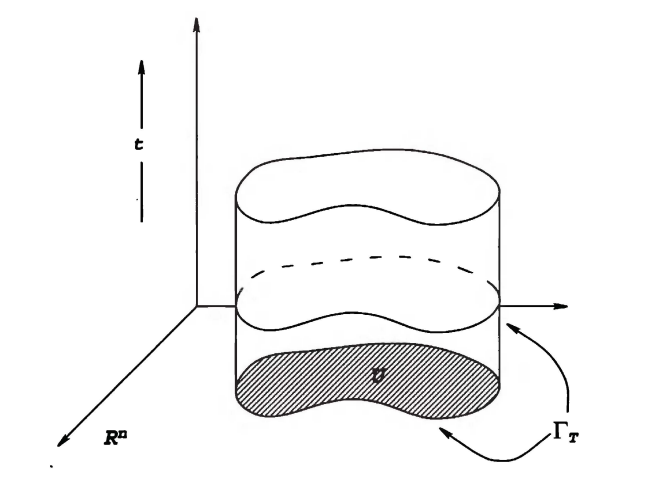
\includegraphics[scale=0.49]{Image/Parabolic Cylinder.png}
    \caption{The region $U_T$}
\end{figure}
We want next to derive a kind of analogue to the mean-value property as in the discussion of the Harmonic functions. There is no such simple formula. However let us observe that for fixed $x$ the spheres $\partial B(x,r)$ are level sets\footnote{A \textbf{level set} of a real-valued function is the set where the function take constant values, i.e. $L_c(f)=\{x\in\mathbb{R}^n:f(x)= c\}$.} of the fundamental solution $\Phi(x-y)$ for Laplace's function. This suggests that perhaps for fixed $(x,t)$ the level sets of fundamental solution $\Phi(x-y,t-s)$ for the heat equation may be relevant.
\begin{definition}
For fixed $x\in\mathbb{R}^n$, $t\in\mathbb{R}$ and $r>0$, we define a \textbf{heat ball}
$$
E\left( x,t;r \right) =\left\{ \left( y,s \right) \in \mathbb{R} ^{n+1}:s\le t,\Phi \left( x-y,t-s \right) \ge \frac{1}{r^n} \right\} .
$$
\end{definition}
\begin{figure}[htbp]
    \center
    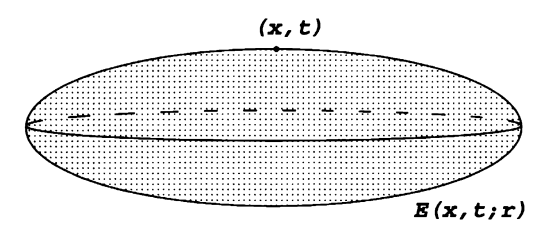
\includegraphics[scale=0.49]{Image/Heat Ball.png}
    \caption{A Heat Ball}
\end{figure}
This is a region in space-time, the boundary of which is a level set of $\Phi(x-y,t-s)$. Note that the point $(x,t)$ is at the center of the top.\par
We now introduce a mean-value property for the heat equations.
\begin{theorem}
Let $u\in C_1^2(U_T)$ solve the heat equation. Then 
$$
u\left( x,t \right) =\frac{1}{4r^n}\iint_{E\left( x,t;r \right)}{u\left( y,s \right) \frac{\left| x-y \right|^2}{\left( t-s \right) ^2}\mathrm{d}y\mathrm{d}s}
$$
for each $E(x,t;r)\subset U_T$.
\end{theorem}
\begin{proof}
Shift the space and time coordinates such that $x=0$ and $t=0$. We shall assume functions here are smooth, upon modifying if necessary. Write $E(0,0;r)=E(r)$. We define 
$$
\begin{aligned}
\phi \left( r \right) &=\frac{1}{r^n}\iint_{E\left( r \right)}{u\left( y,s \right) \frac{\left| y \right|^2}{s^2}\mathrm{d}y\mathrm{d}s}=\frac{1}{r^n}\iint_{E\left( 1 \right)}{u\left( ry,r^2s \right) \frac{\left| y \right|^2}{r^2s^2}\mathrm{d}ry\mathrm{d}r^2s}
\\
&=\frac{1}{r^{n+2}}\iint_{E\left( 1 \right)}{u\left( ry,r^2s \right) \frac{\left| y \right|^2}{s^2}r^n\mathrm{d}yr^2\mathrm{d}s}=\iint_{E\left( 1 \right)}{u\left( ry,r^2s \right) \frac{\left| y \right|^2}{s^2}\mathrm{d}y\mathrm{d}s}.
\end{aligned}
$$
Computing the derivative of $\phi$, we obtain 
$$
\begin{aligned}
\phi ^{\prime}\left( r \right) &=\iint_{E\left( 1 \right)}{\sum_{i=1}^n{y_i\cdot u_{y_i}\left( ry,r^2s \right) \frac{\left| y \right|^2}{s^2}}+2ru_s\left( ry,r^2s \right) \frac{\left| y \right|^2}{s}\mathrm{d}y\mathrm{d}s}
\\
&=\iint_{E\left( r \right)}{\sum_{i=1}^n{y_i\cdot u_{y_i}\left( y,s \right) \frac{r^2\left| y \right|^2}{s^2}+2ru_s\left( y,s \right) \frac{\left| y \right|^2}{s}\mathrm{d}\frac{y}{r}\mathrm{d}\frac{s}{r^2}}}
\\
&=\frac{1}{r^{n+1}}\iint_{E\left( r \right)}{\sum_{i=1}^n{y_i\cdot u_{y_i}\left( y,s \right) \frac{\left| y \right|^2}{s^2}}+2u_s\left( y,s \right) \frac{\left| y \right|^2}{s}\mathrm{d}y\mathrm{d}s}
\\
&=\mathop {\underbrace{\frac{1}{r^{n+1}}\iint_{E\left( r \right)}{\sum_{i=1}^n{y_i\cdot u_{y_i}\left( y,s \right) \frac{\left| y \right|^2}{s^2}}\mathrm{d}y\mathrm{d}s}}} \limits_{A}+\mathop {\underbrace{\frac{1}{r^{n+1}}\iint_{E\left( r \right)}{2u_s\left( y,s \right) \frac{\left| y \right|^2}{s}\mathrm{d}y\mathrm{d}s}}} \limits_{B}.
\end{aligned}
$$
Let us introduce a useful function 
$$
\psi =-\frac{n}{2}\log \left( -4\pi s \right) +\frac{\left| y \right|^2}{4s}+n\log r
$$
and observe that on $\partial E(r)$ we have 
$$
\Phi \left( y,-s \right) =\frac{1}{\left( -1 \right) ^{n/2}\left( 4\pi s \right) ^{n/2}}\exp \left( \frac{\left| y \right|^2}{4s} \right) =\frac{1}{r^n},
$$
this gives 
$$
\frac{\left| y \right|^2}{4s}-\frac{n}{2}\log \left( -4\pi s \right) =-n\log r
$$
and hence $\psi=0$ on $\partial E(r)\setminus\{(0,0)\}$. Also note that 
$$
\sum_{i=1}^n{y_i\psi _{y_i}}=\sum_{i=1}^n{y_i\cdot \frac{y_i}{2s}}=\frac{\left| y \right|^2}{2s},
$$
hence now we may utilize $\psi$ to write 
$$
\begin{aligned}
B&=\frac{1}{r^{n+1}}\iint_{E\left( r \right)}{4u_s\sum_{i=1}^n{y_i\psi _{y_i}}\mathrm{d}y\mathrm{d}s}=\frac{1}{r^{n+1}}\int_{\Omega}{\sum_{i=1}^n{\prod_{i=1}^n{\int_{a_i}^{b_i}{4u_sy_i\psi _{y_i}\mathrm{d}y_i}}}\mathrm{d}s}
\\
&=\frac{1}{r^{n+1}}\int_{\Omega}{\sum_{i=1}^n{\prod_{i=1}^n{\int_{a_i}^{b_i}{4u_sy_i\mathrm{d}\psi}}}\mathrm{d}s}=\frac{1}{r^{n+1}}\int_{\Omega}{\sum_{i=1}^n{\prod_{i=1}^n{\left( 4u_sy_i\psi \mid_{a_i}^{b_i}-\int_{a_i}^{b_i}{4u_s\psi +4u_{sy_i}y_i\psi \mathrm{d}y_i} \right)}}\mathrm{d}s}
\\
&=-\frac{1}{r^{n+1}}\int_{\Omega}{\sum_{i=1}^n{\prod_{i=1}^n{\int_{a_i}^{b_i}{4u_s\psi +4u_{sy_i}y_i\psi \mathrm{d}y_i}}}\mathrm{d}s}=-\frac{1}{r^{n+1}}\iint_{E\left( r \right)}{\sum_{i=1}^n{4u_s\psi +4u_{sy_i}y_i\psi}\mathrm{d}y\mathrm{d}s}
\\
&=-\frac{1}{r^{n+1}}\iint_{E\left( r \right)}{4nu_s\psi +\sum_{i=1}^n{4u_{sy_i}y_i\psi}\mathrm{d}y\mathrm{d}s}=\frac{1}{r^{n+1}}\iint_{E\left( r \right)}{-4nu_s\psi \mathrm{d}y\mathrm{d}s}+\frac{1}{r^{n+1}}\iint_{E\left( r \right)}{-\sum_{i=1}^n{4u_{sy_i}y_i\psi}\mathrm{d}y\mathrm{d}s}
\\
&=\frac{1}{r^{n+1}}\iint_{E\left( r \right)}{-4nu_s\psi \mathrm{d}y\mathrm{d}s}+\frac{1}{r^{n+1}}\iint_{E\left( r \right)}{-\sum_{i=1}^n{4u_{y_i}y_i\psi _s}\mathrm{d}y\mathrm{d}s}
\\
&=\frac{1}{r^{n+1}}\iint_{E\left( r \right)}{-4nu_s\psi \mathrm{d}y\mathrm{d}s}+\frac{1}{r^{n+1}}\iint_{E\left( r \right)}{-\sum_{i=1}^n{4u_{y_i}y_i\left( -\frac{n}{2s}-\frac{\left| y \right|^2}{4s^2} \right)}\mathrm{d}y\mathrm{d}s}
\\
&=\frac{1}{r^{n+1}}\iint_{E\left( r \right)}{-4nu_s\psi -\frac{2n}{s}\sum_{i=1}^n{u_{y_i}y_i}\mathrm{d}y\mathrm{d}s}-A.
\end{aligned}
$$
Therefore 
$$
\begin{aligned}
\phi ^{\prime}\left( r \right) &=A+B=\frac{1}{r^{n+1}}\iint_{E\left( r \right)}{-4nu_s\psi -\frac{2n}{s}\sum_{i=1}^n{u_{y_i}y_i}\mathrm{d}y\mathrm{d}s}
\\
&=\frac{1}{r^{n+1}}\iint_{E\left( r \right)}{-4n\Delta u\cdot \psi -\frac{2n}{s}\sum_{i=1}^n{u_{y_i}y_i}\mathrm{d}y\mathrm{d}s}
\\
&=\frac{1}{r^{n+1}}\sum_{i=1}^n{\iint_{E\left( r \right)}{-4nu_{y_i}\psi _{y_i}-\frac{2n}{s}u_{y_i}y_i\mathrm{d}y\mathrm{d}s}}=0,
\end{aligned}
$$
and hence $\phi$ a constant. Therefore 
$$
\phi \left( r \right) =\lim_{t\rightarrow 0} \phi \left( t \right) =u\left( 0,0 \right) \left( \lim_{t\rightarrow 0} \frac{1}{t^n}\iint_{E\left( t \right)}{\frac{\left| y^2 \right|}{s^2}\mathrm{d}y\mathrm{d}s} \right) =4u\left( 0,0 \right) .
$$
Therefore 
$$
\frac{1}{r^n}\iint_{E\left( r \right)}{u\left( y,s \right) \frac{\left| y \right|^2}{s^2}\mathrm{d}y\mathrm{d}s}=4u\left( 0,0 \right) 
$$
and the proof is finished.
\end{proof}
Now we employ the mean-value property to give a quick proof of the strong maximum principle.
\begin{theorem}\label{Thm1.3.6}
Assume $u\in C_1^2(U_T)\cap C(\overline{U_T})$ solves the heat equation in $U_T$.\par
(i) Then 
$$
\max_{\overline{U_T}} u=\max_{\Gamma _T} u.
$$\par
(ii) Furthermore, if $U$ is connected and there exists a point $(x_0,t_0)\in U_T$ such that 
$$
u\left( x_0,t_0 \right) =\max_{\overline{U_T}} u,
$$
then $u$ is a constant in $\overline{U_{t_0}}$.
\end{theorem}
\begin{figure}[htbp]
    \center
    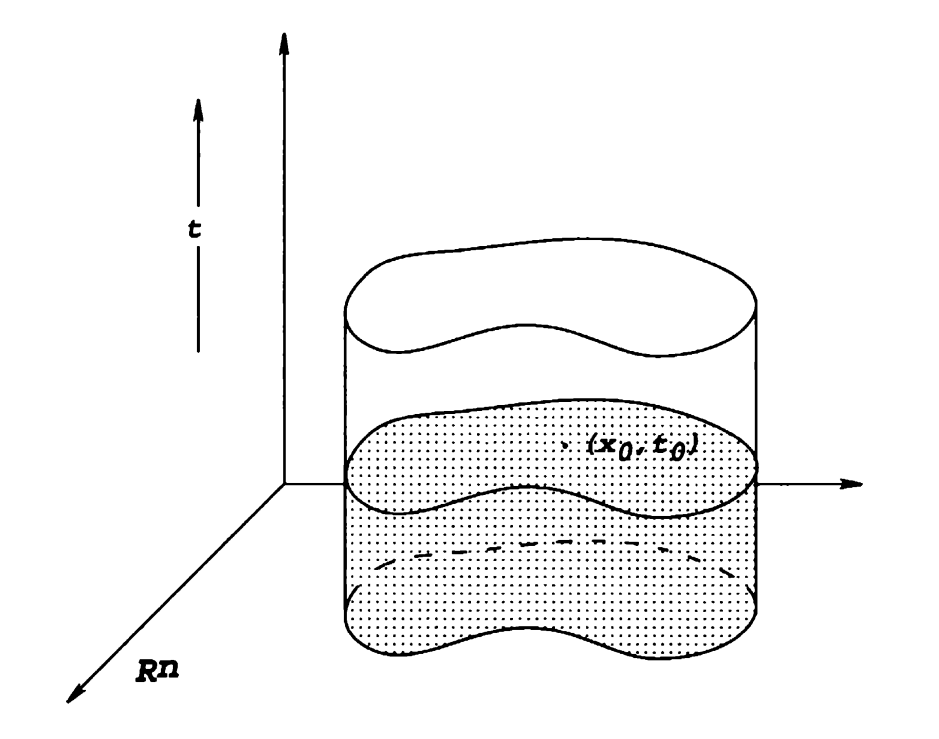
\includegraphics[scale=0.24]{Image/Strong Maximum Principle.png}
    \caption{The Strong Maximal Principle for Heat Equations}
\end{figure}
Assertion (i) is the \textbf{maximal principle} for the heat equation and assertion (ii) is the \textbf{strong maximal principle} for the heat equation.\par
The strong maximal principle accords with our strong intuitive understanding of the variable $t$ as denoting time: the solution will not change on the time interval $[0,t_0]$ provided the initial and boundary conditions are constant. However, the solution may change at times $t>t_0$, provided the boundary conditions alter after $t_0$. The solution will however not respond to changes in boundary conditions until those change happen.\par
We now give a proof of Theorem \ref{Thm1.3.6}.
\begin{proof}
We first proof (ii). Suppose $(x_0,t_0)\in U_T$ such that 
$$
u\left( x_0,t_0 \right) =M=\max_{\overline{U_T}} u.
$$
Then there exists some small $r$ such that the heat ball $E(x_0,r_0;r)\subset U_T$. Now we apply the mean-value property: 
$$
u\left( x_0,t_0 \right) =\frac{1}{4r^2}\iint_{E\left( x_0,r_0;r \right)}{u\left( x,t \right) \frac{\left| x_0-y \right|^2}{\left( t_0-s \right) ^2}\mathrm{d}y\mathrm{d}s}\le M\frac{1}{4r^2}\iint_{E\left( x_0,r_0;r \right)}{\frac{\left| x_0-y \right|^2}{\left( t_0-s \right) ^2}\mathrm{d}y\mathrm{d}s}=M.
$$
Note that the equality holds if and only if $u(x,t)\equiv M$ in $E(x_0,r_0,r)$.\par
Now suppose $(y_0,s_0)\in U_T$ such that $s_0<t_0$. Draw a line segment $L$ connecting $(x_0,t_0)$ and $(y_0,s_0)$. Consider 
$$
r_0=\min \left\{ s\ge s_0:u\left( x,t \right) =M \ \text{for all points $(x,t)\in L$},\ s\le t\le t_0\right\}. 
$$
We claim that $r_0=s_0$. If $r_0>s_0$, then $u(z_0,r_0)=M$ for some $z_0\in U$. Therefore by the mean-value property there exists a heat ball $E(z_0,r_0,r^\prime)\subset U_T$ contains $L\cap(r_0-\sigma,r_0)$, which contradict with the minimality of $r_0$. Therefore $s_0=r_0$ and hence $u(x,t)\equiv M$ for all $(x,t)\in L$.\par
Now for an arbitrary $x\in U$ and a time $t$, we may select $x_0,x_1,\cdots,x_m$ so that $x_i\in U$, $x_m=x$. Since $U$ is connected, there exists line segments that connect $x_{i-1}$ and $x_i$. Select time $t_0,t_1,\cdots,t_m$ so that $t_m=t$, $t_{i-1}>t_i$. Then the line segments in $\mathbb{R}^{n+1}$ connecting $(x_{i-1},t_{i-1})$ and $(x_i,t_i)$ lie in $U_T$. Therefore $u(x,t)=u(x_0,t_0)=M$. Since $(x,t)$ is arbitrarily chosen, we finished the proof.\par
Now we show that (i) follows from (ii). Suppose there exists some $(x_0,t_0)\in U_T$ that attained the maximum, then $u$ is a constant in $\overline{U_{t_0}}$, which extends to the boundary. Hence 
$$
\max_{\overline{U_T}} u=\max_{\Gamma _T} u
$$
and (i) follows from (ii).
\end{proof}
The strong maximum principle implies that if $U$ is connected and $u\in C_1^2(U_T)\cap C(\overline{U_T})$ satisfies 
\begin{equation}\label{1.35}
\left\{ \begin{aligned}
	u_t-\Delta u&=0\ \text{in}\ U_T\\
	u&=0\ \text{on}\ \partial U\times[0,T]\\
	u&=g\ \text{on}\ U\times\{t=0\}\\
\end{aligned} \right. 
\end{equation}
where $g\ge 0$, then $u$ is positive everywhere within $U_T$ if $g$ is positive somewhere on $U$. This is another illustration of infinite propagation speed for disturbances.\par
An important application of maximum principle is the following uniqueness assertion.
\begin{proposition}
Let $g\in C(U_T)$, $f\in C(U_T)$. Then there exists at most one solution $u\in C_1^2(U_T)\cap C(\overline{U_T})$ of the initial (boundary)-value problem 
\begin{equation}\label{1.99}
\left\{ \begin{aligned}
	u_t-\Delta u&=f\ \text{in}\ U_T\\
	u&=g\ \text{on}\ \Gamma_T.\\
\end{aligned} \right. 
\end{equation}
\end{proposition}
\begin{proof}
Suppose both $u$ and $\widetilde{u}$ are solutions of \eqref{1.35}. Then both $\pm(u-\widetilde{u})$ are solutions of \eqref{1.35} with $g=0$. Therefore by the maximum principle we have $u=\widetilde{u}=0$.
\end{proof}
We next extend our uniqueness assertion to the \textbf{Cauchy's problem}, that is, the initial-value problem for $U=\mathbb{R}^n$. As we no longer on a bounded region, we must introduce some control on the behavior of solutions for large $|x|$. We first proof the \textbf{maximum principle for the Cauchy problem}:
\begin{theorem}\label{Thm1.3.8}
Suppose $u\in C_1^2(\mathbb{R}^n\times(0,T])\cap C(\mathbb{R}^n\times[0,T])$ solves 
$$
\left\{ \begin{aligned}
	u_t-\Delta u&=0\ \text{in}\ \mathbb{R}^n\times(0,T)\\
	u&=g\ \text{on}\ \mathbb{R}^n\times\{t=0\}\
\end{aligned} \right. 
$$
and satisfies the growth estimate 
$$
u\left( x,t \right) \le Ae^{a\left| x \right|^2},\hspace{0.5cm}\left( x\in \mathbb{R} ^n,0\le t\le T \right) 
$$
for constants $A,a>0$. Then 
$$
\mathop {\mathrm{sup}} \limits_{\mathbb{R} ^n\times \left[ 0,T \right]}u=\mathop {\mathrm{sup}} \limits_{\mathbb{R} ^n}g.
$$
\end{theorem}
\begin{proof}
We may assume $4aT<1$, or otherwise consider $[0,T_1]$, $[T_1,T_2]$, $\cdots$ separately with $T_1=1/8a$. There exists some $\varepsilon>0$ such that $4a(T+\varepsilon)<1$. Fix $y\in\mathbb{R}^n$, $\nu>0$, and define 
$$
v\left( x,t \right) =u\left( x,t \right) -\frac{\mu}{\left( T+\varepsilon -t \right) ^{n/2}}\cdot \exp \left( \frac{\left| x-y \right|^2}{4\left( T+\varepsilon -t \right)} \right) ,\hspace{0.5cm}\left( x\in \mathbb{R} ^n,t>0 \right) 
$$
note that $v_t-\Delta v=0$ in $\mathbb{R}^n\times(0,T]$ by a direct calculation. Now fix $r>0$ and set $U=B(y,r)$ and $U_T=U\times(0,T]$. Then according to Theorem \ref{Thm1.3.6} we have 
$$
\max_{\overline{U_T}} v=\max_{\Gamma _T} v.
$$
Now if $x\in\mathbb{R}^n$, we have the estimates 
$$
v\left( x,0 \right) =u\left( x,0 \right) -\frac{\mu}{\left( T+\varepsilon \right) ^{n/2}}\cdot \exp \left( \frac{\left| x-y \right|^2}{4\left( T+\varepsilon \right)} \right) \le u\left( x,0 \right) =g\left( x \right) .
$$
If $|x-y|=r$ and $0\le t\le T$, we have the estimates 
$$
\begin{aligned}
v\left( x,t \right) &=u\left( x,t \right) -\frac{\mu}{\left( T+\varepsilon -t \right) ^{n/2}}\cdot \exp \left( \frac{\left| x-y \right|^2}{4\left( T+\varepsilon -t \right)} \right) \le Ae^{a\left| x \right|^2}-\frac{\mu}{\left( T+\varepsilon -t \right) ^{n/2}}\cdot \exp \left( \frac{\left| x-y \right|^2}{4\left( T+\varepsilon -t \right)} \right) 
\\
&\le Ae^{a\left( \left| y \right|+r \right) ^2}-\frac{\mu}{\left( T+\varepsilon \right) ^{n/2}}\cdot \exp \left( \frac{\left| x-y \right|^2}{4\left( T+\varepsilon \right)} \right) =Ae^{a\left( \left| y \right|+r \right) ^2}-4^{\frac{n}{2}}\mu \left( a+\gamma \right) ^{\frac{n}{2}}\cdot \exp \left( \left( a+\gamma \right) \left| x-y \right|^2 \right) 
\\
&=Ae^{a\left( \left| y \right|+r \right) ^2}-4^{\frac{n}{2}}\mu \left( a+\gamma \right) ^{\frac{n}{2}}\cdot \exp \left( \left( a+\gamma \right) r^2 \right),
\end{aligned}
$$
where $\gamma$ is taken such that 
$$
\frac{1}{4\left( T+\varepsilon \right)}=a+\gamma .
$$
Therefore for $r$ sufficiently large, we have $v(x,t)\le 0\le\sup_{\mathbb{R}^n}g$. Therefore combining all the estimates above, we obtain $v(y,t)\le\sup_{\mathbb{R}^n}g$ for all $y\in\mathbb{R}^n$ and $0\le t\le T$. Let $\mu\to 0$ to deduce the final result.
\end{proof}
\begin{proposition}\label{Prop.1.3.9}
Let $g\in C(\mathbb{R}^n)$, $f\in C(\mathbb{R}^n\times[0,T])$. Then there exists at most one solution $u\in C_1^2(\mathbb{R}^n\times(0,T])\cap C(\mathbb{R}^n\times[0,T])$ of the initial-value problem 
\begin{equation}\label{1.36}
\left\{ \begin{aligned}
	u_t-\Delta u&=f\ \text{in}\ \mathbb{R}^n\times(0,T)\\
	u&=g\ \text{on}\ \mathbb{R}^n\times\{t=0\}\
\end{aligned} \right. 
\end{equation}
satisfying the growth estimate 
$$
u\left( x,t \right) \le Ae^{a\left| x \right|^2},\hspace{0.5cm}\left( x\in \mathbb{R} ^n,0\le t\le T \right) 
$$
for constants $A,a>0$.
\end{proposition}
\begin{proof}
Suppose both $u$ and $\widetilde{u}$ are solutions of \eqref{1.36}. Then apply Theorem \ref{Thm1.3.8} on $\pm(u-\widetilde{u})$ to obtain $u=\widetilde{u}$.
\end{proof}
What happens if we omit the growth estimate over $u(x,t)$? Indeed, there are infinitely many solutions of \ref{1.36} without the control of growth estimate, see \cite{bers1964partial}. Each of these solutions besides $u\equiv 0$ grows very rapidly as $|x|\to\infty$. There is a very interesting thing here: Although $u\equiv0$ is certainly the "physically-correct" solution, the initial-value problem indeed admits other "nonphysically-correct" solutions. Proposition \ref{Prop.1.3.9} provided a criterion which excludes the "wrong" solutions.\par
We now demonstrate that solutions of the heat equation are automatically smooth.
\begin{theorem}\label{Thm1.3.10}
Suppose $u\in C_1^2(U_T)$ solves the heat equation in $U_T$, then $u\in C^\infty(U_T)$.
\end{theorem}
\begin{proof}
We use 
$$
C\left( x,t;r \right) =\left\{ \left( y,s \right) :\left| x-y \right|\le r,t-r^2\le s\le t \right\} 
$$
to denote a closed circular cylinder of radius $r$, height $r^2$, and top center point $(x,t)$.\par
Fix $(x_0,t_0)\in U_T$. Choose small $r$ such that $C=C(x_0,r_0;r)\subset U_T$. Then define $C^\prime=C(x_0,t_0;3r/4)$ and $C^{\prime\prime}=C(x_0,t_0;r/2)$. Now choose a smooth cutoff function $\zeta=\zeta(x,t)$ such that $0\le\zeta\le 1$, $\zeta\equiv 1$ on $C^\prime$ and $\zeta\equiv 0$ near the parabolic boundary of $C$. Extend $\zeta\equiv 0$ in $(\mathbb{R}^n\times[0,t_0])\setminus C$.\par
\begin{figure}[htbp]
    \center
    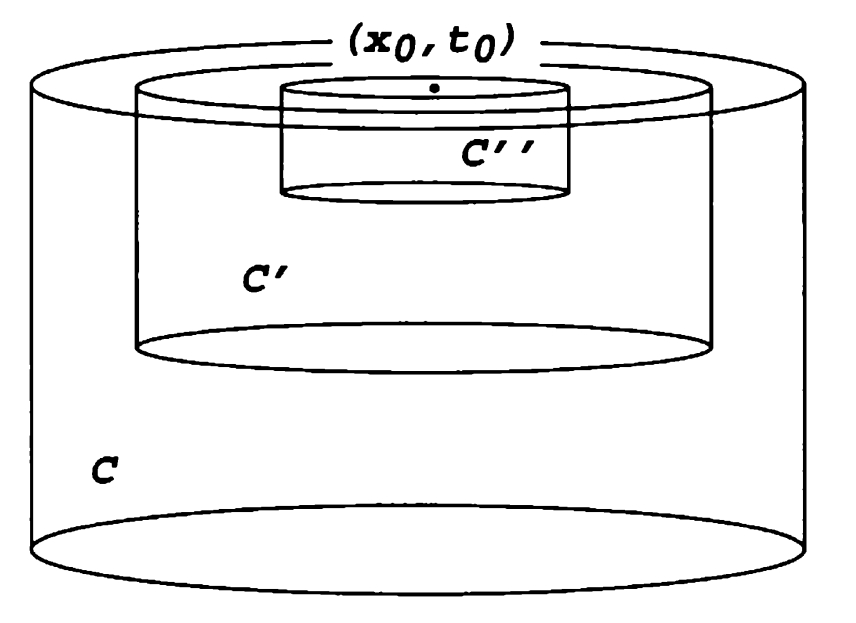
\includegraphics[scale=0.24]{Image/Circle Cylinders.png}
    \caption{The Set $C$, $C^\prime$ and $C^{\prime\prime}$}
\end{figure}
We shall first assume that $u\in C^\infty$. Note that this does not cause a circular argument, since we will eventually show that the final result obtained via this assumption does not actually rely on the smoothness of $u$, but only for a simplification of writing. We set $v(x,t)=\zeta(x,t)\cdot u(x,t)$ for $x\in\mathbb{R}^n$, $0\le t\le t_0$. Then 
$$
v_t=\zeta u_t+\zeta _tu,\hspace{0.5cm}\Delta u=\zeta \Delta u+2D\zeta \cdot Du+u\Delta \zeta .
$$
Consequently $v=0$ on $\mathbb{R}^n\times\{t=0\}$. If we set 
$$
\widetilde{f}\left( x,t \right) =\Delta u\left( x,t \right) =\zeta \left( x,t \right) \Delta u\left( x,t \right) +2D\zeta \left( x,t \right) \cdot Du\left( x,t \right) +u\left( x,t \right) \Delta \zeta \left( x,t \right) ,
$$
we obtain another solution 
$$
\widetilde{v}\left( x,t \right) =\int_0^t{\int_{\mathbb{R} ^n}{\Phi \left( x-y,s-t \right) \widetilde{f}\left( y,s \right) \mathrm{d}y}\mathrm{d}s}
$$
of the boundary-value problem \eqref{1.34} with $g=0$, since $|v|,|\widetilde{v}|\le A$ for some constant $A$. Then $v$ and $\widetilde{v}$ both are solutions to \eqref{1.34} with $g=0$, hence by Proposition \ref{Prop.1.3.9} we have $v=\widetilde{v}$; that is, 
$$
\widetilde{v}\left( x,t \right) =\int_0^t{\int_{\mathbb{R} ^n}{\Phi \left( x-y,s-t \right) \widetilde{f}\left( y,s \right) \mathrm{d}y}\mathrm{d}s}.
$$
Now suppose $(x,t)\in C^{\prime\prime}$. As $\zeta\equiv 0$ off the cylinder $C$, we have the following calculation: 
$$
\begin{aligned}
u\left( x,t \right) &=\int_0^t{\int_{\mathbb{R} ^n}{\Phi \left( x-y,t-s \right) \left[ \left( \zeta _s-\Delta \zeta \right) \left( y,s \right) u\left( y,s \right) -2D\zeta \left( y,s \right) \cdot Du\left( y,s \right) \right] \mathrm{d}y}\mathrm{d}s}
\\
&=\iint_C{\Phi \left( x-y,t-s \right) \left( \zeta _s-\Delta \zeta \right) \left( y,s \right) u\left( y,s \right) \mathrm{d}y\mathrm{d}s}-2\iint_C{\Phi \left( x-y,t-s \right) D\zeta \left( y,s \right) \cdot Du\left( y,s \right) \mathrm{d}y\mathrm{d}s}
\\
&=\iint_C{\Phi \left( x-y,t-s \right) \left( \zeta _s-\Delta \zeta \right) \left( y,s \right) u\left( y,s \right) \mathrm{d}y\mathrm{d}s}+2\iint_C{D_y\Phi \left( x-y,t-s \right) D\zeta \left( y,s \right) u\left( y,s \right) \mathrm{d}y\mathrm{d}s}
\\
&=\iint_C{\left[ \Phi \left( x-y,t-s \right) \left( \zeta _s-\Delta \zeta \right) \left( y,s \right) +2D_y\Phi \left( x-y,t-s \right) D\zeta \left( y,s \right) \right] \cdot u\left( y,s \right) \mathrm{d}y\mathrm{d}s}
\\
&=\iint_C{K\left( x,t,y,s \right) u\left( y,s \right) \mathrm{d}y\mathrm{d}s},
\end{aligned}
$$
where 
$$
K\left( x,t,y,s \right) =\Phi \left( x-y,t-s \right) \left( \zeta _s-\Delta \zeta \right) \left( y,s \right) +2D_y\Phi \left( x-y,t-s \right) D\zeta \left( y,s \right) .
$$
Now we assume that $u$ satisfies only the hypothesis of the theorem. Then apply the preceding discussion to $u^\varepsilon=\eta_\varepsilon*u$ instead of $u$ (see Appendices \ref{Appen.A}), we obtain 
$$
u^{\varepsilon}\left( x,t \right) =\iint_C{K\left( x,t,y,s \right) u^{\varepsilon}\left( y,s \right) \mathrm{d}y\mathrm{d}s}.
$$
Let $\varepsilon\to 0$, we still have 
\begin{equation}\label{1.37}
u\left( x,t \right) =\iint_C{K\left( x,t,y,s \right) u\left( y,s \right) \mathrm{d}y\mathrm{d}s}.
\end{equation}
Note that $K\equiv 0$ for all points $(y,s)\in C^\prime$ and smooth on $C\setminus C^\prime$. Therefore in the view of \eqref{1.37} we have $u\in C^\infty$ within $C^{\prime\prime}$. Since the choice of $(x_0,t_0)$ is arbitrary, we finished the proof.
\end{proof}
We now derive some estimates on the derivatives of solutions to the heat equation. Pay attention to the differences between derivatives with respect to $x_i$ and with respect to $t$.
\begin{theorem}
There exists for each pair of integers $k,l=0,1,\cdots$ a constant $C_{k,l}$ such that 
$$
\max_{C\left( x,t;r/2 \right)} \left| D_{x}^{k}D_{t}^{l}u \right|\le \frac{C_{kl}}{r^{k+2l+n+2}}\left\| u \right\| _{L^1\left( C\left( x,t;r \right) \right)}
$$
for all cylinders $C(x,t;r/2)\subset C(x,t;r)\subset U_T$ and all solutions $u$ of the heat equation in $U_T$.
\end{theorem}
\begin{proof}
Fix some point in $U_T$. We may assume by shifting the coordinates that the point is $(0,0)$. Suppose first that the cylinder $C(1)=C(0,0;1)$ lies in $U_T$. Let $C(1/2)=C(0,0;1/2)$. Then, as in the proof of Theorem \ref{Thm1.3.10}, we have 
$$
u\left( x,t \right) =\iint_{C\left( 1 \right)}{K\left( x,t,y,s \right) u\left( y,s \right) \mathrm{d}y\mathrm{d}s}
$$
for all $(x,t)\in C(1/2)$ and a smooth function $K$. Therefore 
$$
\left| D_{x}^{k}D_{t}^{l}u\left( x,t \right) \right|\le \iint_{C\left( 1 \right)}{\left| D_{x}^{k}D_{t}^{l}K\left( x,t,y,s \right) \right|\cdot \left| u\left( y,s \right) \right|\mathrm{d}y\mathrm{d}s}\le C_{kl}\left\| u \right\| _{L^1\left( C\left( 1 \right) \right)}
$$
for some constant $C_{kl}$.\par
Now assume the cylinder $C(r)=C(0,0;r)$ lies in $U_T$. Let $C(r/2)=C(0,0;r/2)$. We re-scale by defining $v(x,t)=u(rx,r^2t)$. Then $v_t-\Delta v=0$ is the cylinder $C(1)$ and hence 
$$
\left| D_{x}^{k}D_{t}^{l}v\left( x,t \right) \right|\le C_{kl}\left\| v \right\| _{L^1\left( C\left( 1 \right) \right)}
$$
for all $(x,t)\in C(1/2)$. However 
$$
\left| D_{x}^{k}D_{t}^{l}v\left( x,t \right) \right|=r^{2l+k}\left| D_{x}^{k}D_{t}^{l}u\left( rx,r^2t \right) \right|
$$
and 
$$
\left\| v \right\| _{L^1\left( C\left( 1 \right) \right)}=\frac{1}{r^{n+2}}\left\| u \right\| _{L^1\left( C\left( r \right) \right)},
$$
hence we have the estimate 
$$
\max_{C\left( r/2 \right)} \left| D_{x}^{k}D_{t}^{l}u \right|\le \frac{1}{r^{2l+k}}\max_{C\left( r/2 \right)} \left| D_{x}^{k}D_{t}^{l}v \right|\le \frac{C_{kl}}{r^{2l+k}}\left\| v \right\| _{L^1\left( C\left( 1 \right) \right)}=\frac{C_{kl}}{r^{k+2l+n+2}}\left\| u \right\| _{L^1\left( C\left( r \right) \right)},
$$
which finished the proof.
\end{proof}
\begin{note}\em
If $u$ solves the heat equation within $U_T$, then for each time $0\le t\le T$, the mapping $x\mapsto u(x,t)$ is analytic. However the mapping $t\mapsto u(x,t)$ is in general not analytic. See \cite{Mik1978partial}.
\end{note}
We investigate again the initial (boundary)-value problem \eqref{1.99}. We earlier invoked the maximum principle to show uniqueness and now, by an analogy with Theorem \ref{Thm1.2.24}, we provide an alternative argument based upon integration by parts. We assume as usual that $U\subset\mathbb{R}^n$ is open and bounded and that $\partial U$ is $C^1$. The terminal time $T>0$ is given.
\begin{theorem}
There exists only one solution $u\in C_1^2(\overline{U_T})$ of the initial (boundary)-value problem \eqref{1.99}.
\end{theorem}
\begin{proof}
If $\widetilde{u}$ is another solution, set $w=u-\widetilde{u}$, then $w$ solves \eqref{1.99} with $f=g=0$. Now set 
$$
e\left( t \right) =\int_U{w^2\left( x,t \right) \mathrm{d}x},\hspace{0.5cm}\left( 0\le t\le T \right) 
$$
then 
$$
\dot{e}\left( t \right) =2\int_U{ww_t\mathrm{d}x}=2\int_U{w\Delta w\mathrm{d}x}=-2\int_U{\left| Dw \right|^2\mathrm{d}x}\le 0,
$$
and so $e(t)\le e(0)=0$. Consequently $w=u-\widetilde{u}=0$ in $U_T$.
\end{proof}
A rather more subtle question asks about uniqueness \textit{backwards in time} for the heat equation. For this, suppose $u$ and $\widetilde{u}$ are both smooth solutions of the heat equation in $U_T$, with the same boundary conditions on $\partial U$ for some function $g$, i.e. we have 
\begin{equation}\label{1.38}
\left\{ \begin{aligned}
	u_t-\Delta u&=0\ \text{in}\ U_T\\
	u&=g\ \text{on}\ \partial U\times \left[ 0,T \right] ,\\
\end{aligned} \right. \hspace{0.5cm}\left\{ \begin{aligned}
	\widetilde{u}_t-\Delta \widetilde{u}&=0\ \text{in}\ U_T\\
	\widetilde{u}&=g\ \text{on}\ \partial U\times \left[ 0,T \right] ,\\
\end{aligned} \right. 
\end{equation}
Note that we are not supposing $u=\widetilde{u}$ at time $t=0$. Then we have the following 
\begin{theorem}
Suppose $u$ and $\widetilde{u}\in C_1^2(\overline{U_T})$ be in \eqref{1.38}. If $u(x,T)=\widetilde{u}(x,T)$, then $u\equiv\widetilde{u}$ within $U_T$.
\end{theorem}
In other words, if two temperature distributions on $U$ agree at some time $T>0$ and have had the same boundary values for times $0\le t\le T$, then these temperatures must have been identically equal within $U$ at all earlier times. This is not at all obvious.
\begin{proof}
Write $w=u-\widetilde{u}$. Define 
$$
e\left( t \right) =\int_U{w^2\left( x,t \right) \mathrm{d}x}\hspace{0.5cm}\left( 0\le t\le T \right) 
$$
as before, we have 
$$
\dot{e}\left( t \right) =-2\int_U{\left| Dw \right|^2\mathrm{d}x}\le 0
$$
and 
$$
\ddot{e}\left( t \right) =-4\int_U{Dw\cdot Dw_t\mathrm{d}x}=4\int_U{\Delta w\cdot w_t\mathrm{d}x}=4\int_U{\left( \Delta w \right) ^2\mathrm{d}x}.
$$
Now since $w=0$ on the boundary, we have 
$$
\int_U{\left| Dw \right|^2\mathrm{d}x}=-\int_U{w\Delta w\mathrm{d}x}\le \left( \int_U{w^2\mathrm{d}x} \right) ^{\frac{1}{2}}\cdot \left( \int_U{\Delta ^2w\mathrm{d}w} \right) ^{\frac{1}{2}}.
$$
Therefore 
$$
\left[ \dot{e}\left( t \right) \right] ^2=4\left( \int_U{\left| Dw \right|^2\mathrm{d}x} \right) ^2\le \left( \int_U{w^2\mathrm{d}x} \right) \cdot \left( \int_U{\Delta ^2w\mathrm{d}w} \right) =e\left( t \right) \ddot{e}\left( t \right) .
$$
Hence we obtain an ordinary differential equation 
$$
\left[ \dot{e}\left( t \right) \right] ^2\le e\left( t \right) \ddot{e}\left( t \right) .\hspace{0.5cm}\left( 0\le t\le T \right) 
$$\par
Now if $e(t)=0$ for all $t$, we are done. Otherwise there exists an interval $[t_1,t_2]\subset [0,T]$ such that $e(t)>0$ for $t_1\le t< t_2$ and $e(t_2)=0$. Write $f(t)=\log e(t)$, $t_1\le t<t_2$. Then we have 
$$
\ddot{f}\left( t \right) =\frac{\ddot{e}\left( t \right)}{e\left( t \right)}-\frac{\left[ \dot{e}\left( t \right) \right] ^2}{e^2\left( t \right)}=\frac{e\left( t \right) \ddot{e}\left( t \right) -\left[ \dot{e}\left( t \right) \right] ^2}{e^2\left( t \right)}\ge 0.
$$
So $f$ is convex on the interval $(t_1,t_2)$. Consequently if $0<\tau<1$ and $t_1<t<t_2$, we have 
$$
f\left( \left( 1-\tau \right) t_1+\tau t \right) \le \left( 1-\tau \right) f\left( t_1 \right) +\tau f\left( t \right) .
$$
This implies 
$$
e\left( \left( 1-\tau \right) t_1+\tau t \right) \le e^{1-\tau}\left( t_1 \right) e^{\tau}\left( t \right) ,
$$
and hence 
$$
0\le e\left( \left( 1-\tau \right) t_1+\tau t_2 \right) \le e^{1-\tau}\left( t_1 \right) e^{\tau}\left( t_2 \right) =0,
$$
a contradiction! Therefore $e(t)=0$ for all $t$ and hence $w=0$.
\end{proof}
\subsection{Wave Equation}
In this section we investigate the \textbf{wave equation}
\begin{equation}\label{1.40}
u_{tt}-\Delta u=0
\end{equation}
and the nonhomogeneous wave equation 
\begin{equation}\label{1.41}
u_{tt}-\Delta u=f,
\end{equation}
subject to appropriate initial and boundary conditions. Here $t>0$ and $x\in U$, where $U\subset\mathbb{R}^n$ is open. The unknown is $u:\overline{U}\times[0,\infty)\to\mathbb{R}$, $u=u(x,t)$, and the Laplacian $\Delta$ is taken with respect to the spatial variables $x=(x_1,\cdots,x_n)$. In \eqref{1.41} the function $f:U\times[0,\infty)\to\mathbb{R}$ is given. A common abbreviation is to write $\square u=u_{tt}-\Delta u$.\par
We shall discover the solutions of the wave equation behave quite differently than solutions of Laplace's equation or heat equation. For example, these solutions are generally not $C^\infty$, exhibit finite speed of propagation, etc.\par
We now find solutions to the wave equation. Instead of searching for certain scaling invariant solutions as Laplace's equation or heat equation, we will instead present an elegant method of solving \eqref{1.40} first for $n=1$ directly and then $n\ge 2$ by the method of spherical means.\par
We first focus on the following initial-value problem for one-dimensional wave equation in all of $\mathbb{R}$, i.e.  
\begin{equation}\label{1.42}
\left\{ \begin{aligned}
	u_{tt}-u_{xx}&=0\ \text{in}\ \mathbb{R}^n\times(0,\infty)\\
	u&=g\ \text{on}\ \mathbb{R}^n\times\{t=0\}\\
	u_t&=h\ \text{on}\ \mathbb{R}^n\times\{t=0\},\\
\end{aligned} \right. 
\end{equation}
where $n=1$, $g$ and $h$ are both given. We desire a formula for $u$ in terms of $g$ and $h$.\par
Let us first note that the PDE in \eqref{1.42} can be factored, to read 
$$
\left( \frac{\partial}{\partial t}+\frac{\partial}{\partial x} \right) \left( \frac{\partial}{\partial t}-\frac{\partial}{\partial x} \right) u=\frac{\partial ^2u}{\partial t^2}-\frac{\partial ^2u}{\partial x^2}=u_{tt}-u_{xx}=0.
$$
Write 
$$
v\left( x,t \right) =\left( \frac{\partial}{\partial t}-\frac{\partial}{\partial x} \right) u\left( x,t \right) .
$$
Then $v_t(x,t)+v_x(x,t)=0$ for $x\in\mathbb{R}$ and $t>0$. Therefore we have deduced the problem into a transport equation. Therefore apply \eqref{1.98}, we obtain 
$$
v\left( x,t \right) =v\left( x-t,0 \right) +\int_0^t{0\mathrm{d}s}=v\left( x-t,0 \right) .
$$
Now note the definition of $v$, we have 
$$
v\left( x,t \right) =u_t\left( x,t \right) -u_x\left( x,t \right) =v\left( x-t,0 \right) \ \text{in}\ \mathbb{R}^n\times(0,\infty).
$$
This is again a transport equation, hence we apply \eqref{1.98} again to obtain 
$$
u\left( x,t \right) =u\left( x+t,0 \right) +\int_0^t{v\left( x+\left( t-s \right) -s,0 \right) \mathrm{d}s}=u\left( x+t,0 \right) +\frac{1}{2}\int_{x-t}^{x+t}{v\left( y,0 \right) \mathrm{d}y}.
$$
By the initial condition we may determine $u(x,0)$ and $v(x,0)$. Therefore we may rewrite the solution as 
\begin{equation}\label{1.44}
u\left( x,t \right) =\frac{g\left( x+t \right) +g\left( x-t \right)}{2}+\frac{1}{2}\int_{x-t}^{x+t}{h\left( y \right) \mathrm{d}y}.\hspace{0.5cm}\left( x\in \mathbb{R} ,t\ge 0 \right) 
\end{equation}
This is \textbf{d'Alembert's formula}.\par
We have derived \eqref{1.44} by assuming $u$ sufficiently smooth. Now we need to check that this really is a solution.
\begin{theorem}
Assume $g\in C^2(\mathbb{R})$, $h\in C^1(\mathbb{R})$, and define $u$ by d'Alembert's formula \eqref{1.44}. Then \par
(i) $u\in C^2(\mathbb{R}\times[0,\infty))$;\par
(ii) $u_{tt}-u_{xx}=0$ in $\mathbb{R}\times(0,\infty)$;\par
(iii) $\lim_{(x,t)\to (x^0,0)}u(x,t)=g(x^0)$ and $\lim_{(x,t)\to (x^0,0)}u_t(x,t)=h(x^0)$ with $t>0$ for each $x^0\in\mathbb{R}$.
\end{theorem}
\begin{proof}
(i) Since $h\in C^1(\mathbb{R})$, the integral $\int_{x-t}^{x+t}{h\left( y \right) \mathrm{d}y}$ is in $C^2(\mathbb{R})$. Therefore $u$ is the sum of two $C^2$-components, hence $u\in C^2(\mathbb{R}\times[0,\infty))$.\par
(ii) This follows from a direct computation.\par
(iii) We only proof for the first limit. Note that $u(x,t)$ is $C^2$, we have 
$$
\lim_{(x,t)\rightarrow (x^0,0)} u(x,t)=u(x^0,0)=\frac{g(x^0)+g(x^0)}{2}+\frac{1}{2}\int_x^x{h\left( y \right) \mathrm{d}y}=g(x^0).
$$
The second limit may be proved in an analogous way.
\end{proof}
\begin{note}\em
(i) In view of \eqref{1.44}, our solution $u$ has the form $u(x,t)=F(x+t)+G(x-t)$ for appropriate functions $F$ and $G$. Conversely any function of this form solves $u_{tt}-u_{xx}=0$. Hence the general solution of the one-dimensional wave equation is a sum of the general solution $u_t-u_x=0$ and the general solution of $u_t+u_x=0$. This is a consequence of the factorization of $u_{tt}-u_{xx}=0$.\par
(ii) We see from \eqref{1.44} that if $g\in C^k$ and $h\in C^{k-1}$, then $u\in C^k$ but is not in general smoother. Thus the wave equation does not cause instantaneous smoothing of the initial data, as does the heat equation.
\end{note}
To illustrate a further application of d'Alembert's formula, let us consider this initial (boundary)-value problem on the half-plane $\mathbb{R}_+=\{x>0\}$: 
\begin{equation}\label{1.45}
\left\{ \begin{aligned}
	u_{tt}-u_{xx}&=0\ \text{in}\ \mathbb{R}_+\times(0,\infty)\\
	u=g,u_t&=h\ \text{on}\ \mathbb{R}_+\times\{t=0\}\\
	u&=0\ \text{on}\ \{x=0\}\times(0,\infty),\\
\end{aligned} \right. 
\end{equation}
where $g,h$ are given, with $g(0)=h(0)=0$. We convert \eqref{1.45} into the form \eqref{1.42} by reflecting $u$, $g$ and $h$ to all of $\mathbb{R}$ by odd reflection. That is, we set 
$$
\widetilde{u}\left( x,t \right) =\left\{ \begin{aligned}
	u\left( x,t \right) &\left( x\ge 0,t\ge 0 \right)\\
	-u\left( -x,t \right) &\left( x\le 0,t\ge 0 \right)\\
\end{aligned} \right. ,\hspace{0.5cm}\widetilde{g}\left( x \right) =\left\{ \begin{aligned}
	g\left( x \right) &\left( x\ge 0 \right)\\
	-g\left( -x \right) &\left( x\le 0 \right)\\
\end{aligned} \right. ,\hspace{0.5cm}\widetilde{h}\left( x \right) =\left\{ \begin{aligned}
	h\left( x \right) &\left( x\ge 0 \right)\\
	-h\left( -x \right) &\left( x\le 0 \right)\\
\end{aligned} \right. .
$$
Then \eqref{1.45} becomes 
$$
\left\{ \begin{aligned}
	\widetilde{u}_{tt}-\widetilde{u}_{xx}&=0\ \text{in}\ \mathbb{R}\times(0,\infty)\\
	\widetilde{u}=\widetilde{g},\widetilde{u}_t&=\widetilde{h}\ \text{on}\ \mathbb{R}\times\{t=0\}.\\
\end{aligned} \right. 
$$
Hence by d'Alembert's formula we have 
\begin{equation}\label{1.97}
\widetilde{u}\left( x,t \right) =\frac{\widetilde{g}\left( x+t \right) +\widetilde{g}\left( x-t \right)}{2}+\frac{1}{2}\int_{x-t}^{x+t}{\widetilde{h}\left( y \right) \mathrm{d}y}=\left\{ \begin{aligned}
	\frac{1}{2}\left[ g\left( x+t \right) +g\left( x-t \right) \right] +\frac{1}{2}\int_{x-t}^{x+t}{h\left( y \right) \mathrm{d}y}&x\ge t\ge 0\\
	\frac{1}{2}\left[ g\left( t+x \right) +g\left( t-x \right) \right] +\frac{1}{2}\int_{t-x}^{t+x}{h\left( y \right) \mathrm{d}y}&0\le x\le t.\\
\end{aligned} \right. 
\end{equation}
Note that our solution does not belong to $C^2$ in this case unless $g^{\prime\prime}(0)=0$.\par
Now suppose $n\ge 2$, $m\ge 2$, and $u\in C^m(\mathbb{R}^n\times[0,\infty))$ solves the initial-value problem \eqref{1.42}. We intend to derive a formula for $u$ in terms of $g,h$. The plan will be to study first the average of $u$ over certain spheres. These averages, taken as functions of the time $t$ and their radius $r$, turn out to solve the Euler-Poisson-Darboux equation, a PDE which can for odd $n$ convert into the ordinary one-dimensional wave equation. Applying d'Alembert's formula we eventually obtain a formula for the solution.\par
We first introduce some notations. Let $x\in\mathbb{R}^n$, $t>0$, $r>0$. We define 
\begin{equation}\label{1.96}
U\left( x;r,t \right) =\fint_{\partial B\left( x,r \right)}{u\left( y,t \right) \mathrm{d}S\left( y \right)},
\end{equation}
the average of $u(\cdot,t)$ over the sphere $\partial B(x,r)$. Similarly, we define the average of $g$ and $h$ to be 
$$
G\left( x;r \right) =\fint_{\partial B\left( x,r \right)}{g\left( y \right) \mathrm{d}S\left( y \right)},\hspace{0.5cm}H\left( x;r \right) =\fint_{\partial B\left( x,r \right)}{h\left( y \right) \mathrm{d}S\left( y \right)}.
$$
For fixed $x$, we hereafter regard $U$ as a function of $r$ and $t$ and discover a partial differential equation that $U$ solves: 
\begin{lemma}\em
Fix $x\in\mathbb{R}^n$, and let $u$ satisfy \eqref{1.42}. Then $U\in C^m(\overline{\mathbb{R}_+}\times[0,\infty))$ and 
\begin{equation}
\left\{ \begin{aligned}\label{1.46}
	U_{tt}-U_{rr}-\frac{n-1}{r}U_r&=0\ \text{in}\ \mathbb{R}_+\times(0,\infty)\\
	U=G,U_t&=H\ \text{on}\ \mathbb{R}_+\times\{t=0\}\\
\end{aligned} \right. 
\end{equation}
\end{lemma}
The partial differential equation \eqref{1.46} is called the \textbf{Euler-Poisson-Darboux equation}. Note that $U_{rr}+\frac{n-1}{r}U_r$ is the radial part of the Laplacian $\Delta$ in polar coordinates.
\begin{proof}
We first notice that 
$$
U\left( x;r,t \right) =\fint_{\partial B\left( x,r \right)}{u\left( y,t \right) \mathrm{d}S\left( y \right)}=\fint_{\partial \left( 0,1 \right)}{u\left( x+rz,t \right) \mathrm{d}S\left( z \right)}.
$$
Therefore 
$$
\begin{aligned}
U_r\left( x;r,t \right) &=\fint_{\partial B\left( 0,1 \right)}{z\cdot u_x\left( x+rz,t \right) \mathrm{d}S\left( z \right)}=\fint_{\partial B\left( x,r \right)}{\frac{y-x}{r}\cdot u_x\left( y,t \right) \mathrm{d}S\left( y \right)}
\\
&=\fint_{\partial B\left( x,r \right)}{\frac{\partial u}{\partial \nu}\left( y,t \right) \mathrm{d}S\left( y \right)}=\frac{r}{n}\fint_{B\left( x,r \right)}{\Delta u\left( y,t \right) \mathrm{d}y}.
\end{aligned}
$$
Hence we have $U_r(x;r,t)\to 0$ as $r\to 0$. We further differentiate $U_r$. First note that 
$$
r^{n-1}U_r\left( x;r,t \right) =\frac{1}{n\alpha \left( n \right)}\int_{B\left( x,r \right)}{\Delta u\left( y,t \right) \mathrm{d}y},
$$
differentiate on both side to obtain 
$$
r^{n-1}U_{rr}\left( x;r,t \right) +\left( n-1 \right) r^{n-2}U_r\left( x;r,t \right) =\frac{1}{n\alpha \left( n \right)}\int_{\partial B\left( x,r \right)}{\Delta u\left( y,t \right) \mathrm{d}S\left( y \right)},
$$
where the right-hand-side follows from the following calculation: 
$$
\begin{aligned}
\frac{\partial}{\partial r}\int_{B\left( x,r \right)}{\Delta u\left( y,t \right) \mathrm{d}y}&=\frac{\partial}{\partial r}\int_{B\left( 0,1 \right)}{\Delta u\left( x+rz,t \right) \mathrm{d}z}=\int_{B\left( 0,1 \right)}{z\cdot D_x\Delta u\left( x+rz,t \right) \mathrm{d}z}
\\
&=\int_{B\left( x,r \right)}{\frac{y-x}{r}\cdot D_x\Delta u\left( y,t \right) \mathrm{d}y}=\int_{B\left( x,r \right)}{\frac{\partial \Delta u}{\partial \nu}\left( y,t \right) \mathrm{d}y}=\int_{\partial B\left( x,r \right)}{\Delta u\left( y,t \right) \mathrm{d}S\left( y \right)}.
\end{aligned}
$$
Now we have 
$$
\begin{aligned}
U_{rr}\left( x;r,t \right) &=\frac{1}{n\alpha \left( n \right)}\int_{\partial B\left( x,r \right)}{\Delta u\left( y,t \right) \mathrm{d}S\left( y \right)}-\frac{n-1}{r}U_r\left( x;r,t \right) 
\\
&=\frac{1}{n\alpha \left( n \right)}\int_{\partial B\left( x,r \right)}{\Delta u\left( y,t \right) \mathrm{d}S\left( y \right)}-\frac{n-1}{r}\cdot \frac{r}{n}\fint_{B\left( x,r \right)}{\Delta u\left( y,t \right) \mathrm{d}y}
\\
&=\fint_{\partial B\left( x,r \right)}{\Delta u\mathrm{d}S}-\frac{n-1}{n}\fint_{B\left( x,r \right)}{\Delta u\mathrm{d}y}.
\end{aligned}
$$
Therefore $U_{rr}\to \Delta u(x,t)/n$ as $r\to 0$. If we continue to calculate $U_{rrr}$ we obtain the similar result. Therefore $U\in C^m(\overline{\mathbb{R}_+}\times[0,\infty))$.\par
Now we prove that $U$ solve the equation \eqref{1.46}. Indeed, note that 
$$
U_r=\frac{r}{n}\fint_{B\left( x,r \right)}{\Delta u\mathrm{d}y}=\frac{r}{n}\fint_{B\left( x,r \right)}{u_{tt}\mathrm{d}y}=\frac{1}{nr^{n-1}\alpha \left( n \right)}\int_{B\left( x,r \right)}{u_{tt}\mathrm{d}y},
$$
we have 
$$
r^{n-1}U_r=\frac{1}{n\alpha \left( n \right)}\int_{B\left( x,r \right)}{u_{tt}\mathrm{d}y}.
$$
Differentiate with respect to $r$ on both hands we have 
$$
r^{n-1}U_{rr}+\left( n-1 \right) r^{n-2}U_r=\frac{1}{n\alpha \left( n \right)}\int_{\partial B\left( x,r \right)}{u_{tt}\mathrm{d}S}=r^{n-1}\fint_{\partial B\left( x,r \right)}{u_{tt}\mathrm{d}S}=r^{n-1}U_{tt},
$$
which finished the proof.
\end{proof}
The plan in the ensuing subsections will be to transform the Euler-Poisson-Darboux equation into the usual one-dimensional wave equation. As the full procedure is rather complicated, we pause here to handle the simpler cases $n=3,2$, in that order.\par
Let us hereafter take $n=3$, and suppose $u\in C^2(\mathbb{R}^n\times[0,\infty))$ solves the initial-value problem \eqref{1.42}. If we set 
$$
\widetilde{U}=rU,\hspace{0.5cm}\widetilde{G}=rG,\hspace{0.5cm}\widetilde{H}=rH,
$$
we assert that $\widetilde{U}$ solves the equation 
\begin{equation}\label{1.48}
\left\{ \begin{aligned}
	\widetilde{U_{tt}}-\widetilde{U_{rr}}&=0\ \text{in}\ \mathbb{R}_+\times(0,\infty)\\
	\widetilde{U}=\widetilde{G},\widetilde{U_t}&=\widetilde{H}\ \text{on}\ \mathbb{R}_+\times\{t=0\}\\
	\widetilde{U}&=0\ \{r=0\}\times(0,\infty)\\
\end{aligned} \right. 
\end{equation}
Indeed we have 
$$
\widetilde{U_{tt}}=rU_{tt}=r\left( U_{rr}+\frac{n-1}{r}U_r \right) =rU_{rr}+\left( n-1 \right) rU_r=\frac{\partial}{\partial r}\left( U+rU_r \right) =\widetilde{U_{rr}},
$$
and the second and the third equation holds trivially. Therefore 
\begin{equation}\label{1.95}
\begin{aligned}
u\left( x,r \right) &=\lim_{r\rightarrow 0^+} U\left( x;r,t \right) =\lim_{r\rightarrow 0^+} \frac{\widetilde{U}\left( x;r,t \right)}{r}
\\
&=\lim_{r\rightarrow 0^+} \left[ \frac{\widetilde{G}\left( t+r \right) -\widetilde{G}\left( t-r \right)}{2r}+\frac{1}{2r}\int_{-r+t}^{r+t}{\widetilde{H}\left( y \right) \mathrm{d}y} \right] =\widetilde{G}^{\prime}\left( t \right) +\widetilde{H}\left( t \right) 
\\
&=\frac{\partial}{\partial t}\left( t\fint_{\partial B\left( x,t \right)}{g\left( y \right) \mathrm{d}S\left( y \right)} \right) +t\fint_{\partial B\left( x,t \right)}{h\left( y \right) \mathrm{d}S\left( y \right)}
\\
&=\fint_{\partial B\left( x,t \right)}{g\left( y \right) \mathrm{d}S\left( y \right)}+t\cdot \frac{\partial}{\partial t}\left( \fint_{\partial B\left( x,t \right)}{g\left( y \right) \mathrm{d}S\left( y \right)} \right) +t\fint_{\partial B\left( x,t \right)}{h\left( y \right) \mathrm{d}S\left( y \right)}
\\
&=\fint_{\partial B\left( x,t \right)}{g\left( y \right) \mathrm{d}S\left( y \right)}+t\cdot \frac{\partial}{\partial t}\left( \fint_{\partial B\left( 0,1 \right)}{g\left( x+tz \right) \mathrm{d}S\left( z \right)} \right) +t\fint_{\partial B\left( x,t \right)}{h\left( y \right) \mathrm{d}S\left( y \right)}
\\
&=\fint_{\partial B\left( x,t \right)}{g\left( y \right) \mathrm{d}S\left( y \right)}+t\cdot \fint_{\partial B\left( 0,1 \right)}{z\cdot Dg\left( x+tz \right) \mathrm{d}S\left( z \right)}+t\fint_{\partial B\left( x,t \right)}{h\left( y \right) \mathrm{d}S\left( y \right)}
\\
&=\fint_{\partial B\left( x,t \right)}{g\left( y \right) \mathrm{d}S\left( y \right)}+t\cdot \fint_{\partial B\left( x,t \right)}{\frac{y-x}{t}\cdot Dg\left( y \right) \mathrm{d}S\left( y \right)}+t\fint_{\partial B\left( x,t \right)}{h\left( y \right) \mathrm{d}S\left( y \right)}
\\
&=\fint_{\partial B\left( x,t \right)}{t\cdot h\left( y \right) +g\left( y \right) +Dg\left( y \right) \cdot \left( y-x \right) \mathrm{d}S\left( y \right)}.
\end{aligned}
\end{equation}
This gives us the following \textbf{Kirchhoff's formula} 
$$
u\left( x,r \right) =\fint_{\partial B\left( x,t \right)}{t\cdot h\left( y \right) +g\left( y \right) +Dg\left( y \right) \cdot \left( y-x \right) \mathrm{d}S\left( y \right)}
$$
for the solution of the initial-value problem \eqref{1.42} in three dimensions.\par
Now we solve \eqref{1.42} with $n=2$. Unfortunately, no transformations as $\widetilde{U}=rU$ works here. Instead, we shall adopt the \textbf{method of descent} here: regarding the initial-value problem \eqref{1.42} as a three-dimensional problem, in which the third variable $x_3$ does not appear.\par
Assume $u\in C^2(\mathbb{R}^2\times[0,\infty))$ solves \eqref{1.42} when $n=2$, let us write $\overline{u}(x_1,x_2,x_3,t)=u(x_1,x_2,t)$. Then we have 
$$
\left\{ \begin{aligned}
	\overline{u_{tt}}-\Delta \overline{u}&=0\ \text{in}\ \mathbb{R}^3\times(0,\infty)\\
	\overline{u}=\overline{g},\overline{u_t}&=\overline{h}\ \text{on}\ \mathbb{R}^3\times\{t=0\},\\
\end{aligned} \right. 
$$
for 
$$
\overline{g}\left( x_1,x_2,x_3 \right) =g\left( x_1,x_2 \right) ;\hspace{0.5cm}\overline{h}\left( x_1,x_2,x_3 \right) =h\left( x_1,x_2 \right) .
$$
If we write $x=(x_1,x_2)\in\mathbb{R}^2$ and $\overline{x}=(x_1,x_2,0)\in\mathbb{R}^3$, then by Kirchhoff's formula we have 
$$
u\left( x,t \right) =\overline{u}\left( \overline{x},t \right) =\frac{\partial}{\partial t}\left( t\fint_{\partial \overline{B}\left( \overline{x},t \right)}{\overline{g}\mathrm{d}\overline{S}} \right) +t\fint_{\partial \overline{B}\left( \overline{x},t \right)}{\overline{h}\mathrm{d}\overline{S}},
$$
where $\overline{B}(\overline{x},t)$ denote the ball in $\mathbb{R}^3$ with center $\overline{x}$, radius $t>0$ and $\mathrm{d}\overline{S}$ denote the two-dimensional surface measure on $\partial\overline{B}(\overline{x},t)$. Define $\gamma(t)=(t^2-|y-x|^2)^{1/2}$ for $y\in B(x,t)$. Therefore we may simplify as follows: 
$$
\begin{aligned}
u\left( x,t \right) &=\frac{\partial}{\partial t}\left( t\fint_{\partial \overline{B}\left( \overline{x},t \right)}{\overline{g}\mathrm{d}\overline{S}} \right) +t\fint_{\partial \overline{B}\left( \overline{x},t \right)}{\overline{h}\mathrm{d}\overline{S}}
\\
&=\frac{\partial}{\partial t}\left( \frac{1}{4\pi t}\int_{\partial \overline{B}\left( \overline{x},t \right)}{\overline{g}\mathrm{d}\overline{S}} \right) +t\fint_{\partial \overline{B}\left( \overline{x},t \right)}{\overline{h}\mathrm{d}\overline{S}}
\\
&=\frac{\partial}{\partial t}\left( \frac{1}{2\pi t}\int_{B\left( x,t \right)}{g\left( y \right) \cdot \left( 1+\left| D\gamma \left( y \right) ^2 \right| \right) ^{\frac{1}{2}}\mathrm{d}y} \right) +\frac{1}{2\pi t}\int_{B\left( x,t \right)}{h\left( y \right) \cdot \left( 1+\left| D\gamma \left( y \right) ^2 \right| \right) ^{\frac{1}{2}}\mathrm{d}y}
\\
&=\frac{\partial}{\partial t}\left( \frac{1}{2\pi}\int_{B\left( x,t \right)}{\frac{g\left( y \right)}{\left( t^2-\left| y-x \right|^2 \right) ^{\frac{1}{2}}}\mathrm{d}y} \right) +\frac{1}{2\pi}\int_{B\left( x,t \right)}{\frac{h\left( y \right)}{\left( t^2-\left| y-x \right|^2 \right) ^{\frac{1}{2}}}\mathrm{d}y}
\\
&=\frac{1}{2}\frac{\partial}{\partial t}\left( t^2\fint_{B\left( x,t \right)}{\frac{g\left( y \right)}{\left( t^2-\left| y-x \right|^2 \right) ^{\frac{1}{2}}}\mathrm{d}y} \right) +\frac{t^2}{2}\fint_{B\left( x,t \right)}{\frac{h\left( y \right)}{\left( t^2-\left| y-x \right|^2 \right) ^{\frac{1}{2}}}\mathrm{d}y}
\\
&=\frac{1}{2}\frac{\partial}{\partial t}\left( t\fint_{B\left( 0,1 \right)}{\frac{g\left( x+tz \right)}{\left( 1-\left| z \right|^2 \right) ^{\frac{1}{2}}}\mathrm{d}z} \right) +\frac{t^2}{2}\fint_{B\left( x,t \right)}{\frac{h\left( y \right)}{\left( t^2-\left| y-x \right|^2 \right) ^{\frac{1}{2}}}\mathrm{d}y}
\\
&=\fint_{B\left( 0,1 \right)}{\frac{g\left( x+tz \right)}{\left( 1-\left| z \right|^2 \right) ^{\frac{1}{2}}}\mathrm{d}z}+t\fint_{B\left( 0,1 \right)}{\frac{z\cdot Dg\left( x+tz \right)}{\left( 1-\left| z \right|^2 \right) ^{\frac{1}{2}}}\mathrm{d}z}+\frac{t^2}{2}\fint_{B\left( x,t \right)}{\frac{h\left( y \right)}{\left( t^2-\left| y-x \right|^2 \right) ^{\frac{1}{2}}}\mathrm{d}y}
\\
&=t\fint_{B\left( x,t \right)}{\frac{g\left( y \right)}{\left( t^2-\left| y-x \right|^2 \right) ^{\frac{1}{2}}}\mathrm{d}y}+t\fint_{B\left( x,t \right)}{\frac{Dg\left( y \right) \cdot \left( y-x \right)}{\left( t^2-\left| y-x \right|^2 \right) ^{\frac{1}{2}}}\mathrm{d}y}+\frac{t^2}{2}\fint_{B\left( x,t \right)}{\frac{h\left( y \right)}{\left( t^2-\left| y-x \right|^2 \right) ^{\frac{1}{2}}}\mathrm{d}y}
\\
&=\frac{1}{2}\fint_{B\left( x,t \right)}{\frac{tg\left( y \right) +t^2h\left( y \right) +tDg\left( y \right) \cdot \left( y-x \right)}{\left( t^2-\left| y-x \right|^2 \right) ^{\frac{1}{2}}}\mathrm{d}y}.
\end{aligned}
$$
Therefore we obtain the \textbf{Poisson's formula} 
$$
u\left( x,t \right) =\frac{1}{2}\fint_{B\left( x,t \right)}{\frac{tg\left( y \right) +t^2h\left( y \right) +tDg\left( y \right) \cdot \left( y-x \right)}{\left( t^2-\left| y-x \right|^2 \right) ^{\frac{1}{2}}}\mathrm{d}y}
$$
for the solution of the initial-value problem \eqref{1.42} in two dimensions.\par
Now we solve the Euler-Poisson-Darboux PDE for odd $n\ge 3$. We first record some technical facts.
\begin{lemma}\em\label{Lem1.4.2}
Let $\phi:\mathbb{R}\to\mathbb{R}$ be $C^{k+1}$. Then for $k=1,2,\cdots$, we have \par
(i) The identity 
$$
\left( \frac{\mathrm{d}^2}{\mathrm{d}r^2} \right) \left( \frac{1}{r}\cdot \frac{\mathrm{d}}{\mathrm{d}r} \right) ^{k-1}\left( r^{2k-1}\phi \left( r \right) \right) =\left( \frac{1}{r}\cdot \frac{\mathrm{d}}{\mathrm{d}r} \right) ^k\left( r^{2k}\frac{\mathrm{d}\phi}{\mathrm{d}r}\left( r \right) \right) .
$$\par
(ii) There exists some constant $\beta_j^k$ that are independent of $\phi$ such that 
$$
\left( \frac{1}{r}\cdot \frac{\mathrm{d}}{\mathrm{d}r} \right) ^{k-1}\left( r^{2k-1}\phi \left( r \right) \right) =\sum_{j=0}^{k-1}{\beta _{j}^{k}r^{j+1}\frac{\mathrm{d}^j\phi}{\mathrm{d}r^j}\left( r \right)},
$$
and $\beta_0^k=(2k-1)!!$.
\end{lemma}
\begin{proof}
(i) We prove by induction. For $k=1$, we observe that the left hand side 
$$
\frac{\mathrm{d}^2}{\mathrm{d}r^2}\left( r\phi \left( r \right) \right) =\frac{\mathrm{d}}{\mathrm{d}r}\left( \phi \left( r \right) +r\phi ^{\prime}\left( r \right) \right) =\phi ^{\prime}\left( r \right) +\phi ^{\prime}\left( r \right) +r\phi ^{\prime\prime}\left( r \right) =2\phi ^{\prime}\left( r \right) +r\phi ^{\prime\prime}\left( r \right) ,
$$
while the right hand side 
$$
\left( \frac{1}{r}\cdot \frac{\mathrm{d}}{\mathrm{d}r} \right) \left( r^2\phi ^{\prime}\left( r \right) \right) =\frac{2r\phi ^{\prime}\left( r \right) +r^2\phi ^{\prime\prime}\left( r \right)}{r}=2\phi ^{\prime}\left( r \right) +r\phi ^{\prime\prime}\left( r \right) .
$$
Therefore the identity holds when $k=1$. Now we suppose this is true for all $k<n$, we now show the condition of $k=n$. By a direct calculation we obtain 
$$
\begin{aligned}
\left( \frac{\mathrm{d}^2}{\mathrm{d}r^2} \right) \left( \frac{1}{r}\cdot \frac{\mathrm{d}}{\mathrm{d}r} \right) ^{n-1}\left( r^{2n-1}\phi \left( r \right) \right) &=\left( \frac{\mathrm{d}^2}{\mathrm{d}r^2} \right) \left( \frac{1}{r}\cdot \frac{\mathrm{d}}{\mathrm{d}r} \right) ^{n-2}\left( \frac{1}{r}\cdot \frac{\mathrm{d}}{\mathrm{d}r} \right) \left( r^{2n-1}\phi \left( r \right) \right) 
\\
&=\left( \frac{\mathrm{d}^2}{\mathrm{d}r^2} \right) \left( \frac{1}{r}\cdot \frac{\mathrm{d}}{\mathrm{d}r} \right) ^{n-2}\frac{\left( 2n-1 \right) r^{2n-2}\phi \left( r \right) +r^{2n-1}\phi ^{\prime}\left( r \right)}{r}
\\
&=\left( \frac{\mathrm{d}^2}{\mathrm{d}r^2} \right) \left( \frac{1}{r}\cdot \frac{\mathrm{d}}{\mathrm{d}r} \right) ^{n-2}\left( \left( 2n-1 \right) r^{2n-3}\phi \left( r \right) +r^{2n-2}\frac{\mathrm{d}\phi}{\mathrm{d}r}\left( r \right) \right) 
\\
&=\left( 2n-1 \right) \left[ \left( \frac{\mathrm{d}^2}{\mathrm{d}r^2} \right) \left( \frac{1}{r}\cdot \frac{\mathrm{d}}{\mathrm{d}r} \right) ^{n-2}r^{2n-3}\phi \left( r \right) \right] +\left( \frac{\mathrm{d}^2}{\mathrm{d}r^2} \right) \left( \frac{1}{r}\cdot \frac{\mathrm{d}}{\mathrm{d}r} \right) ^{n-2}\left( r^{2n-2}\frac{\mathrm{d}\phi}{\mathrm{d}r}\left( r \right) \right) 
\\
&=\left( 2n-1 \right) \left( \frac{1}{r}\cdot \frac{\mathrm{d}}{\mathrm{d}r} \right) ^{n-1}\left( r^{2n-2}\frac{\mathrm{d}\phi}{\mathrm{d}r}\left( r \right) \right) +\left( \frac{\mathrm{d}^2}{\mathrm{d}r^2} \right) \left( \frac{1}{r}\cdot \frac{\mathrm{d}}{\mathrm{d}r} \right) ^{n-2}\left( r^{2n-2}\frac{\mathrm{d}\phi}{\mathrm{d}r}\left( r \right) \right) 
\\
&=2n\left( \frac{1}{r}\cdot \frac{\mathrm{d}}{\mathrm{d}r} \right) ^{n-1}\left( r^{2n-2}\frac{\mathrm{d}\phi}{\mathrm{d}r}\left( r \right) \right) +\left( \frac{1}{r}\cdot \frac{\mathrm{d}}{\mathrm{d}r} \right) ^{n-1}\left( r^{2n-1}\frac{\mathrm{d}^2\phi}{\mathrm{d}r^2}\left( r \right) \right) 
\\
&=\left( \frac{1}{r}\cdot \frac{\mathrm{d}}{\mathrm{d}r} \right) ^{n-1}\left[ 2n\left( r^{2n-2}\frac{\mathrm{d}\phi}{\mathrm{d}r}\left( r \right) \right) +r^{2n-1}\frac{\mathrm{d}^2\phi}{\mathrm{d}r^2}\left( r \right) \right] 
\\
&=\left( \frac{1}{r}\cdot \frac{\mathrm{d}}{\mathrm{d}r} \right) ^{n-1}\left( \frac{1}{r}\cdot \frac{\mathrm{d}}{\mathrm{d}r} \right) \left( r^{2n}\frac{\mathrm{d}\phi}{\mathrm{d}r}\left( r \right) \right) 
\\
&=\left( \frac{1}{r}\cdot \frac{\mathrm{d}}{\mathrm{d}r} \right) ^n\left( r^{2n}\frac{\mathrm{d}\phi}{\mathrm{d}r}\left( r \right) \right) ,
\end{aligned}
$$
where the sixth equality follows from the identity 
$$
\left( \frac{1}{r}\cdot \frac{\mathrm{d}}{\mathrm{d}r} \right) ^{n-1}\left( r^{2n-1}\frac{\mathrm{d}^2\phi}{\mathrm{d}r^2}\left( r \right) \right) =\left( \frac{\mathrm{d}^2}{\mathrm{d}r^2} \right) \left( \frac{1}{r}\cdot \frac{\mathrm{d}}{\mathrm{d}r} \right) ^{n-2}\left( r^{2n-2}\frac{\mathrm{d}\phi}{\mathrm{d}r}\left( r \right) \right) -\left( \frac{1}{r}\cdot \frac{\mathrm{d}}{\mathrm{d}r} \right) ^{n-1}\left( r^{2n-2}\frac{\mathrm{d}\phi}{\mathrm{d}r}\left( r \right) \right) ,
$$
which is proved by the induction hypothesis 
$$
\left( \frac{1}{r}\cdot \frac{\mathrm{d}}{\mathrm{d}r} \right) ^{n-1}\left( r^{2n-2}\frac{\mathrm{d}\psi}{\mathrm{d}r}\left( r \right) \right) =\left( \frac{\mathrm{d}^2}{\mathrm{d}^2r} \right) \left( \frac{1}{r}\cdot \frac{\mathrm{d}}{\mathrm{d}r} \right) ^{n-2}\left( r^{2n-3}\psi \left( r \right) \right) =\left( \frac{\mathrm{d}^2}{\mathrm{d}^2r} \right) \left( \frac{1}{r}\cdot \frac{\mathrm{d}}{\mathrm{d}r} \right) ^{n-2}\left( r^{2n-2}\frac{\mathrm{d}\phi}{\mathrm{d}r}\left( r \right) \right) ,
$$
where 
$$
\frac{\mathrm{d}\psi}{\mathrm{d}r}=\frac{\mathrm{d}\phi}{\mathrm{d}r}\left( r \right) +r\frac{\mathrm{d}^2\phi}{\mathrm{d}r^2}\left( r \right) .
$$
Therefore the identity is true for $k=n$ and hence proved by induction.\par
(ii) We prove by induction. The identity trivially holds when $k=1$. Now suppose the identity holds for $k<n$, we consider $k=n$. By a direct calculation we have 
$$
\begin{aligned}
\left( \frac{1}{r}\cdot \frac{\mathrm{d}}{\mathrm{d}r} \right) ^{n-1}\left( r^{2n-1}\phi \left( r \right) \right) &=\left( \frac{1}{r}\cdot \frac{\mathrm{d}}{\mathrm{d}r} \right) ^{n-2}\left( \frac{1}{r}\cdot \frac{\mathrm{d}}{\mathrm{d}r} \right) \left( r^{2n-1}\phi \left( r \right) \right) 
\\
&=\left( \frac{1}{r}\cdot \frac{\mathrm{d}}{\mathrm{d}r} \right) ^{n-2}\frac{\left( 2n-1 \right) r^{2n-2}\phi \left( r \right) +r^{2n-1}\phi ^{\prime}\left( r \right)}{r}
\\
&=\left( \frac{1}{r}\cdot \frac{\mathrm{d}}{\mathrm{d}r} \right) ^{n-2}\left( \left( 2n-1 \right) r^{2n-3}\phi \left( r \right) +r^{2n-2}\frac{\mathrm{d}\phi}{\mathrm{d}r}\left( r \right) \right) 
\\
&=\left( 2n-1 \right) \left( \frac{1}{r}\cdot \frac{\mathrm{d}}{\mathrm{d}r} \right) ^{n-2}\left( r^{2n-3}\phi \left( r \right) \right) +\left( \frac{1}{r}\cdot \frac{\mathrm{d}}{\mathrm{d}r} \right) ^{n-2}\left( r^{2n-2}\frac{\mathrm{d}\phi}{\mathrm{d}r}\left( r \right) \right) 
\\
&=\left( 2n-1 \right) \sum_{j=0}^{n-2}{\beta _{j}^{n-1}r^{j+1}\frac{\mathrm{d}^j\phi}{\mathrm{d}r^j}\left( r \right)}+\left( \frac{1}{r}\cdot \frac{\mathrm{d}}{\mathrm{d}r} \right) ^{n-2}\left( r^{2n-2}\frac{\mathrm{d}\phi}{\mathrm{d}r}\left( r \right) \right) 
\\
&=\left( 2n-1 \right) \sum_{j=0}^{n-2}{\beta _{j}^{n-1}r^{j+1}\frac{\mathrm{d}^j\phi}{\mathrm{d}r^j}\left( r \right)}+\left( 2n-3 \right) !!\sum_{j=0}^{n-1}{\alpha _j\frac{\mathrm{d}^j\phi}{\mathrm{d}r^j}\left( r \right)}
\\
&=\sum_{j=0}^{n-1}{\left( \left( 2n-1 \right) \cdot \beta _{j}^{n-1}+\left( 2n-3 \right) !!\cdot \alpha _j \right) r^{j+1}\frac{\mathrm{d}^j\phi}{\mathrm{d}r^j}\left( r \right)},
\end{aligned}
$$
we finished the proof.
\end{proof}
Henceforth suppose $u\in C^{k+1}(\mathbb{R}^n\times[0,\infty))$ solves the initial-vale problem \eqref{1.42}. Then the function $U$ defined by \eqref{1.96} is in $C^{k+1}$. We write 
\begin{equation}\label{1.50}
\left\{ \begin{aligned}
	\widetilde{U}\left( r,t \right) &=\left( \frac{1}{r}\cdot \frac{\partial}{\partial r} \right) ^{k-1}\left( r^{2k-1}U\left( x;r,t \right) \right)\\
	\widetilde{G}\left( r \right) &=\left( \frac{1}{r}\cdot \frac{\partial}{\partial r} \right) ^{k-1}\left( r^{2k-1}G\left( x;r \right) \right)\\
	\widetilde{H}\left( r \right) &=\left( \frac{1}{r}\cdot \frac{\partial}{\partial r} \right) ^{k-1}\left( r^{2k-1}H\left( x;r \right) \right)\\
\end{aligned} \right. \hspace{0.5cm}\left( r>0,t\ge 0 \right) 
\end{equation}
Then $\widetilde{U}(r,0)=\widetilde{G}(r)$, $\widetilde{U_t}(r,0)=\widetilde{H}(r)$. Next we show that the transformations provided in \eqref{1.50} in effect converts the Euler-Poisson-Darboux equation into the wave equation.
\begin{lemma}\em
We have 
$$
\left\{ \begin{aligned}
	\widetilde{U_{tt}}-\widetilde{U_{rr}}&=0\ \text{in}\ \mathbb{R}_+\times(0,\infty)\\
	\widetilde{U}=\widetilde{G},\widetilde{U_t}&=\widetilde{H}\ \text{on}\ \mathbb{R}_+\times\{t=0\}\\
	\widetilde{U}&=0\ \text{on}\ \{r=0\}\times(0,\infty)\\
\end{aligned} \right. 
$$
\end{lemma}
\begin{proof}
The second identity holds by definition of these functions. Now if $r=0$, we have 
$$
\widetilde{U}\left( r,t \right) =\left( \frac{1}{r}\cdot \frac{\partial}{\partial r} \right) ^{k-1}\left( r^{2k-1}U\left( x;r,t \right) \right) =\sum_{j=0}^{k-1}{\beta _{j}^{k}r^{j+1}\frac{\partial ^jU}{\partial r^j}\left( x;r,t \right)}=0.
$$
Now we prove the first identity. Indeed we have 
$$
\begin{aligned}
\widetilde{U_{rr}}\left( r,t \right) &=\left( \frac{\partial ^2}{\partial r^2} \right) \left( \frac{1}{r}\cdot \frac{\partial}{\partial r} \right) ^{k-1}\left( r^{2k-1}U\left( x;r,t \right) \right) 
\\
&=\left( \frac{1}{r}\cdot \frac{\partial}{\partial r} \right) ^k\left( r^{2k}U\left( x;r,t \right) \right) 
\\
&=\left( \frac{1}{r}\cdot \frac{\partial}{\partial r} \right) ^{k-1}\left( \frac{1}{r}\cdot \frac{\partial}{\partial r} \right) \left( r^{2k}U_r\left( x;r,t \right) \right) 
\\
&=\left( \frac{1}{r}\cdot \frac{\partial}{\partial r} \right) ^{k-1}\frac{2kr^{2k-1}U_r\left( x;r,t \right) +r^{2k}U_{rr}\left( x;r,t \right)}{r}
\\
&=\left( \frac{1}{r}\cdot \frac{\partial}{\partial r} \right) ^{k-1}\left( 2kr^{2k-2}U_r\left( x;r,t \right) +r^{2k-1}U_{rr}\left( x;r,t \right) \right) 
\\
&=\left( \frac{1}{r}\cdot \frac{\partial}{\partial r} \right) ^{k-1}\left( r^{2k-1}\left( U_{rr}\left( x;r,t \right) +\frac{n-1}{r}U_r\left( x;r,t \right) \right) \right) 
\\
&=\left( \frac{1}{r}\cdot \frac{\partial}{\partial r} \right) ^{k-1}\left( r^{2k-1}U_{tt}\left( r,t \right) \right) =\widetilde{U_{tt}}\left( r,t \right) .
\end{aligned}
$$
Therefore the first identity also holds.
\end{proof}
Now we may prepare to obtain a representation of $u(x,t)$. Indeed by \eqref{1.44} and the fact that $u(x,t)=\lim_{r\to 0}U(x;r,t)$, we have 
$$
u\left( x,t \right) =\lim_{r\rightarrow 0} U\left( x;r,t \right) =\lim_{r\rightarrow 0} \frac{\widetilde{U}\left( r,t \right)}{\beta _{0}^{k}r}=\frac{1}{\beta _{0}^{k}}\lim_{r\rightarrow 0} \left[ \frac{\widetilde{G}\left( r+t \right) -\widetilde{G}\left( r-t \right)}{2r}+\frac{1}{2r}\int_{t-r}^{t+r}{\widetilde{H}\left( y \right) \mathrm{d}y} \right] =\frac{\widetilde{G^{\prime}}\left( t \right) +\widetilde{H}\left( t \right)}{\beta _{0}^{k}}.
$$
Therefore by definition of these functions we have 
\begin{equation}\label{1.51}
u\left( x,t \right) =\frac{1}{\left( n-2 \right) !!}\left[ \left( \frac{\partial}{\partial t} \right) \left( \frac{1}{t}\cdot \frac{\partial}{\partial t} \right) ^{\frac{n-3}{2}}\left( t^{n-2}\fint_{\partial B\left( x,t \right)}{g\mathrm{d}S} \right) +\left( \frac{1}{t}\cdot \frac{\partial}{\partial t} \right) ^{\frac{n-3}{2}}\left( t^{n-2}\fint_{\partial B\left( x,t \right)}{h\mathrm{d}S} \right) \right] 
\end{equation}
where $n$ is odd.\par
It remains to check that \eqref{1.51} really provides a solution for \eqref{1.42}.
\begin{theorem}
Assume $n$ is an odd integer, $n\ge 3$, and suppose $g\in C^{m+1}(\mathbb{R}^n)$, $h\in C^m(\mathbb{R}^n)$, here $m=(n+1)/2$. Define $u$ by \eqref{1.51}. Then \par
(i) $u\in C^2(\mathbb{R}^n\times[0,\infty))$;\par
(ii) $u_{tt}-u_{xx}=0$ in $\mathbb{R}^n\times(0,\infty)$;\par
(iii) $\lim_{(x,t)\to (x^0,0)}u(x,t)=g(x^0)$ and $\lim_{(x,t)\to (x^0,0)}u_t(x,t)=h(x^0)$ with $t>0$ for each $x^0\in\mathbb{R}^n$.
\end{theorem}
\begin{proof}
(i) is trivial. We now prove (ii). It suffices to prove two conditions when $g\equiv 0$ and $h\equiv 0$. If $g\equiv 0$, then 
$$
u\left( x,t \right) =\frac{1}{\left( n-2 \right) !!}\left( \frac{1}{t}\cdot \frac{\partial}{\partial t} \right) ^{\frac{n-3}{2}}\left( t^{n-2}\fint_{\partial B\left( x,t \right)}{h\mathrm{d}S} \right) .
$$
Therefore by Lemma \ref{Lem1.4.2}, we have 
$$
u_{tt}\left( x,t \right) =\frac{1}{\left( n-2 \right) !!}\left( \frac{1}{t}\cdot \frac{\partial}{\partial t} \right) ^{\frac{n-1}{2}}\left[ t^{n-1}\cdot \frac{\partial}{\partial t}\left( \fint_{\partial B\left( x,t \right)}{h\mathrm{d}S} \right) \right] .
$$
Now by a calculation as in \eqref{1.95}, we have 
$$
\begin{aligned}
u_{tt}\left( x,t \right) &=\frac{1}{\left( n-2 \right) !!}\left( \frac{1}{t}\cdot \frac{\partial}{\partial t} \right) ^{\frac{n-1}{2}}\left[ t^{n-1}\cdot \frac{t}{n}\fint_{B\left( x,t \right)}{\Delta h\mathrm{d}y} \right] 
\\
&=\frac{1}{n!!\cdot \alpha \left( n \right)}\left( \frac{1}{t}\cdot \frac{\partial}{\partial t} \right) ^{\frac{n-1}{2}}\int_{B\left( x,t \right)}{\Delta h\mathrm{d}y}
\\
&=\frac{1}{n!!\cdot \alpha \left( n \right)}\left( \frac{1}{t}\cdot \frac{\partial}{\partial t} \right) ^{\frac{n-3}{2}}\left( \frac{1}{t}\cdot \frac{\partial}{\partial t} \right) \left( \frac{1}{t}\int_{\partial B\left( x,t \right)}{\Delta h\mathrm{d}S} \right) .
\end{aligned}
$$
On the other hand, 
$$
\Delta H\left( x;t \right) =\Delta _x\fint_{\partial B\left( x,t \right)}{h\left( y \right) \mathrm{d}S\left( y \right)}=\Delta _x\fint_{\partial B\left( 0,t \right)}{h\left( x+y \right) \mathrm{d}S\left( y \right)}=\fint_{\partial B\left( x,t \right)}{\Delta h\mathrm{d}S}.
$$
Consequently we have $u_{tt}-\Delta u=0$. A similar calculation works if $h\equiv 0$.\par
Now for (iii), on suffices to apply Lemma \ref{Lem1.4.2} on $u$ and the result follows from some computations.
\end{proof}
\begin{note}\em
(i) Notice that to compute $u(x,t)$ we need only have information on $g$, $h$ and their derivatives on the sphere $\partial B(x,t)$, and not on the entire ball $B(x,t)$.\par
(ii) Once again we see the phenomenon of finite propagation speed of the initial disturbance.
\end{note} 
Now assume $n$ is an even integer. Suppose $u$ is a $C^m$ solution for \eqref{1.42} and $m=(n+2)/2$. We wish to derive a representation formula for $u$ and we shall again apply the method of descent. We introduce some notations. $\overline{u}(x_1,\cdots,x_{n+1},t)=u(x_1,\cdots,x_n,t)$ and similarly define $\overline{g}$ and $\overline{h}$. Therefore we have $\overline{u}=\overline{g}$ and $\overline{u_t}=\overline{h}$ on $\mathbb{R}^{n+1}\times\{t=0\}$. Fix $x\in\mathbb{R}^n$ and $t>0$. Write $\overline{x}=(x_1,\cdots,x_n,0)$. Thus \eqref{1.51} gives 
$$
u\left( x,t \right) =\frac{1}{\left( n-1 \right) !!}\left[ \frac{\partial}{\partial t}\left( \frac{1}{t}\cdot \frac{\partial}{\partial t} \right) ^{\frac{n-2}{2}}\left( t^{n-1}\fint_{\partial \overline{B}\left( \overline{x},t \right)}{\overline{g}\mathrm{d}\overline{S}} \right) +\left( \frac{1}{t}\cdot \frac{\partial}{\partial t} \right) ^{\frac{n-2}{2}}\left( t^{n-1}\fint_{\partial \overline{B}\left( \overline{x},t \right)}{\overline{h}\mathrm{d}\overline{S}} \right) \right] ,
$$
where $\overline{B}(\overline{x},t)$ denote the ball in $\mathbb{R}^{n+1}$ centered at $\overline{x}$ with radius $t$ and $\mathrm{d}\overline{S}$ denoting the $n$-dimensional surface measure on $\partial\overline{B}(\overline{x},t)$. Therefore by an analogous computation as made in the condition $n=2$, we have the following 
$$
\begin{aligned}
\fint_{\partial \overline{B}\left( \overline{x},t \right)}{\overline{g}\mathrm{d}\overline{S}}&=\frac{1}{\left( n+1 \right) \alpha \left( n+1 \right) t^n}\int_{\partial \overline{B}\left( \overline{x},t \right)}{\overline{g}\mathrm{d}\overline{S}}
\\
&=\left( \frac{2}{\left( n+1 \right) \alpha \left( n+1 \right) t^n}\int_{B\left( x,t \right)}{g\left( y \right) \left( 1+\left| D\gamma \left( y \right) \right|^2 \right) ^{\frac{1}{2}}\mathrm{d}y} \right) 
\\
&=\frac{2}{\left( n+1 \right) \alpha \left( n+1 \right) t^{n-1}}\int_{B\left( x,t \right)}{\frac{g\left( y \right)}{\left( t^2-\left| y-x \right|^2 \right) ^{\frac{1}{2}}}\mathrm{d}y}
\\
&=\frac{2t\alpha \left( n \right)}{\left( n+1 \right) \alpha \left( n+1 \right)}\int_{B\left( x,t \right)}{\frac{g\left( y \right)}{\left( t^2-\left| y-x \right|^2 \right) ^{\frac{1}{2}}}\mathrm{d}y},
\end{aligned}
$$
and similarly we have 
$$
\fint_{\partial \overline{B}\left( \overline{x},t \right)}{\overline{h}\mathrm{d}\overline{S}}=\frac{2t\alpha \left( n \right)}{\left( n+1 \right) \alpha \left( n+1 \right)}\int_{B\left( x,t \right)}{\frac{h\left( y \right)}{\left( t^2-\left| y-x \right|^2 \right) ^{\frac{1}{2}}}\mathrm{d}y},
$$
therefore 
\begin{equation}\label{1.54}
u\left( x,t \right) =\frac{1}{\left( n-1 \right) !!}\cdot \frac{2\alpha \left( n \right)}{\left( n+1 \right) \alpha \left( n+1 \right)}\left[ \frac{\partial}{\partial t}\left( \frac{1}{t}\cdot \frac{\partial}{\partial t} \right) ^{\frac{n-2}{2}}\Gamma \left( g \right) +\left( \frac{1}{t}\cdot \frac{\partial}{\partial t} \right) ^{\frac{n-2}{2}}\Gamma \left( h \right) \right] ,
\end{equation}
where $\Gamma$ is the functional defined by 
$$
\Gamma :f\mapsto t^n\cdot \frac{2t\alpha \left( n \right)}{\left( n+1 \right) \alpha \left( n+1 \right)}\int_{B\left( x,t \right)}{\frac{f\left( y \right)}{\left( t^2-\left| y-x \right|^2 \right) ^{\frac{1}{2}}}\mathrm{d}y}.
$$
Now it is routine to check whether $u$ defined by \eqref{1.54} is a solution of \eqref{1.42} for even $n$.
\begin{theorem}
Assume $n$ is an even integer, $n\ge 2$, and suppose $g\in C^{m+1}(\mathbb{R}^n)$, $h\in C^m(\mathbb{R^n})$, for $m=(n+2)/2$. Define $u$ by \eqref{1.54}. Then \par
(i) $u\in C^2(\mathbb{R}^n\times[0,\infty))$;\par
(ii) $u_{tt}-u_{xx}=0$ in $\mathbb{R}^n\times(0,\infty)$;\par
(iii) $\lim_{(x,t)\to (x^0,0)}u(x,t)=g(x^0)$ and $\lim_{(x,t)\to (x^0,0)}u_t(x,t)=h(x^0)$ with $t>0$ for each $x^0\in\mathbb{R}^n$.
\end{theorem}
The proof of this theorem follows from a simple calculation and we omit the details.\par
Comparing \eqref{1.51} and \eqref{1.54}, we observe that if $n$ is odd and $n\ge 3$, the data $g$ and $h$ at a given point $x\in\mathbb{R}^n$ affect the solution $u$ only on the boundary $\{(y,t):t>0,|x-y|=t\}$ of the cone $C=\{(y,t):t>0,|x-y|<t\}$. On the other hand, if $n$ is even and $n\ge 2$, the data $g$ and $h$ affect $u$ within all of $C$. In other words, a "disturbance" originating at $x$ propagates along a sharp wavefront in odd dimensions, but in even dimensions it continues to have effects even after the leading edge of the wavefront passes. This is \textbf{Huygens' principle}.\par
We now study the initial-value problem for the nonhomogenerous wave equation
\begin{equation}\label{1.55}
\left\{ \begin{aligned}
	u_{tt}-u_{xx}&=f\ \text{in}\ \mathbb{R}^n\times(0,\infty)\\
	u&=g\ \text{on}\ \mathbb{R}^n\times\{t=0\}\\
	u_t&=h\ \text{on}\ \mathbb{R}^n\times\{t=0\},\\
\end{aligned} \right. 
\end{equation}
We solve the problem via Duhamel's principle (see section \ref{Sec1.3}). Define $u=u(x,t;s)$ be the solution of 
$$
\left\{ \begin{aligned}
	u_{tt}\left( \cdot ;s \right) -\Delta u\left( \cdot ,s \right) &=0\ \text{in}\ \mathbb{R}^n\times(0,\infty)\\
	u\left( \cdot ;s \right) =0,u_t\left( \cdot ;s \right) &=f\left( \cdot ,s \right)\ \text{on}\ \mathbb{R}^n\times\{t=s\}.\\
\end{aligned} \right. 
$$
Now set 
\begin{equation}\label{1.56}
u\left( x,t \right) =\int_0^t{u\left( x,t;s \right) \mathrm{d}s},\hspace{0.5cm}\left( x\in \mathbb{R} ^n,t\ge 0 \right) 
\end{equation}
then Duhamel's principle asserts that \eqref{1.56} is a solution to \eqref{1.55}.
\begin{theorem}
Assume that $n\ge 2$ and $f\in C^{[n/2]+1}(\mathbb{R}^n\times[0,\infty))$. Define $u$ by \eqref{1.56}. Then \par
(i) $u\in C^2(\mathbb{R}^n\times[0,\infty))$;\par
(ii) $u_{tt}-u_{xx}=f$ in $\mathbb{R}^n\times(0,\infty)$;\par
(iii) $\lim_{(x,t)\to (x^0,0)}u(x,t)=g(x^0)$ and $\lim_{(x,t)\to (x^0,0)}u_t(x,t)=h(x^0)$ with $t>0$ for each $x^0\in\mathbb{R}^n$.
\end{theorem}
\begin{proof}
(i) follows immediately from the fact that either $n$ is odd or even, we have $u(\cdot;s)\in C^2(\mathbb{R}^n\times[s,\infty))$ for all $s\ge 0$ by the preceding theorems. Therefore $u\in C^2(\mathbb{R}^n\times[0,\infty))$.\par
(ii) By (i) we know that the derivatives here are valid. We therefore compute 
$$
u_t\left( x,t \right) =u\left( x,t;t \right) +\int_0^t{u_t\left( x,t;s \right) \mathrm{d}s}=\int_0^t{u_t\left( x,t;s \right) \mathrm{d}s}
$$
and 
$$
u_{tt}\left( x,t \right) =u_t\left( x,t;t \right) +\int_0^t{u_{tt}\left( x,t;s \right) \mathrm{d}s}=f\left( x,t \right) +\int_0^t{u_{tt}\left( x,t;s \right) \mathrm{d}s}.
$$
Furthermore 
$$
\Delta u\left( x,t \right) =\int_0^t{\Delta u\left( x,t;s \right) \mathrm{d}s}=\int_0^t{u_{tt}\left( x,t;s \right) \mathrm{d}s},
$$
we therefore conclude that $u_{tt}(x,t)-\Delta u(x,t)=f(x,t)$ for all $x\in\mathbb{R}^n$ and $t>0$.\par
(iii) follows from an easy calculation and we omit the details.
\end{proof}
We see that to ensure our solution is $C^2$ we need to make more and more smooth conditions on initial data $g$ and $h$ as the dimension of the space grows.This suggests that perhaps some other way of measuring the size and smoothness of functions may be more appropriate. Indeed we will see in this subsection that the wave equation is nicely behaved (for all $n$) with respect to certain integral "energy" norms.\par
Let $U\subset\mathbb{R}^n$ be a bounded, open set with a smooth boundary $\partial U$, and as usual set $U_T=U\times (0,T]$ and $\Gamma_T=\overline{U_T}\setminus U_T$, where $T>0$.\par
We are interested in the initial (boundary)-value problem
\begin{equation}\label{1.57}
\left\{ \begin{aligned}
	u_{tt}-\Delta u&=f\ \text{in}\ U_T\\
	u&=g\ \text{on}\ \Gamma_T\\
	u_t&=h\ \text{on} U\times\{t=0\}\\
\end{aligned} \right. 
\end{equation}
We have the following uniqueness theorem: 
\begin{theorem}
There exists at most one function $u\in C^2(\overline{U_T})$ solving \eqref{1.57}.
\end{theorem}
\begin{proof}
If $\widetilde{u}$ is another solution, let $w=u-\widetilde{u}$. Define the "energy" 
$$
E\left( t \right) =\frac{1}{2}\int_U{w_{t}^{2}\left( x,t \right) +\left| Dw\left( x,t \right) \right|^2\mathrm{d}x},\hspace{0.5cm}\left( 0\le t\le T \right) 
$$
We compute 
$$
\begin{aligned}
\dot{E}\left( t \right) &=\int_U{w_tw_{tt}+Dw\cdot Dw_t\mathrm{d}x}=\int_U{w_tw_{tt}\mathrm{d}x}+\int_U{Dw\cdot Dw_t\mathrm{d}x}
\\
&=\int_U{w_tw_{tt}\mathrm{d}x}-\int_U{\Delta w\cdot w_t\mathrm{d}x}=\int_U{w_t\left( w_{tt}-\Delta w \right) \mathrm{d}x}=0.
\end{aligned}
$$
This implies $w\equiv 0$ and hence $u=\widetilde{u}$.
\end{proof}
To offer another illustration of energy methods, let us examine again the domain of dependence of solutions to the wave equation in all of space. For this, suppose $u\in C^2$ solves $u_{tt}-\Delta u=0$ in $\mathbb{R}^n\times(0,\infty)$. Fix $x_0\in\mathbb{R}^n$, and consider the \textbf{backwards wave cone} with apex $(x_0,t_0)$: 
$$
K\left( x_0,t_0 \right) =\left\{ \left( x,t \right) :0\le t\le t_0,\left| x-x_0 \right|\le t_0-t \right\} .
$$
\begin{figure}[htbp]
    \center
    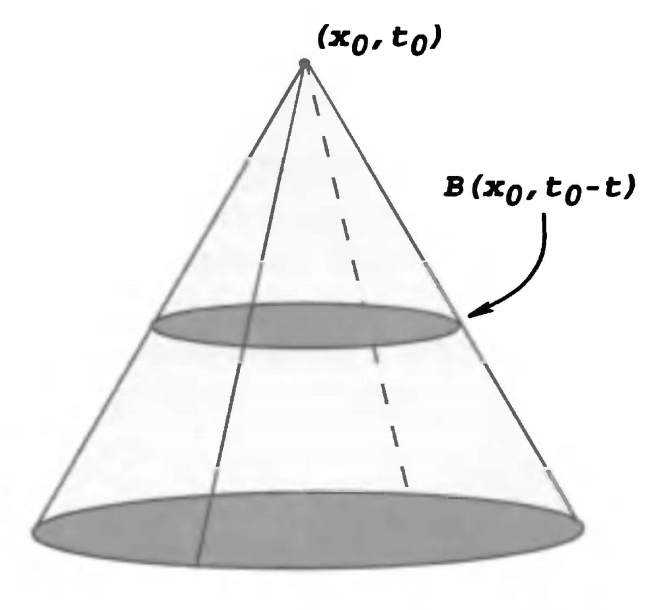
\includegraphics[scale=0.29]{Image/Cone of Dependence.png}
    \caption{Cone of Dependence}
\end{figure}
\begin{theorem}
If $u\equiv u_t\equiv 0$ on $B(x_0,t_0)\times\{t=0\}$, then $u\equiv 0$ within the cone $K(x_0,t_0)$.
\end{theorem}
In particular, we see that any "disturbance" originating outside $B(x_0, t_0)$ has no effect on the solution within $K(x_0, t_0)$ and consequently has finite propagation speed. We already know this from the representation formulas, at least assuming $g=u$ and$ h=U_t$ on $\mathbb{R}^n\times\{t=0\}$ are sufficiently smooth. The point is that energy methods provide a much simpler proof.
\begin{proof}
Define the local energy 
$$
e\left( t \right) =\frac{1}{2}\int_{B\left( x_0,t_0-t \right)}{u_{t}^{2}\left( x,t \right) +\left| Du\left( x,t \right) \right|^2\mathrm{d}x},\hspace{0.5cm}\left( 0\le t\le t_0 \right) 
$$
then 
$$
\begin{aligned}
\dot{e}\left( t \right) &=\int_{B\left( x_0,t_0-t \right)}{u_tu_{tt}+Du\cdot Du_t\mathrm{d}x}-\frac{1}{2}\int_{\partial B\left( x_0,t_0-t \right)}{u_{t}^{2}+\left| Du \right|^2\mathrm{d}S}
\\
&=\int_{B\left( x_0,t_0-t \right)}{u_t\left( u_{tt}-\Delta u \right) \mathrm{d}x}+\int_{\partial B\left( x_0,t_0-t \right)}{\frac{\partial u}{\partial \nu}u_t\mathrm{d}S}-\frac{1}{2}\int_{\partial B\left( x_0,t_0-t \right)}{u_{t}^{2}+\left| Du \right|^2\mathrm{d}S}
\\
&=\int_{\partial B\left( x_0,t_0-t \right)}{\frac{\partial u}{\partial \nu}u_t-\frac{1}{2}u_{t}^{2}-\frac{1}{2}\left| Du \right|^2\mathrm{d}S}.
\end{aligned}
$$
Now by Cauchy-Schwartz's inequality we have 
$$
\left| \frac{\partial u}{\partial \nu}u_t \right|\le \left| u_t \right|\cdot \left| Du \right|\le \frac{1}{2}u_{t}^{2}+\frac{1}{2}\left| Du \right|^2,
$$
which gives $\dot{e}(t)\le 0$ and hence $e(t)\le e(0)=0$ for all $0\le t\le t_0$. Thus $u_t,Du\equiv 0$ and consequently $u\equiv 0$ within the cone $K(x_0,t_0)$.
\end{proof}